\documentclass[graybox,envcountchap,sectrefs]{svmono_mod}
%\documentclass[envcountsame,envcountchap]{svmono}
% choose options for [] as required from the list in the Reference Guide

\usepackage{amsmath}
\usepackage{amsfonts}
\usepackage{amssymb}
\usepackage{mathptmx}
\usepackage{helvet}
\usepackage{courier}
%
\usepackage{type1cm}         
\usepackage{makeidx}         % allows index generation
\usepackage{graphicx}        % standard LaTeX graphics tool
                             % when including figure files
\graphicspath{{Figures/}}
\usepackage{multicol}        % used for the two-column index
\usepackage[bottom]{footmisc}% places footnotes at page bottom
\usepackage{array,booktabs,calc}

\usepackage{listings}
\usepackage[final]{pdfpages}
% see the list of further useful packages in the Reference Guide

\usepackage{enumerate}
\usepackage{tikz,pgfplots}
\usetikzlibrary{arrows.meta,quotes}
\usepackage[mode=buildnew]{standalone}

\usepackage{bbold}
\usepackage{bm}
\usepackage{hyperref}
\usepackage{capt-of}

% To insert a table of contents at the begining of each chapter
\usepackage{etoc}

% This is to neutralize the \textcolor command
% (command \usepackage[monochrome]{xcolor} does not work, likely because the cls file
%  modifies it)
\let\oldtextcolor\textcolor
\renewcommand{\textcolor}[2]{#2}
%\let\oldcolor\color
%\renewcommand{\color}[2]{#2}

% Some modifications
%1)The following piece of code has been taken from the Internet and redefines the \widebar command to make it look better (and better than overline)
\makeatletter
\let\save@mathaccent\mathaccent
\newcommand*\if@single[3]{%
  \setbox0\hbox{${\mathaccent"0362{#1}}^H$}%
  \setbox2\hbox{${\mathaccent"0362{\kern0pt#1}}^H$}%
  \ifdim\ht0=\ht2 #3\else #2\fi
  }
%The bar will be moved to the right by a half of \macc@kerna, which is computed by amsmath:
\newcommand*\rel@kern[1]{\kern#1\dimexpr\macc@kerna}
%If there's a superscript following the bar, then no negative kern may follow the bar;
%an additional {} makes sure that the superscript is high enough in this case:
\newcommand*\widebar[1]{\@ifnextchar^{{\wide@bar{#1}{0}}}{\wide@bar{#1}{1}}}
%Use a separate algorithm for single symbols:
\newcommand*\wide@bar[2]{\if@single{#1}{\wide@bar@{#1}{#2}{1}}{\wide@bar@{#1}{#2}{2}}}
\newcommand*\wide@bar@[3]{%
  \begingroup
  \def\mathaccent##1##2{%
%Enable nesting of accents:
    \let\mathaccent\save@mathaccent
%If there's more than a single symbol, use the first character instead (see below):
    \if#32 \let\macc@nucleus\first@char \fi
%Determine the italic correction:
    \setbox\z@\hbox{$\macc@style{\macc@nucleus}_{}$}%
    \setbox\tw@\hbox{$\macc@style{\macc@nucleus}{}_{}$}%
    \dimen@\wd\tw@
    \advance\dimen@-\wd\z@
%Now \dimen@ is the italic correction of the symbol.
    \divide\dimen@ 3
    \@tempdima\wd\tw@
    \advance\@tempdima-\scriptspace
%Now \@tempdima is the width of the symbol.
    \divide\@tempdima 10
    \advance\dimen@-\@tempdima
%Now \dimen@ = (italic correction / 3) - (Breite / 10)
    \ifdim\dimen@>\z@ \dimen@0pt\fi
%The bar will be shortened in the case \dimen@<0 !
    \rel@kern{0.6}\kern-\dimen@
    \if#31
      \overline{\rel@kern{-0.6}\kern\dimen@\macc@nucleus\rel@kern{0.4}\kern\dimen@}%
      \advance\dimen@0.4\dimexpr\macc@kerna
%Place the combined final kern (-\dimen@) if it is >0 or if a superscript follows:
      \let\final@kern#2%
      \ifdim\dimen@<\z@ \let\final@kern1\fi
      \if\final@kern1 \kern-\dimen@\fi
    \else
      \overline{\rel@kern{-0.6}\kern\dimen@#1}%
    \fi
  }%
  \macc@depth\@ne
  \let\math@bgroup\@empty \let\math@egroup\macc@set@skewchar
  \mathsurround\z@ \frozen@everymath{\mathgroup\macc@group\relax}%
  \macc@set@skewchar\relax
  \let\mathaccentV\macc@nested@a
%The following initialises \macc@kerna and calls \mathaccent:
  \if#31
    \macc@nested@a\relax111{#1}%
  \else
%If the argument consists of more than one symbol, and if the first token is
%a letter, use that letter for the computations:
    \def\gobble@till@marker##1\endmarker{}%
    \futurelet\first@char\gobble@till@marker#1\endmarker
    \ifcat\noexpand\first@char A\else
      \def\first@char{}%
    \fi
    \macc@nested@a\relax111{\first@char}%
  \fi
  \endgroup
}
\makeatother









% Macros for easier typing
%%%%%%%%%%%%%%%%%%%%%%%%%%%%
%%% Definiciones de comandos

%%% Operadores de decision
\def\dunodcero{\,\, \underset{D=0}{\overset{D=1}{\gtrless}}\,\,}
\def\dceroduno{\,\, \underset{D=1}{\overset{D=0}{\gtrless}}\,\,}
%\def\dunodcero{\begin{array}{c} D=1 \\ \gtrless \\ D=0 \end{array}}
%\def\dceroduno{\begin{array}{c} D=0 \\ \gtrless \\ D=1 \end{array}}

%%% Abreviaturas para PFA, PM  y PD.
\newcommand{\pfa}{P_{\text{FA}}} 
\newcommand{\pmis}{P_{\text{M}}} 
\newcommand{\pdet}{P_{\text{D}}} 
\newcommand{\appropto}{\mathrel{\vcenter{\offinterlineskip\halign{\hfil$##$\cr \propto\cr\noalign{\kern2pt}\sim\cr\noalign{\kern-2pt}}}}}

%%% Abreviaturas para Estimación
\newcommand{\EE}{\mathbb{E}}
\DeclareMathOperator*{\argmin}{argmin} % no space, limits underneath in displays
\DeclareMathOperator*{\argmax}{argmax} % no space, limits underneath in displays
\newcommand{\sML}{\hat{s}_\text{ML}}
\newcommand{\SML}{\hat{S}_\text{ML}}
\newcommand{\sMAP}{\hat{s}_\text{MAP}}
\newcommand{\SMAP}{\hat{S}_\text{MAP}}
\newcommand{\sMSE}{\hat{s}_\text{MSE}}
\newcommand{\SMSE}{\hat{S}_\text{MSE}}
\newcommand{\sMAD}{\hat{s}_\text{MAD}}
\newcommand{\SMAD}{\hat{S}_\text{MAD}}
\newcommand{\ejw}{e^{j\omega}}

%%% Abreviaturas para filtrado
\newcommand{\X}{{\mathbf X}}
\newcommand{\x}{{\mathbf x}}
\newcommand{\s}{{\mathbf s}}
\newcommand{\uu}{{\mathbf u}}
\newcommand{\UU}{{\mathbf U}}
\newcommand{\PP}{{\mathbf P}}
\newcommand{\Ruu}{{\mathbf R}_{uu}}
\newcommand{\rux}{{\mathbf r}_{ux}}
\newcommand{\hRuu}{\hat{\mathbf R}_{uu}}
\newcommand{\hrux}{\hat {\mathbf r}_{ux}}
\newcommand{\pp}{{\mathbf r}}
\newcommand{\eye}{{\mathbf I}}
\newcommand{\Normal}{{\mathcal N}}
\newcommand{\bigO	}{{\mathcal O}}

%%% Otras
\newcommand{\px}{p_X(x)}
\newcommand{\py}{p_Y(y)}

%%% Para procesos estocasticos
\newcommand{\jw}{j \omega}
 


%%%%%%%%%%%%%%%%%%%%%%%%%%%%%%%%%%%%%%%%%%%%%%%%%%%%%%%%%%%%%%%%%%%%%
\begin{document}

\author{Jer\'onimo Arenas-Garc\'ia, Jes\'us Cid-Sueiro, Vanessa G\'omez-Verdejo}
\title{Estimation Theory}
\subtitle{Year 2021-22}
% \maketitle

\frontmatter

\mainmatter %%%%%%%%%%%%%%%%%%%%%%%%%%%%%%%%%%%%%%%%%%%%%%%%%%%%%%%

%%%%%%%%%%%%%%%%%%%%%%%%%%%%%%%%%%%%%%%
\chapter{Statistical Estimation Theory}
%\section{Introduction to the Estimation Problem}
\label{sec:M2}

The contents of this lesson cover an introduction to the estimation problems. So, during this session, we will present some basic concepts of estimation design using statistical information. Important concepts, such as {\em a priori} and {\em a posteriori} probabilities, observations, cost functions, or likelihoods will be illustrated through a series of simple examples.

\subsection{Example 1: Bayesian estimation without observations}
\label{subsec:example1}

\begin{problem} 
A food delivery company wants to develop a new service to estimate the time that will elapse from the reception of an order to its delivery to the customer's home.
To do this, the total service or delivery time, $S$, is modelled as a random variable given by the sum of two independent r.v.s:
$$S=T_1 + T_2,$$
where $T_1$ models the time (in minutes) needed to prepare the order and $T_2$ is the shipping time (in minutes).
Analyzing these times the company has characterized r.v.s $T_1$ and $T_2$ with the following probability distributions:

$$p_{T_1}(t_1) = 0.5 \exp{\left[-0.5(t_1 - 10) \right]} \quad \quad  t_1 >10 $$
$$p_{T_2}(t_2) = \frac{0.2}{r} \exp{\left[-\frac{0.2}{r} (t_2-5)\right]} \quad \quad  t_2 >5 $$
where r is the distance (in kilometers) from the company store to the customer's home. 
To estimate the value of $S$, let's start solving the following questions:
    \begin{itemize}
        \item[a)] Knowing the probability distributions of $T_1$ and $T_2$, can we obtain the probability distribution of $S$?
        \item[b)] Knowing the probability distribution of $S$, can we estimate the total delivery time? 
        \item[c)] Which is the optimal estimator for a given cost? 
    \end{itemize}
\end{problem}

\begin{solution} 

\begin{itemize}
\item[a)] Can we obtain the probability distribution of $S$? \\
Computing the distribution of $S$ requires applying a change of random variable in which we have to transform two random variables ($T_1$ and $T_2$) into a new variable ($S$). Since $S$ is the sum of two independent random variables, we know that their distribution will be given by the convolution of the distributions of $T_1$ and $T_2$: 
$$ p_S(s) = p_{T_1} (t_1=s) \ast  p_{T_2} (t_2=s)  = \int  p_{T_1} (t_1=s)  p_{T_2} (t_2=s-t_1) d t_1   $$
after some mathematical manipulations (the complete mathematical development is left as an exercise), we can see that $p_S(s)$ is given by the following expression (see Figure \ref{Fig_ps}):
$$ p_S(s) = \left(0.5 + \frac{0.2}{r}\right) \left(s -15\right) \exp{\left[-\left(0.5 + \frac{0.2}{r}\right) \left(s-15\right)  \right]}   \quad  s >15$$

\begin{figure}[!t]
\begin{center}
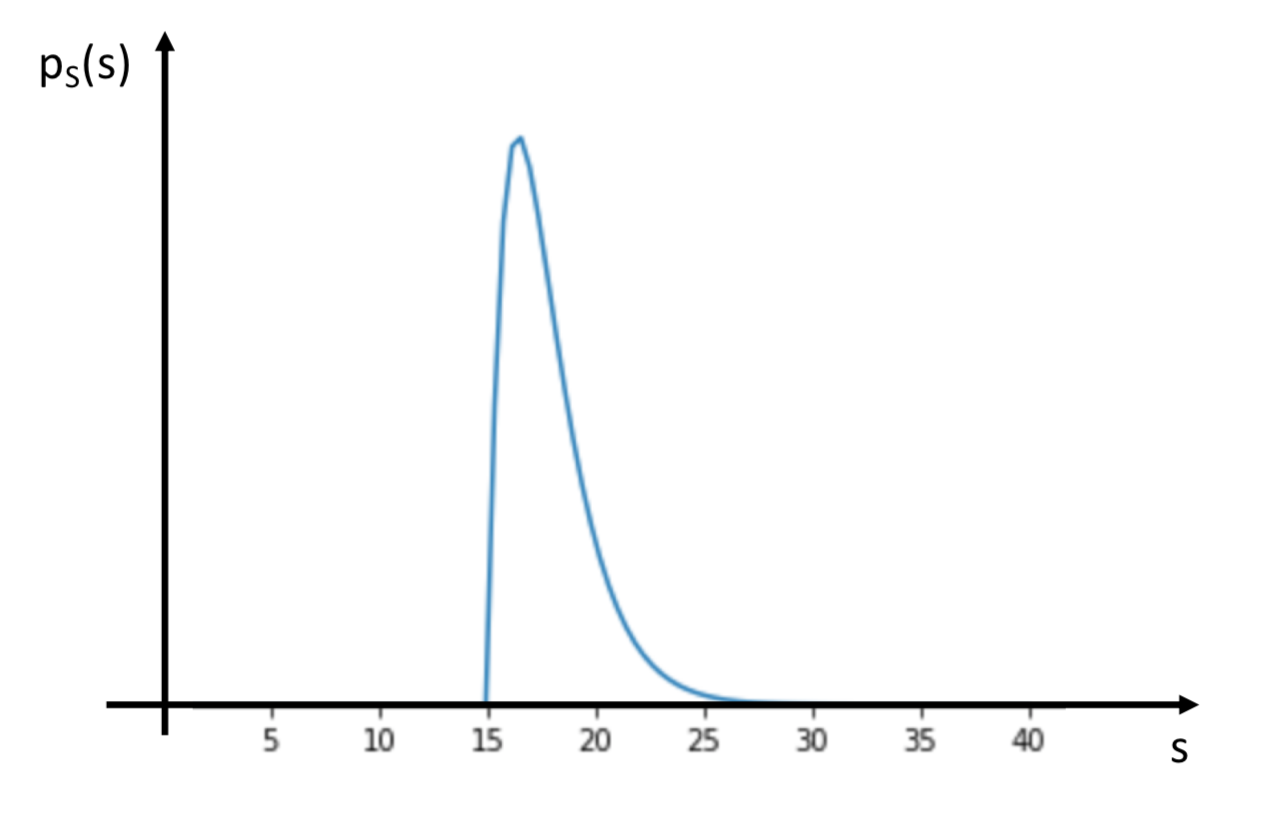
\includegraphics[scale=.25]{Figures/Fig_MC1_1.png}
\caption{Representation of the probability distribution of $S$ for $r=1$.}
\label{Fig_ps}
\end{center}
\end{figure}
\vspace{0.2cm}
\item[b)] Can we now estimate the total delivery time?\\
Let's consider that we receive an order to be delivered to one kilometer of distance ($r=1$Km), so we have that 
$$ p_S(s) = 0.7 \left(s -15\right) \exp{\left[-0.7 \left(s-15\right)  \right]}   \quad  s >15.$$
Knowing this distribution, we can know which values of $S$ are most probable and which values are completely unlikely; for instance, analyzing Figure \ref{Fig_ps}, we can realize that it is quite likely that $S$ is between $15$ and $20$, whereas it is impossible that it is lower than $15$, and it is almost impossible that it is greater than $30$. So,  in light of the distribution of $S$, we can estimate the total delivery time considering different criteria (see Figure \ref{Fig_ps_s1_s2}):

\begin{figure}[!t]
\begin{centering}
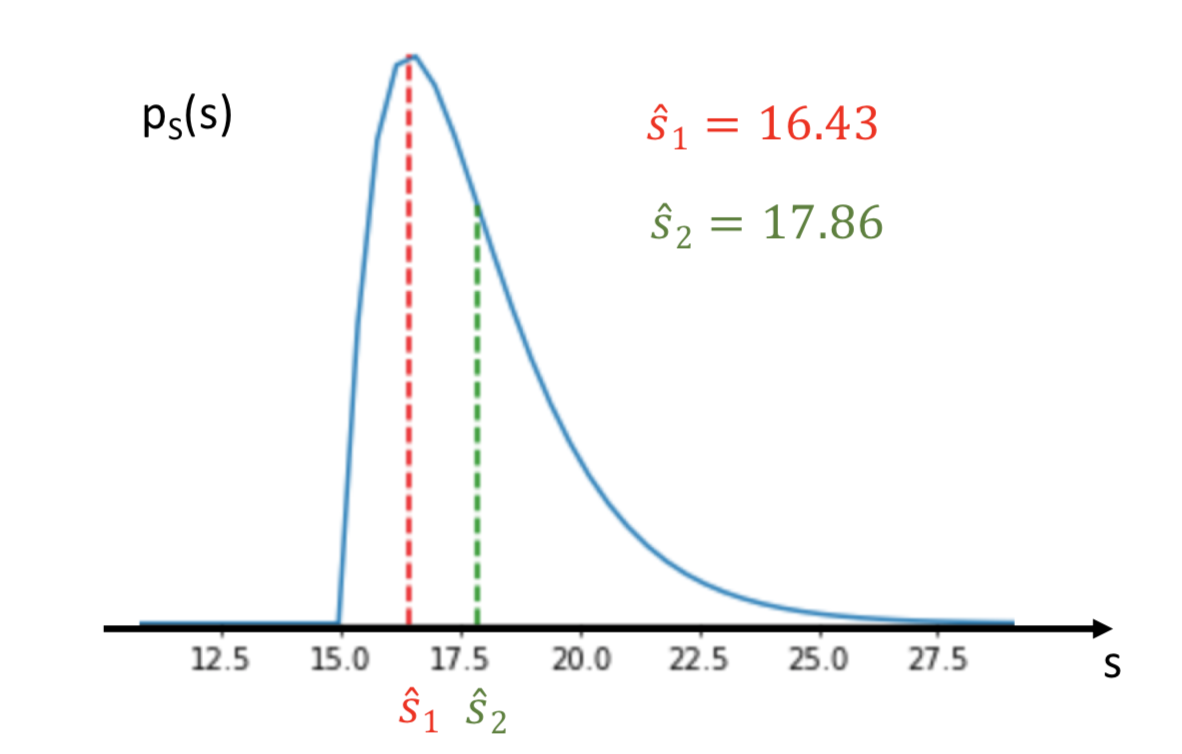
\includegraphics[scale=.25]{Figures/Fig_MC1_2.png}
\caption{Some possibles estimators of $S$ analyzing $p_S(s)$.}
\label{Fig_ps_s1_s2}
\end{centering}
\end{figure}

\begin{itemize}
\item One could consider that a good estimation could be given by the most likely value of $S$, that is, by the mode of $S$:
$$ \hat{s}_1  = {\arg\max_s}  p_S(s) $$
and we can compute this value by deriving $p_S(s)$ and setting the result to zero:

$$  \left.\frac{\partial p_S(s)}{\partial s} \right|_{s = \hat{s}_1} = 0.7 \exp{\left[-0.7 \left(\hat{s}_1 -15\right) \right]} - 0.7^2 \left(\hat{s}_1 -15\right) \exp{\left[-0.7 \left(\hat{s}_1 -15\right)  \right]} =0$$
Now, we can cancel the term\footnote{Note that by cancelling this term we are skipping the solution $\hat{s}_1 \rightarrow \infty$, but analyzing the shape of $p_S(s)$ we can check that this root is a minimum.} $0.7\exp{\left[-0.7 \left(\hat{s}_1 -15\right) \right]}$ and get:

$$ 1 - 0.7( \hat{s}_1 -15) =0$$
$$ \hat{s}_1  = 15 + \displaystyle \frac{1}{0.7}= 16.43~ {\rm min.}$$
To complete this calculation, we have to check that this solution is a maximum (the derivative only guarantees returning relative extremes or saddle points). We can do this either analyzing the shape of $p_S(s)$ or checking that the second derivative is negative.
\item Another possible estimation could be given by the expected value of $S$,
$$  \hat{s}_2 = \mathbb{E}\{S\} = \int s p_S(s) ds =  \int_{15}^{\infty} 0.7 s \left(s -15\right) \exp{\left[-0.7 \left(s-15\right)  \right]} ds $$
and solving this integral by parts, we have
$$ \hat{s}_2 =   15 + \displaystyle \frac{2}{0.7}=17.86~{\rm min.}$$
\item Or we could even raise other estimators, such as the median of the distribution or the 25\% or 75\% percentiles. 
\end{itemize}

Finally, it is important to bear in mind that regardless of the estimator we use, we probably have an estimation error (it is practically impossible for the estimated value to coincide with the actual one) and the error of each estimator will indicate us which estimator is more adequate. %In fact, if we know how our problem is going to measure the different errors (what the cost function gives us), the ideal is for us to design the estimator trying to minimize this cost. 
In fact, in this unit we will pursue as a design criterion the minimization of the mean value of a cost criterion that establishes how we should penalize different kinds of errors.

\vspace{0.2cm}
\item[c)] How can we find the optimal estimator for a given cost? 
For the design of the estimator, the food delivery company wants to minimize the following cost function (see Figure \ref{Fig_MC1_5}):
\begin{equation} 
c(\hat{s},s) = \begin{cases}
0.005|s-\hat{s}| & {\rm if} \quad \hat{s}>s\\
0.1|s-\hat{s}|  & {\rm if} \quad \hat{s}<s 
\end{cases} \nonumber
\end{equation} 

%{\color{red} Podemos dar un significado a este coste? Perdidas en Keuros? Pero en ese caso siempre pierde... y no tiene sentido definir costes negativos que serían beneficios.... Ponemos unas ganancias máximas y esto son perdidas sobre esas ganacias....???}

\begin{figure}[!t]
\begin{tabular}{m{.1\textwidth}m{.5\textwidth}m{.4\textwidth}}
&\raisebox{-18ex}{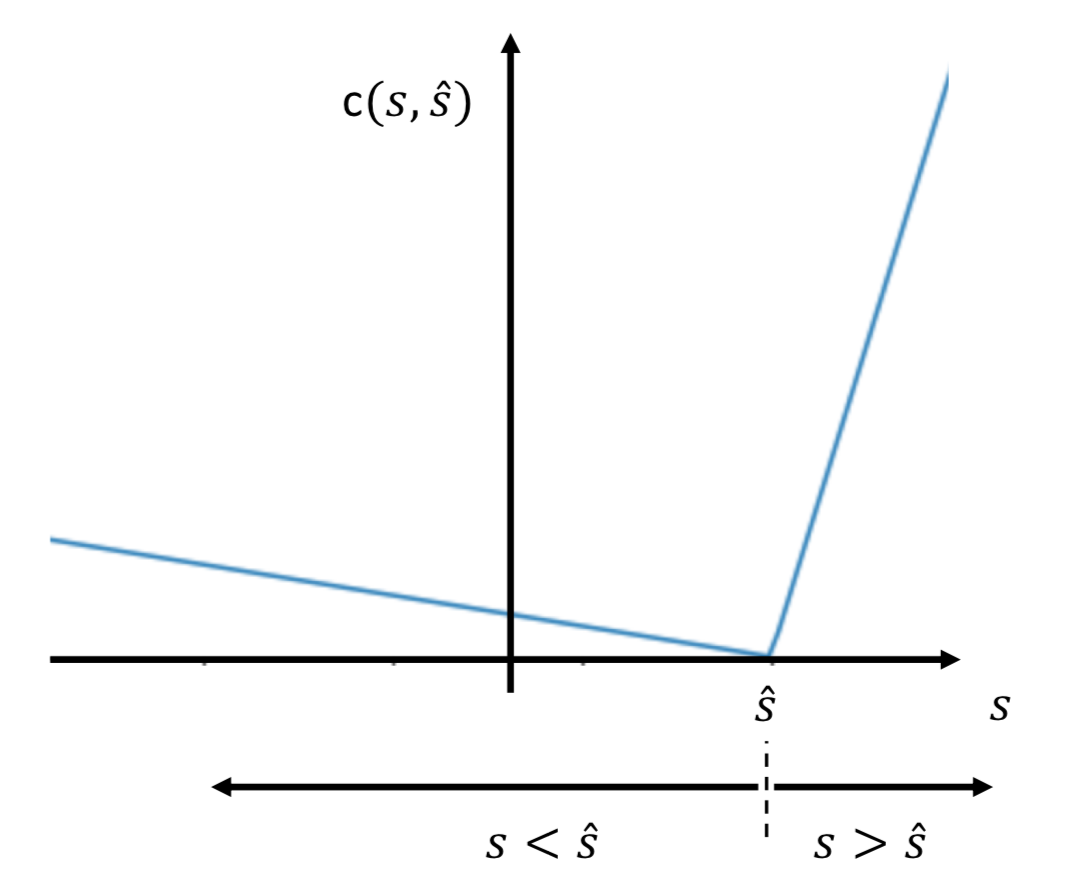
\includegraphics[scale=.25]{Figures/Fig_MC1_5.png}}&
 \begin{equation} 
c(\hat{s},s) = \begin{cases}
0.005|s-\hat{s}| & {\rm if} \quad \hat{s}>s\\
0.1|s-\hat{s}|  & {\rm if} \quad \hat{s}<s 
\end{cases} \nonumber
\end{equation} 
\end{tabular}
\caption{Asymmetric cost function to be minimized during the estimator design.}
\label{Fig_MC1_5}
\end{figure}

As any cost function, this cost function indicates how we have to penalize the fact that the estimated value differs from the actual value of $S$. However, unlike typical cost functions, this is an asymmetric cost function (see Figure \ref{Fig_MC1_5}), that is, it applies different penalties in case of overestimating the values of $S$ ($\hat{s} >s $) or underestimating them ($\hat{s} <s $). In this way, this cost function is indicating that if the order arrives before the time we have estimated it will penalize less than in case the customer has to be waiting longer than expected, i.e., if our  order takes longer to arrive than we have estimated. In this case, using the mean or median of $S$ is not the most appropriate estimator, and we should choose a value higher than the expected one. I.e., since subestimations of the actual time of delivery are highly penalized, we should try to be conservative and produce estimators that are only rarely exceeded. So, it is possible that a value around the 70\%-80\% percentile of the $p_S(s)$ distribution is close to the estimator we are looking for.


Reviewing the expression of the cost function to be minimized, we can see that the cost value depends both on the estimator $\hat{s}$ and on the random variable to be estimated $S$. So, as the cost function is a function of a random variable, it is itself another random variable. For this reason, we are going to denote it as $ C = c(\hat{s},S)$.

\begin{figure}[!t]

\begin{tabular}{m{.5\textwidth}m{.5\textwidth}}
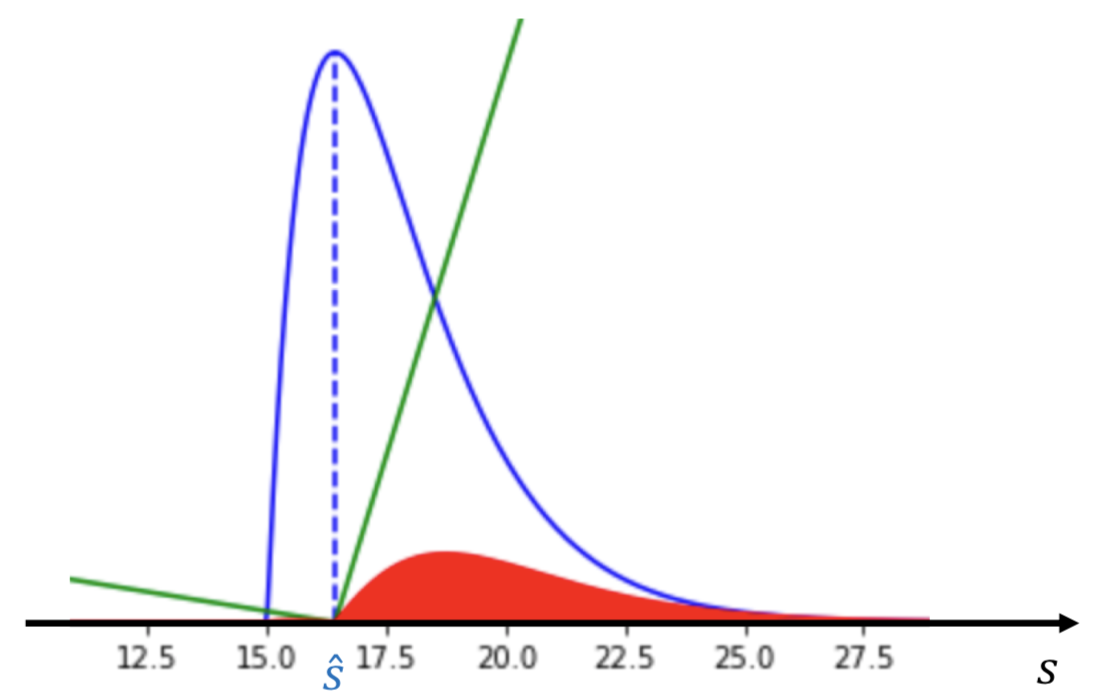
\includegraphics[scale=.3]{Figures/Fig_MC1_6.png}&
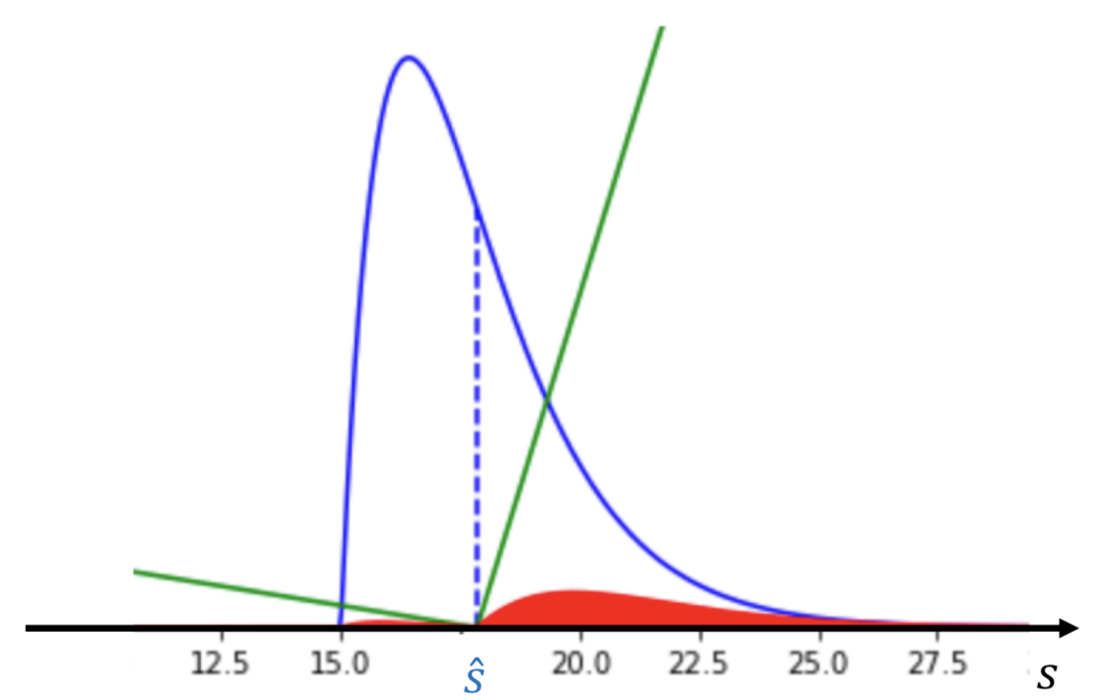
\includegraphics[scale=.3]{Figures/Fig_MC1_7.png}\\
(a) $\hat{s} = 16.43 \quad \mathbb{E}\{C\} = 0.23$ &
(b) $\hat{s} =  17.86 \quad  \mathbb{E}\{C\} = 0.12 $ \\
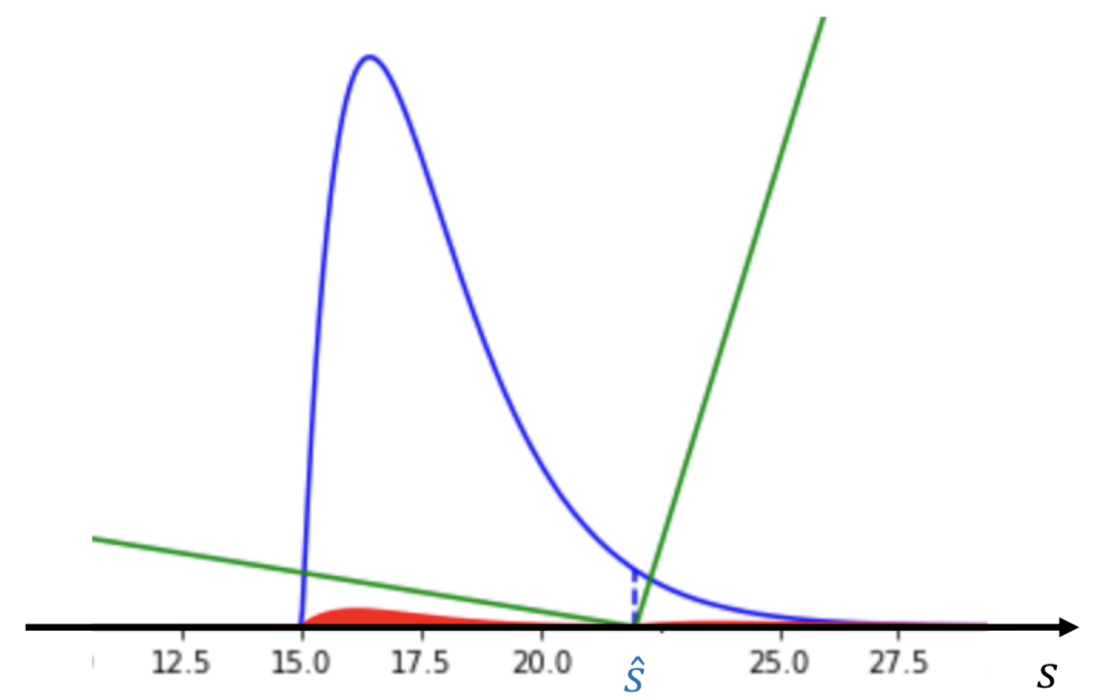
\includegraphics[scale=.3]{Figures/Fig_MC1_8.png}&
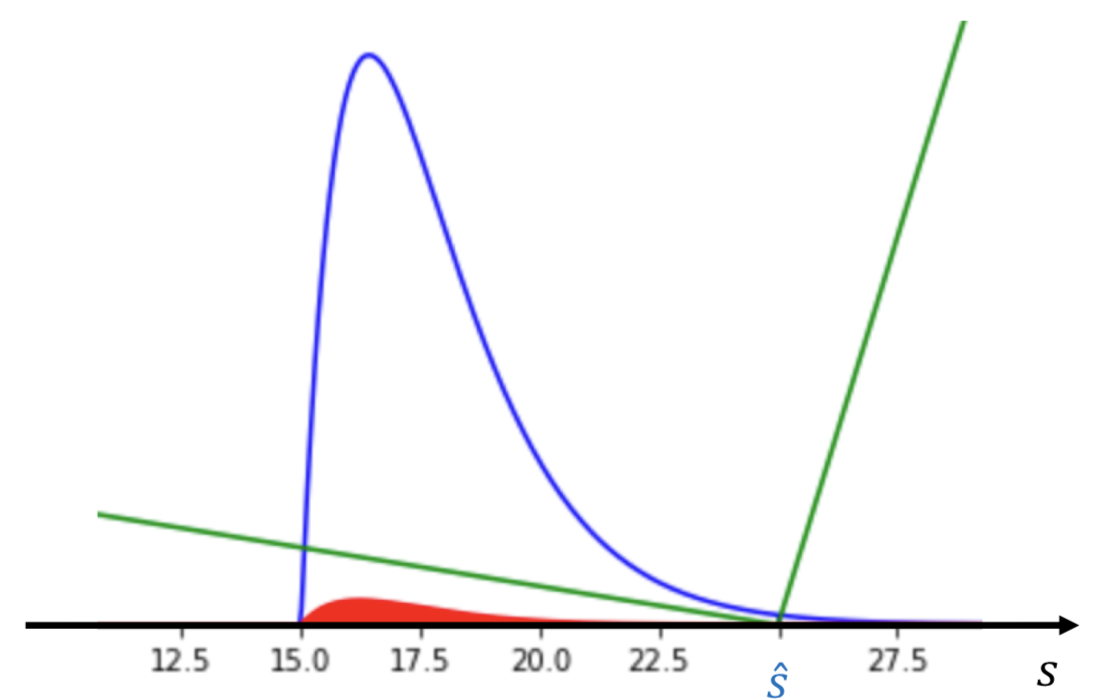
\includegraphics[scale=.3]{Figures/Fig_MC1_9.png}\\
(c) $\hat{s} = 22  \quad \mathbb{E}\{C\}= 0.04$ &
(d) $\hat{s} =  25 \quad \mathbb{E}\{C\}=0.05$ \\
\multicolumn{2}{c}{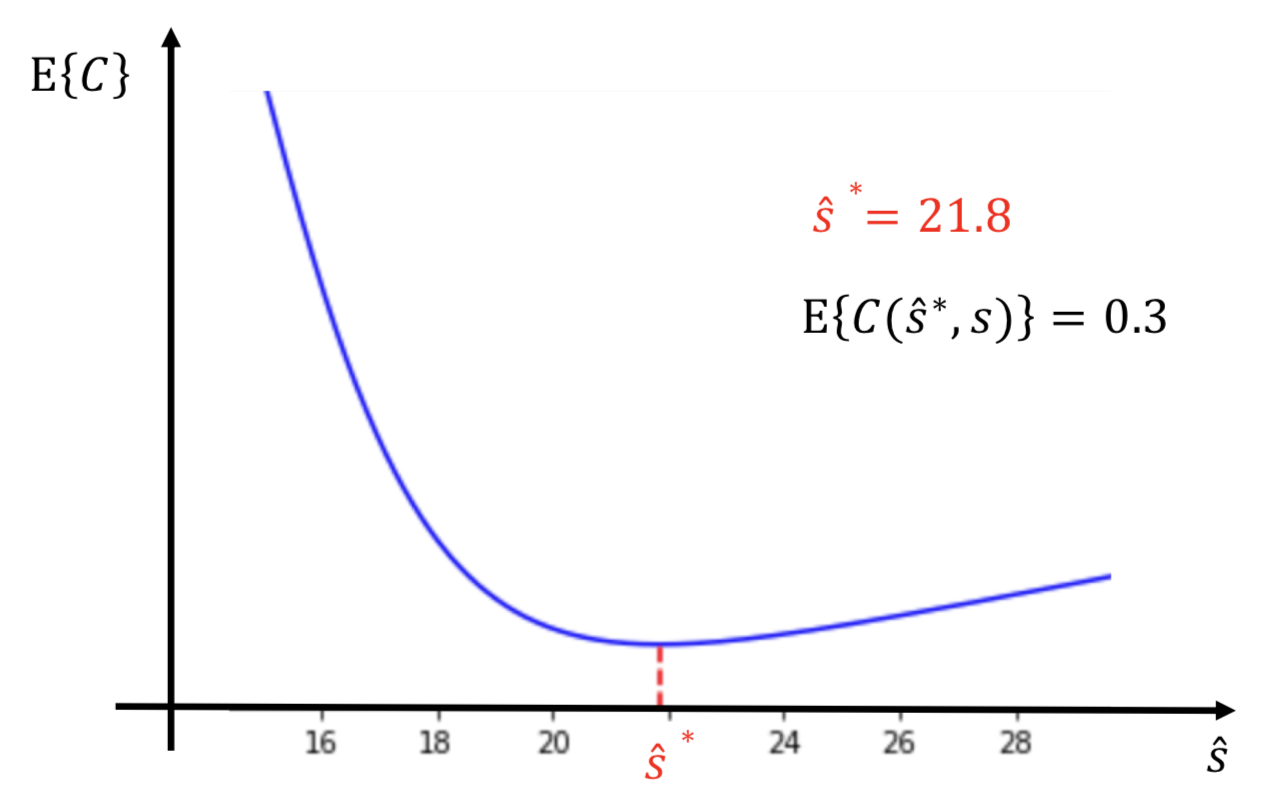
\includegraphics[scale=.25]{Figures/Fig_MC1_10.png}}\\
\multicolumn{2}{c}{(e) Evolution of the mean cost with the value of $\hat{s}$}
\end{tabular}
\caption{Process of minimization of the mean cost for different values of the estimator.}
\label{Fig_MC1_6_9}
\end{figure}

When we wanted to find the value of the estimator that minimizes the cost $C$, we would have to find the value of the estimator which minimizes the expected cost or the mean cost. So, the optimum estimator would be given by:
$$ \hat{s}^{*} = \arg\min_s~ \mathbb{E}\{C\} = \arg\min_{\hat{s}}~ \mathbb{E}\{c(\hat{s},S)\}$$
where the mean cost is computed as:
$$\mathbb{E}\{c(\hat{s},S)\} = \int c(\hat{s},s) p_s(s) ds$$


For each possible value of the estimator, we will get a different mean cost, and we will have to select the estimator value that provides the minimum mean cost. Fig \ref{Fig_MC1_6_9} shows the average cost for different values of the estimator for the given asymmetric cost function. In fact, Subfigures \ref{Fig_MC1_6_9}(a)-(d) show how the mean cost is computed for different values of the estimator; note that the mean cost is computed as the area resulting from multiplying the distribution $p_S(s)$ by the cost function $c(\hat{s},S)$, and, as different values of the estimator, $\hat{s}$,  will place the cost function in different positions, this process will result in different mean costs. If we directly compute the mean cost for any possible value of $\hat{s}$ we would obtain a curve similar to that shown in Subfigure \ref{Fig_MC1_6_9}(e) and $\hat{s}^{*}$ would be the value of $\hat{s}$ which minimizes it. In this case, we can see that the optimum  estimator would be $\hat{s}^{*} = 21.8$ min and it generates a mean cost of $0.3$.


\end{itemize}
\end{solution}

\subsection{Example 2: Bayesian estimation with observations}
\label{subsec:example2}

\begin{problem}
To obtain a more accurate estimation of the delivery time, the company has improved the food preparation process, so that it is able to know the exact time it will take to prepare the order $T_1=t_1$. 

When we want to estimate the value of $S$ without observations, the only distribution which provides information about the value of $S$ is $p_S(s)$; however, when we have additional information such as knowledge of the value of $t_1$ (observation), including this information in our estimation problem makes the estimation of $S$ easier (more accurate). Adding this knowledge (observation) to the estimation task implies using the posterior distribution of $S$, $p_{S|t_1}(s|t_1)$, instead of using $p_S(s)$.

To solve the estimation problem in this new scenario, let's try to answer the following questions:
 \begin{itemize}
\item[a)] Can we obtain the probability distribution of $S$ given the value $T_1=t_1$?
\item[b)] Can we estimate the total delivery time for a given value $T_1=t_1$? 
\item[c)] Given a cost function to be optimized, which is the optimal estimator for a given value $T_1=t_1$? 
    \end{itemize}
\end{problem}

\begin{solution}
\begin{itemize}
\item[a)] Can we obtain the probability distribution of $S$ given the value $T_1=t_1$?\\
The calculation of the posterior distribution of $S$ can be done by applying the following r.v change\footnote{Note that as we are calculating the distribution of $S$ given $T_1$, the value of $T_1$ is known ($T_1=t_1$).}:
$$S = t_1 + T_2$$
so, $p_{S|t_1}(s|t_1)$ can be obtained by shifting the distribution of $p_{T_2}(t_2)$ to the position of $t_1$, i.e.,
$$p_{S|t_1}(s|t_1)=p_{T_2}(t_2=s-t_1) =
\frac{0.2}{r} \exp{\left[-\frac{0.2}{r} (s-t_1-5)\right]} \quad \quad  s >t_1 +5$$
%\begin{figure}[!h]
%\begin{center}
%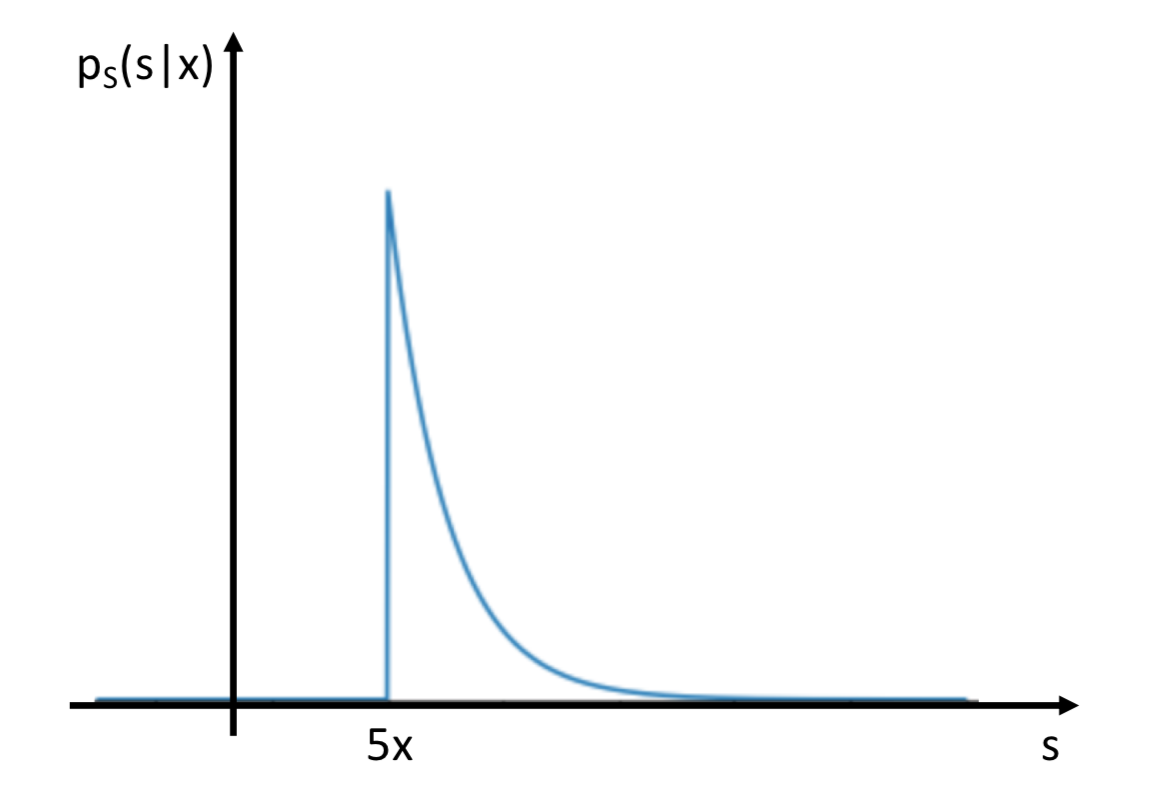
\includegraphics[scale=.25]{Figures/Fig_MC1_11.png}
%\end{center}
%\end{figure}


\item[b)] Can we estimate the total delivery time for a given value $T_1=t_1$? 

To answer this question, let's consider that a customer is calling the food company to place an order from a distance of one kilometer ($r=1$Km), and in this moment and for this order the preparation time is $t_1=12$ minutes. So we have:

$$p_{S|t_1}(s|t_1)=p_{T_2}(t_2=s-t_1) =
0.2 \exp{\left[-0.2 (s-17)\right]} \quad \quad  s >17$$

and, examining this distribution (see Figure \ref{p_S_x2}), we can consider different estimators such as the maximum of the distribution, which is $\hat{s}_1=17$ min., or the expected value of $S$ given $t_1=12$, which can be computed (by solving the integral by parts) as:

$$ \hat{s}_2= \mathbb{E}\{S|t_1=12\} = \int s p_{S|t_1}(s|t_1) ds = 17+\frac{1}{0.2} = 22 {\rm min.}$$

\begin{figure}[!t]
\begin{center}
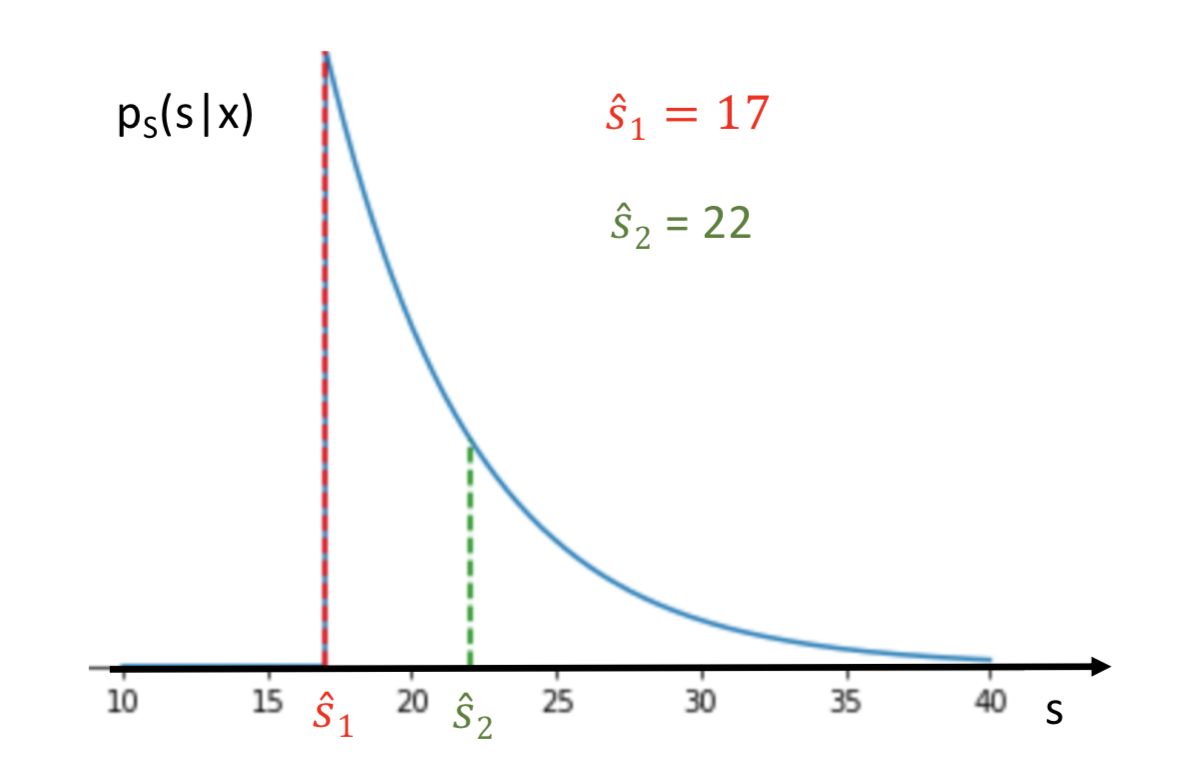
\includegraphics[scale=.25]{Figures/Fig_MC1_12.png}
\caption{Some possible estimators of $S$ given that $t_1=12$.}
\end{center}
\label{p_S_x2}
\end{figure}

For any value of the observation, the posterior distribution of $S$ will change (in this case, the $ p_{S|t_1}(s|t_1)$ will be shifted) and the value of the estimator will depend on the observation value ($t_1$). If we want to obtain a general expression for these estimators (for any value of $t_1$), we can directly compute both the maximum and the mean by using the expression of the posterior for any value of $t_1$ (we are still considering $r=1$):
$$ p_{S|t_1}(s|t_1) = 0.2 \exp{\left[-0.2 (s-t_1-5)\right]} \quad \quad  s >t_1 +5$$

For example:

\begin{itemize}
\item If we consider that the mode of $ p_{S|t_1}(s|t_1)$ could be an adequate estimator, the estimator will be:
$$ \hat{s}_1  = {\arg\max_s}  p_{S|t_1}(s|t_1) $$
In this case, as $p_{S|t_1}(s|t_1) $ is a decreasing function for $s >t_1 +5$, its maximum is 
$$\hat{s}_1 = t_1 +5.$$

\item We can also consider that the expected value of $S$ given $t_1$ is a good estimator. In this case (computing the integral by parts):
$$\hat{s}_2= \mathbb{E}\{S|t_1\} = \int s p_{S|t_1}(s|t_1) ds = 5 + t_1 +\frac{1}{0.2} = 10+t_1$$
\end{itemize}


However, in order to decide which estimator is best, we need, as before, to define which cost function we want to minimize.

\item[c)] Given a cost function to be optimized, which is the optimal estimator for a given value $T_1=t_1$? 

Again, when we are designing an estimator we may want to design it in such a way that it minimizes the mean value of a given cost function. Now, as we are now working with observations, our goal will be finding the optimal estimator for any observed value (for any given value of $T_1=t_1$). 

Thus, we can now find the optimum estimator by 
$$ \hat{s}^{*} = \arg\min_s~ \mathbb{E}\{c(\hat{s},S)|t_1\}$$
where 
$$\mathbb{E}\{c(\hat{s},S)|t_1\} = \int c(\hat{s},s) p_{S|t_1}(s|t_1)  ds$$


\begin{figure}[!t]
\begin{tabular}{m{.5\textwidth}m{.5\textwidth}}
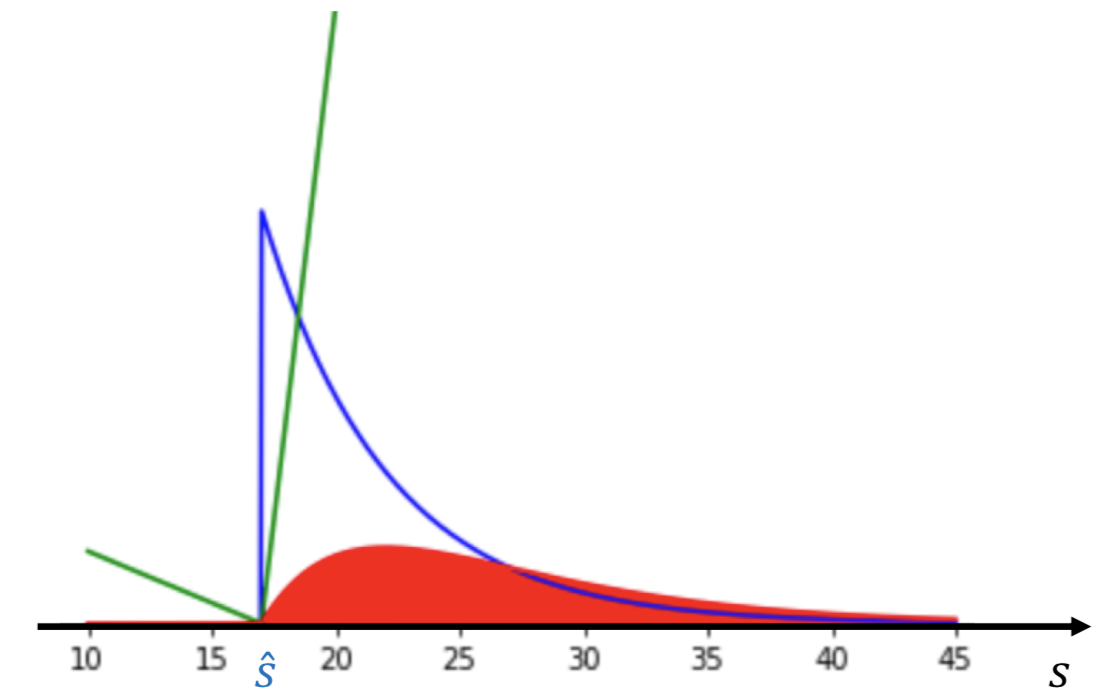
\includegraphics[scale=.3]{Figures/Fig_MC1_13.png}&
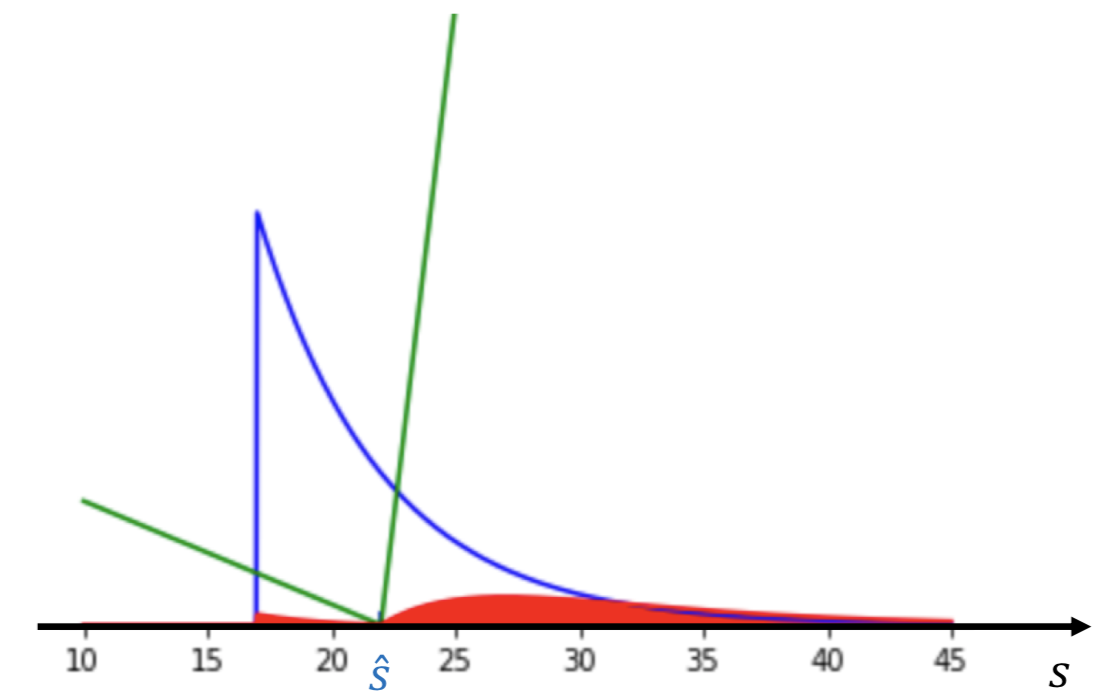
\includegraphics[scale=.3]{Figures/Fig_MC1_14.png}\\
(a) $\hat{s} = 17$ min. and  $ \mathbb{E}\{c(\hat{s},S)|x\} = 0.999$  &
(b) $\hat{s} = 12$ min. and $ \mathbb{E}\{c(\hat{s},S)|x\} = 0.385 $ \\
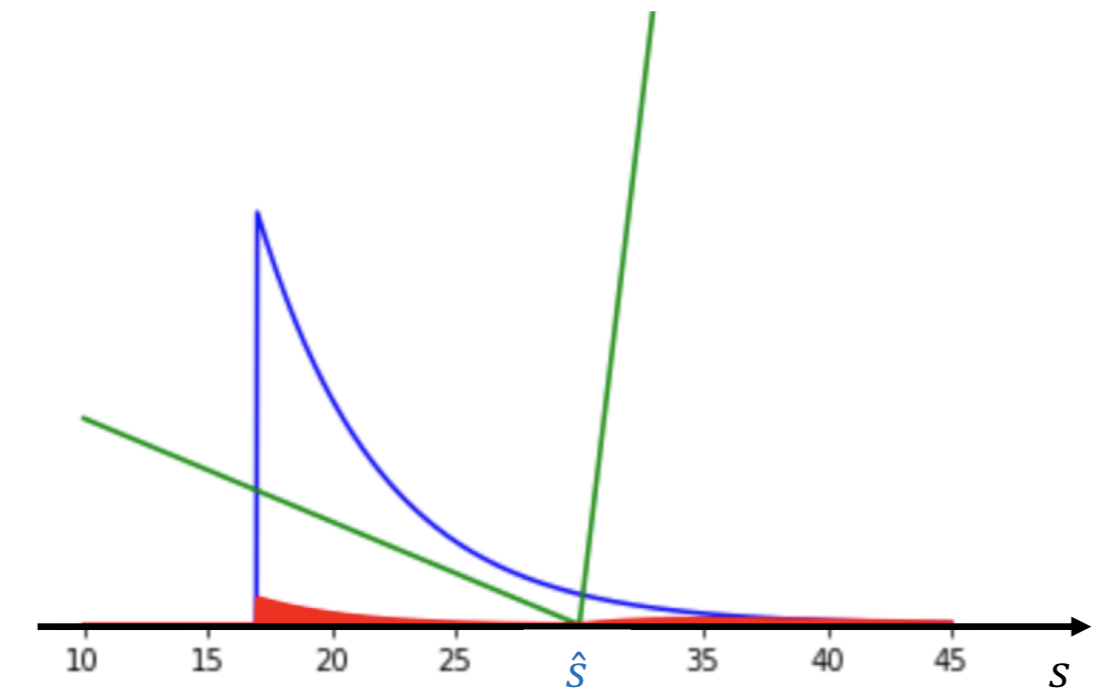
\includegraphics[scale=.3]{Figures/Fig_MC1_15.png}&
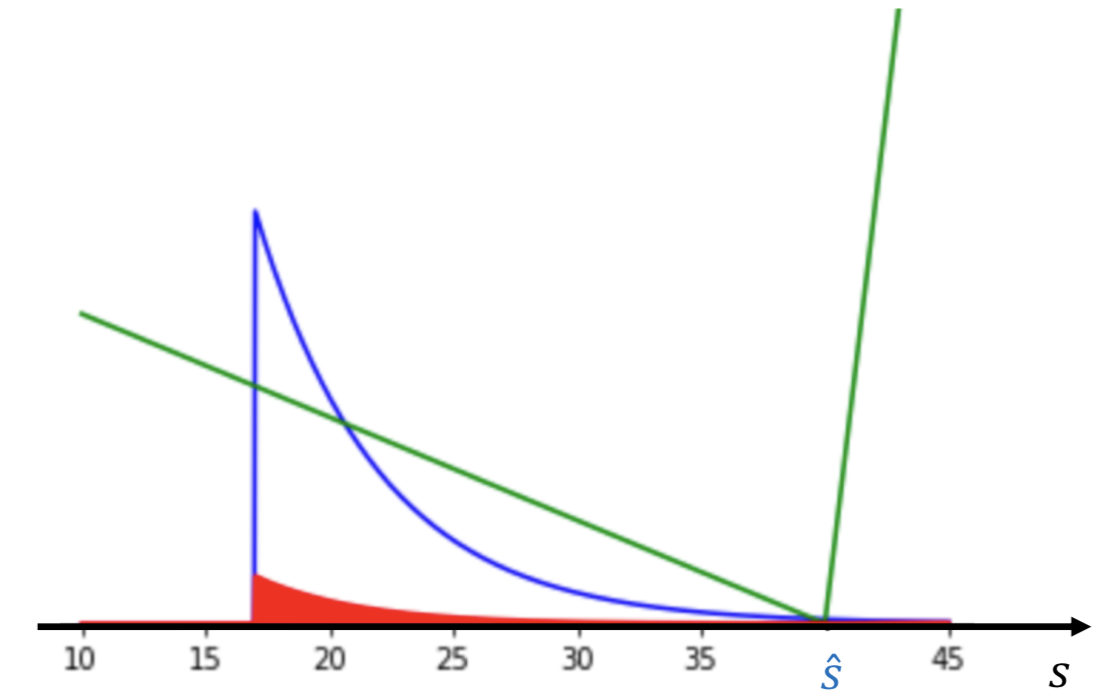
\includegraphics[scale=.3]{Figures/Fig_MC1_16.png}\\
(c) $\hat{s} = 30$ min. and  $\mathbb{E}\{c(\hat{s},S)|x\}= 0.158$ &
(d) $\hat{s} = 40$ min. and  $\mathbb{E}\{c(\hat{s},S)|x\}=0.169$ \\
\multicolumn{2}{c}{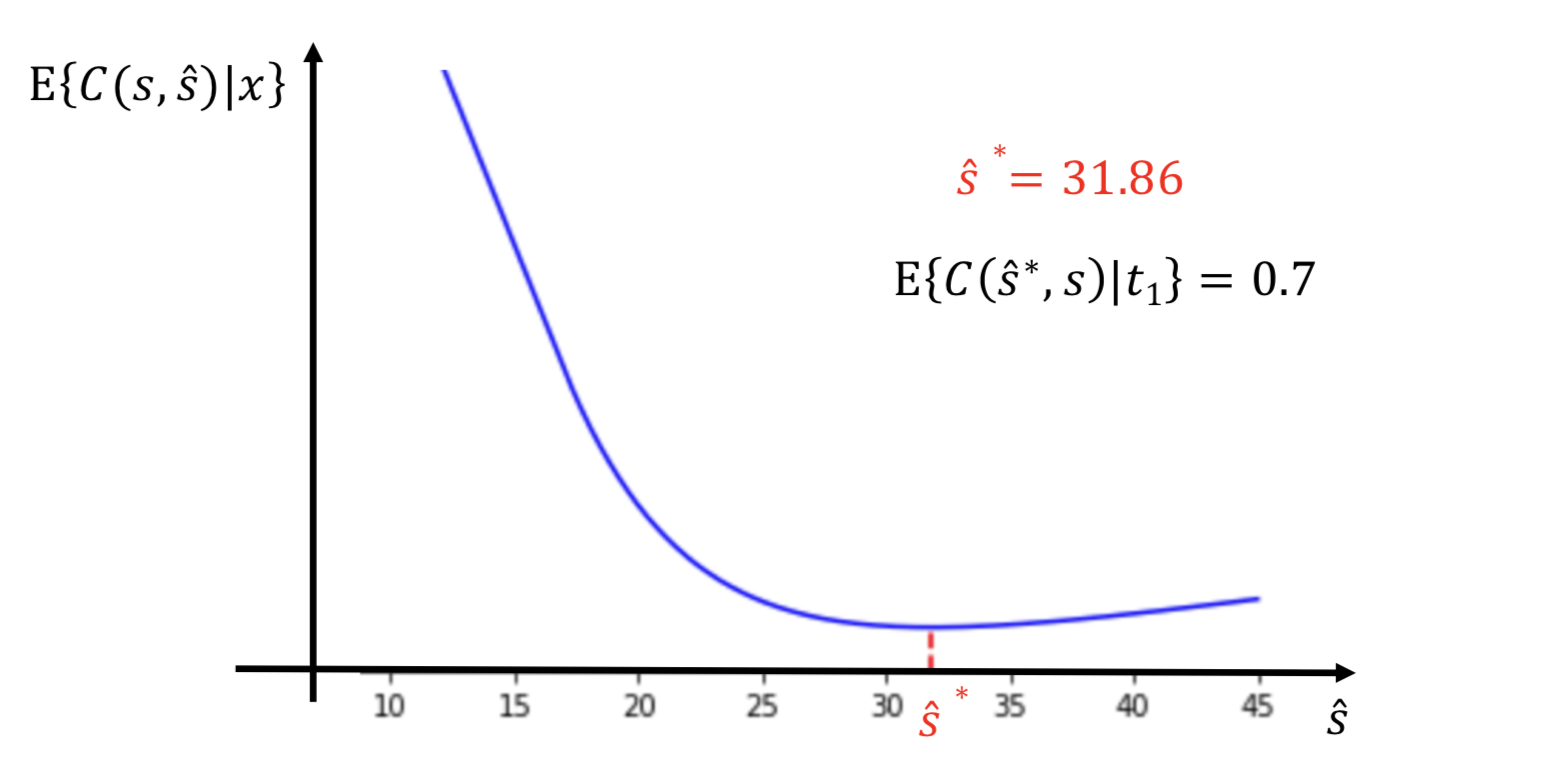
\includegraphics[scale=.25]{Figures/Fig_MC1_17.png}}\\
\multicolumn{2}{c}{(e) Evolution of the mean cost given  $t_1$ with the value of $\hat{s}$}
\end{tabular}
\caption{Process of minimization of the mean cost given $t_1$ for different values of the estimator.}
\label{Fig_MC1_13_17}
\end{figure}

Once again, each possible value of the estimator will provide a different mean cost for a given value of $t_1$ and our goal will be to select the estimator that minimizes said mean cost. 
Summarizing our example problem:
\begin{itemize}
\item An order is placed to be shipped to a distance of one kilometer ($r=1$Km);
\item For this order the preparation time is $t_1=12$ minutes;
\item We want to minimize the asymmetric cost function used in Problem \ref{subsec:example1}(c);
\end{itemize}
Fig \ref{Fig_MC1_13_17} shows the procedure of minimizing the mean cost given $t_1=12$. Subfigures \ref{Fig_MC1_13_17}(a)-(d) plot the conditional mean costs for different values of the estimator and Subfigure \ref{Fig_MC1_13_17}(e) illustrates the mean cost as a function of $\hat{s}$. Analyzing these figures, we can check that the optimum estimator value is $\hat{s}^{*} = 31.86$ min and it generates a mean cost (given that $t_1 = 12$) of $0.7$.

%{\color{red} Creo que dejar lo siguiente estarí bien si pudieramos calcular la expresión analítica de $\hat{s}^{*}$ para cualquier $t_1$ y luego el coste medio global... Como analíticamente no es sencillo, no sé si es bueno dejarlo o no.... Otra cosa es hacerlo en python y poner la gráfica o algo asi.... En cualquier caso creo que habría que incluir indicando que el estimador es una función de las observaciones y su diseño consiste en encontrar esta función...}
Finally, it is important to note that the involved mean cost is for a value of $t_1=12$. If we wanted to compare this cost with that incurred by the estimator designed without observations, we would have to compute the optimum estimator and its mean cost (given the observation) for any value of $t_1$ and average these costs taking into account the probability of each $t_1$ value. %That is, we would have to compute the global mean cost of 

%Applying this procedure, we are computing an estimator for each value of $X=x$ and minimizing the mean cost given the observation, but are we minimizing the total cost?. The answer to this question is ``yes'', since from this relationship:
%\begin{eqnarray}
%\mathbb{E}\{c(\hat{S},S)\}  & =&  \int \int c(\hat{s},s) p_{S,X}(s,x)  ds dx \nonumber \\
%&=& \int \left[ \int c(\hat{s},s) p_{S|x}(s|x)  ds \right]  p(x) dx \nonumber  \\
%&=& \int \left[ \mathbb{E}\{c(\hat{s},S)|x\}  \right]  p(x) dx \nonumber  
%\end{eqnarray}
%allows us to claim that minimizing the mean cost given the observation for any value of $x$, we are minimizing the overall mean cost.
\end{itemize}
    
\end{solution}

%\subsection{Example 3: Maximum likelihood estimation}

%\begin{problem}
%Communication channel with gaussian noise
%$$X = S +N$$


%$$p_N(n) = G(0, v_N)$$

%We transmit signal $S$ and in the receptor we observe $X$, our goal is to estimate the transmitted value ($S$) with the observation of the signal in the receptor ($X$).
%\begin{itemize}
%\item[a)] Without additional information, can we estimate the value of $S$?
%\item[b)] Could we design a bayesian estimator (the optimum estimator for a given cost)?
%\end{itemize}
%\end{problem}

%\begin{solution}
%\begin{itemize}
%\item[a)] Without additional information, can we estimate the value of $S$?
%With the given information, the only distribution that we can easily compute is the likelihood of $S$, that is, the distribution of $X$ given $S$. This distribution can be computed sifting the distribution of $N$ to the position of $S$, i.e.,

%$$p_X|s(x|s)= p_N(n= x-s) = G(s, v_N)$$

%INCLUIR FIGURA LIKELIHOOD


%This distribution indicates the probability of observing $X=x$ for a transmitted value of $S=s$. Imagine that our observation is $x=1$, then, we could use the likelihood to calculate the probability of observing $x=1$ for any value of $s$

%INCLUIR FIGURA LIKELIHOOD en funcion de s para x=1.

%At the light of this figure, what value $S$ has been transmitted? We can say 

%\item[b)] Could we design a bayesian estimator (the optimum estimator for a given cost)?
%\end{itemize}
%\end{solution}  % Input instead of include to avoid newpage after the title

\localtableofcontents
\newpage
%%%%%%%%%%%%%%%%%%%%%%%%%%%%%%%%%%%%%%%
\section{Estimation Theory} 
\label{sec:SET}
%%%%%%%%%%%%%%%%%%%%%%%%%%%%%%%%%%%%%%%

Estimation theory plays a central role in many data science applications by providing foundational methods for inferring unknown parameters from observed data. Estimation techniques are used to design algorithms that learn from data and make predictions about unseen samples. In signal processing, it helps recover signals from noisy measurements, while in statistical inference, it forms the basis for hypothesis testing and parameter estimation. 


%%%%%%%%%%%%%%%%%%%%%%%%%%%%%%%%%%%%%%%%%%%%%%%%%%%
\subsection{The estimation problem}
\label{subsec:estimation_problem}

\textcolor{blue}{In its most general form, the estimation problem consists of designing a function, known as an \textit{estimator}, that maps an input vector of observations to an estimate of a target variable. This target may represent an unknown physical quantity, a model parameter, or a latent variable in a probabilistic model.}

\textcolor{blue}{Mathematically, we denote the observed data as a random vector $\mathbf{X}$, drawn from some observation space $\mathcal{X}$, and the target variable to be estimated as $S$. We will generally assume that the target variable is a scalar, although we will analyze some multidimensional scenarios.\footnote{Note that we use capital letters to model the random variables, and we will use lowercase letters to denote an arbitrary realization of them.} }

\textcolor{blue}{The goal of estimation is to construct a function $f: \mathcal{X} \to \mathbb{R}$, called the \textit{estimator}, that produces an estimate $\hat{S} = f(\mathbf{X})$ of the unknown $S$, named the \textit{estimation} or \textit{prediction}. The estimator is a deterministic function, meaning that for a given input $\mathbf{x}$, it will consistently produce the same output. However, when the input $\mathbf{X}$ is random vector, the prediction $\hat{S}$ is also a random variable.}

\textcolor{blue}{Figure \ref{fig:est_overview} provides a schematic representation of the estimation problem}
\begin{figure}
\begin{center}
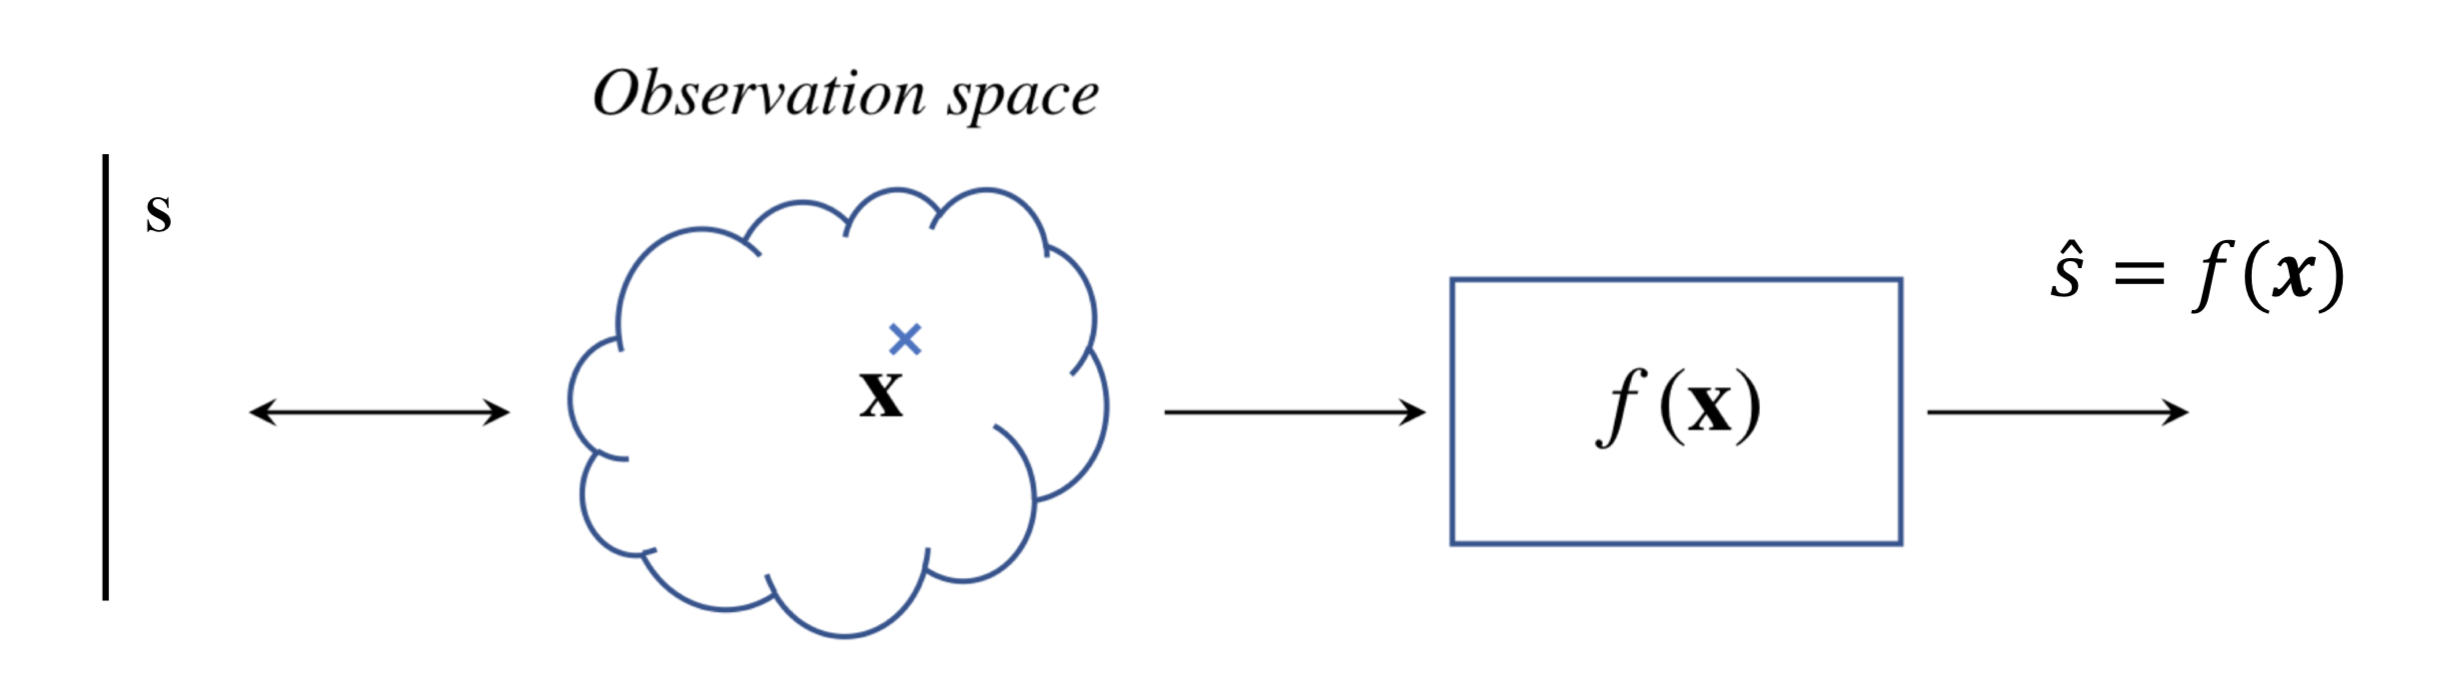
\includegraphics[width=10cm]{Figures//estimation_overview.png}
\end{center}
\caption{Diagram block of estimation problems.\label{fig:est_overview}}
\end{figure}

\textcolor{blue}{The estimator's performance is evaluated by how well $\hat{S}$ approximates $S$, typically using a predefined cost function (or, alternatively, a reward function) that quantifies the estimation error. A well-designed estimator seeks to minimize the expected cost (or to maximize the expected reward). There are two primary tasks in estimation problems:
\begin{itemize}
\item Analysis: given an estimator, assess its performance based on statistical criteria.
\item Design: find an estimator $f()$ that optimizes a predefined performance goal.
\end{itemize}
}

%%%%%%%%%%%%%%%%%%%%%%%%%%%%%%
\subsection{\textcolor{blue}{Probability model}}
\label{subsec:statistical_info}

The statistical relation between the observations and the target variable is described by the {\bf joint} probability density function (pdf), $p_{{\bf X},S}({\bf x},s)$, or some distribution related to it. The joint pdf can be factorized as \textcolor{blue}{a product} of conditional and marginal pdfs:
\begin{align}
p_{{\bf X},S}({\bf x},s) = p_{{\bf X}| S}({\bf x}| s) \cdot p_S(s) 
                         = p_{S|{\bf X}}(s|{\bf x}) \cdot p_{\bf X}({\bf x}) 
\end{align}

In the context of estimation theory, these factors receive specific names:

%%%%%%%%%%%%%%%
\begin{itemize}
\item The {\bf likelihood} of $S=s$ for observation ${\bf x}$, $p_{{\bf X}|S}({\bf x}|s)$: it characterizes the generation of observations for each value of the target variable.
\item The {\bf prior (or \textit{a priori}) distribution}  of $S$, $p_S(s)$: it describes how much is known (or unknown) about the target variable before observing ${\bf X}$. 
\item The {\bf posterior (or \textit{a posteriori}) distribution} of $S$ given ${\bf X}={\bf x}$, $p_{S|{\bf X}}(s|{\bf x})$: it describes the knowledge (or the uncertainty) about $S$ after observing ${\bf X}$.
\item The {\bf evidence} or marginal distribution of ${\bf X}$, $p_{{\bf X}}({\bf x})$.
\end{itemize}
%%%%%%%%%%%%%

\textcolor{blue}{The information available to design the estimator may depend on the application. In some cases, the likelihood function is known, because it can be related to the physical generative process of the observations. If additionally}, a prior distribution is available, the design can be grounded on the posterior distribution $p_{S|{\bf X}}(s|{\bf x})$, which can be calculated by means of Bayes' Theorem,
\begin{equation}
p_{S|{\bf X}}(s|{\bf x}) 
	= \frac{p_{{\bf X},S}({\bf x},s)} {p_{\bf X}({\bf x})} 
	= \frac{p_{{\bf X}|S}({\bf x}|s) p_S(s)}
	       {\int p_{{\bf X}|S}({\bf x}|s') p_S(s') ds'}
\end{equation}


%%%%%%%%%%%%%%%%%%%%%%%%%%%%%%%%%%%%%%%%%%%%%%%%%%%
\subsection{Cost functions for estimation problems}
\label{subsec_funcion_coste}

The evaluation and design of an estimator require some objective criteria. In some cases, we will consider that this criterion materializes in the form of a {\bf cost function} whose value we seek to minimize. %We note, however, that there are design strategies that fall outside of this approach, such as the direct maximization of some probability function.

A cost function $c(s,\hat s)$ is any measure of the discrepancy between the target variable and the estimation. It is generally non-negative, $c(s,\hat s) \geq 0$, with equality for $s = \hat s$. \textcolor{blue}{Some cost functions} can be expressed as a function of the estimation error $e= s-\hat s$ and we will write\footnote{Note that the cost function is denoted with a lowercase letter, $c$, because it is a deterministic function, i.e., for fixed values of $s$ and $\hat s$ the cost always takes the same value. However, as with the estimation function, the application of that function to random variables will result in another random variable, i.e., $C = c(S,\hat S)$.} $c(s,\hat s) = c(s - \hat s) = c(e)$. Some examples are:
\begin{itemize}
\item \textcolor{blue}{Square error}: $c(e) = e^2$.
\item \textcolor{blue}{Absolute error}: $c(e) = |e|$.
\item Relative \textcolor{blue}{square} error: $c(s,\hat s) = \frac{(s-\hat{s})^2}{s^2}$
\item Cross Entropy: $c(s,\hat s) = - s \ln \hat s - (1-s) \ln (1-\hat s)$, for $s,\hat{s}\in [0,1]$
\end{itemize}

Since the target variable is unknown, the prediction cannot be computed by directly minimizing the cost $c(s, \hat s)$, and we have to work with expectations. The expected value of the cost is usually referred as the {\bf risk} of an estimator $\hat{s}=f({\bf x})$:
\begin{align}
\label{Est:risk_def}
R_f = \EE\{c(S,\hat S)\} 
    & = \int_{\bf x} \int_s c(s,f({\bf x})) p_{S,{\bf X}}(s,{\bf x}) ds d{\bf x}
\end{align}
By the \textit{Law of Large Numbers}, this is the average cost we can expect from a given estimator, after a large number of predictions.

The {\bf conditional risk} is the conditional mean for a given observation
\begin{align}
\label{Est:cond_risk}
R(\hat s, {\bf x}) = \EE\{c(S, \hat s) |{\bf x}\} 
           & = \int_s c(s,\hat s) p_{S|{\bf X}}(s|{\bf x}) ds
\end{align}

%%%%%%%%%%%%%%%
\begin{example}[Evaluation of estimators 1]
\label{CalculoECM}
Given the joint distribution
\begin{equation}
p_{S,X}(s,x) = \left[
\begin{array}{ll}
\frac{1}{x}, & \qquad 0 \le s \le x ~~{\rm and}~ 0 < x \le 1 \\
0,           & \qquad \text{otherwise}
\end{array}
\right.,
\end{equation}
consider the estimators $\hat{S}_1 = \frac{1}{2}X$ and $\hat{S}_2 = X$. Which is the best estimator from the point of view of the \textcolor{blue}{square error}? To find out, we'll calculate the risk (i.e. the mean \textcolor{blue}{square error}) for both estimators.
Knowing that, for any $w$,
\begin{align}
R &=\mathbb{E}\{(S-wX)^2\}   
   = \int_0^1 \int_0^x (s-wx)^2 p_{S,X}(s,x) ds dx   
   = \int_0^1 \int_0^x (s-wx)^2 \frac{1}{x}ds dx   \nonumber\\
  &= \int_0^1 \left(\frac{1}{3} - w  + w^2 \right) x^2 dx  
   = \frac{1}{3}\left(\frac{1}{3} - w  + w^2 \right) 
\end{align}
Taking $w=1/2$ and $w=1$ we get, respectively, the risks
\begin{align}
R_1  = \EE\left\{(S-\hat{S}_1)^2\right\} 
	&= \EE\left\{\left(S-\frac12 X\right)^2\right\}   
     = \frac{1}{3}\left(\frac{1}{3} - \frac{1}{2}  + \frac{1}{4} \right)
     = \frac{1}{36} \\
R_2  = \EE\{(S-\hat{S}_2)^2\} & = \EE\{(S-X)^2\}   
 = \frac{1}{3}\left(\frac{1}{3} - 1  + 1 \right) = \frac{1}{9}
\end{align}
Therefore, from the point of view of the square error, $\hat{S}_1$ is a better estimator than $\hat{S}_2$.
\end{example}
%%%%%%%%%%%%%

%%%%%%%%%%%%%%%%%%%%%%%%%%%%%%%%%%%%%%%%%%%
\begin{example}[Evaluation of estimators 2]
Assume that $S$ is a random variable of mean 0 and variance 1, and $X$ is a noisy observation of $S$,
\begin{equation}
X = S + T
\end{equation}
where $T$ is a Gaussian random variable, independent of $S$, with mean $0$ variance $v$. We will compute the risk for the estimator $\hat{S} = X$ and different cost functions. For the \textcolor{blue}{square error}:
\begin{equation}
\EE\{(S-\hat{S})^2\} = \EE\{(S-X)^2\} = \EE\{T^2\} = v
\end{equation}
For the absolute error
\begin{align}
\EE\{|S-\hat{S}|\}
    &= \EE\{|T|\} 
     = \int_{-\infty}^{\infty} |t| \frac{1}{\sqrt{2\pi v}}\exp\left(-\frac{t^2}{2v}\right)dt 
\nonumber\\
    &= 2 \int_{0}^{\infty} t \frac{1}{\sqrt{2\pi v}}\exp\left(-\frac{t^2}{2v}\right)dt 
     = \sqrt{\frac{2v}{\pi}}
\end{align}
\end{example}
%%%%%%%%%%%%%%


%%%%%%%%%%%%%%%%%%%%%%%%%%%%%%
\subsection{Bias and Variance}
\label{subsec.bias_variance}

The performance of an estimator $\hat{S} = f(\mathbf{X})$ is often evaluated using two key quantities: \textit{bias} and \textit{variance}. These can be defined in both \textit{conditional} and \textit{unconditional} forms, depending on whether they are measured for a specific target variable or not.

%%%%%%%%%%%%%%%%%%
\begin{definition}[Conditional Bias]
The \textit{conditional bias} of an estimator $\hat{S}$ given that $S = s$ is defined as
\begin{align}
\text{bias}\{\hat{S} | S=s\} = \EE\{\hat{S} | S=s\} - s.
\end{align}
\end{definition}
%%%%%%%%%%%%%%%%

The conditional bias quantifies the expected deviation of the estimate from the true value of the target variable, $s$. 

%%%%%%%%%%%%%%%%%%
\begin{theorem}[Bias-Variance decomposition]
For any estimator, $\hat{S}$ of random variable $S$, the conditional mean square error can be decomposed as
\begin{align}
\EE\{(\hat{S}-S)^2|S=s\} = {\rm bias}^2\{\hat{S} | S=s\} + {\rm var}\{\hat{S} | S=s\}
\label{eq:biasvar}
\end{align}
\end{theorem}
%%%%%%%%%%%%%


\begin{proof}

Since, for any random variable, $V$, $\EE\{V^2\} = \EE\{V\}^2 + {\rm var}\{V\}$, taking $V=S-\hat{S}$, and conditioning over $S=s$, we get
\begin{align}
\EE\{(\hat{S}-S)^2|S=s\} 
	&= \EE\{\hat{S}-S|S=s\}^2 + {\rm var}\{\hat{S}-S|S=s\}   \nonumber\\
	&= {\rm bias}^2\{\hat{S} | S=s\} + {\rm var}\{\hat{S}|S=s\} 
\end{align}
\end{proof}

The bias-variance decomposition highlights a major tradeoff in estimation:
\begin{itemize}
\item Low-bias estimators tend to have high variance, leading to unstable predictions.
\item Low-variance estimators may introduce \textbf{bias} to improve stability.
\end{itemize}
y
Note that, in the above expressions, the bias, variance and mean square error are conditioned over a specific value of the target variable. We can extend these definitions to measures defined from unconditional means:

%%%%%%%%%%%%%%%%%%
\begin{definition}[Unconditional Bias]
The \textit{unconditional bias} of an estimator $\hat{S}$ of a random variable $S$ is
\begin{align}
\text{bias}\{\hat{S}\} = \EE\{\hat{S}\} - \EE\{S\}.
\end{align}
\end{definition}
%%%%%%%%%%%%%%%%

A similar unconditional bias-variance decomposition can obtained, that is given by
\begin{align}
\EE\{(\hat{S}-S)^2\} 
	&= \EE\{\hat{S}-S\}^2 + {\rm var}\{\hat{S}-S|S=s\}   \nonumber\\
	&= {\rm bias}^2\{\hat{S}\} + {\rm var}\{\hat{S}-S\} 
\end{align}

If $\text{bias}\{\hat{S} | S = s\} = 0$ for all $s$, the estimator is said to be \textit{conditionally unbiased}. If $\text{bias}\{\hat{S}\} = 0$, it is \textit{unbiased in the Bayesian sense}, meaning that its expected value matches the prior mean of $S$.


%Understanding both \textit{conditional} and \textit{unconditional} bias/variance is crucial when analyzing estimator performance, particularly when discussing the \textbf{Cramér-Rao Bound (CRB)} and the \textbf{Bayesian Cramér-Rao Bound (BCRB)}, where these distinctions play a key role.

%%%%%%%%%%%%%%%%%%%%%%%%%%%%%%
\section{Design of estimators}
%%%%%%%%%%%%%%%%%%%%%%%%%%%%%%

%%%%%%%%%%%%%%%%%%%%%%%%%%%%%%%%%%%%%%%%%%%%%%%
\subsection{Maximum Likelihood (ML) estimation}

The maximum likelihood estimator (ML) uses the likelihood as the reward function to be maximized:
\begin{equation}
\sML = \argmax_s p_{{\bf X}|S}({\bf x}|s)
     = \argmax_s \ln(p_{{\bf X}|S}({\bf x}|s))
\label{ec:est_ML}
\end{equation}

The ML estimator selects the value of the parameter $s$ that maximizes the likelihood of observing ${\bf x}$ when $S=s$. Loosely speaking, observing ${\bf x}$ when $S=\sML$ is less unexpected than if $S$ takes any other value. Note that $p_{{\bf X}|S}({\bf x}|s)$, which is a density function over random variable ${\bf X}$, is not maximized with respect to ${\bf x}$, but $s$. 
% Note that in the estimator definition alternatively includes  the use of the logarithm function (or some other with similar properties) and its use does not affect in any case the value resulting from maximization.

%%%%%%%%%%%%%%%
\begin{example}[ML Estimation]
\label{ex:est_ML_varaleat}

We want to \textcolor{blue}{compute the ML estimate of a random variable $S$ given observation $X$. The likelihood function} is given by
\begin{equation}
p_{X|S}(x|s) = \frac{2 x}{(1 - s)^2},\qquad 0 \le x \le 1-s,\quad 0 \le s \le 1
\label{eq:est_exml}
\end{equation}
\textcolor{blue}{and it is represented in Figure \ref{fig:est_ML_caso1}(a) as a function of $x$, for a specific value of $s$. Note that the likelihood function is a conditional density function of the random variable $X$. However, since we aim to estimate $S$, it may be more useful to represent the likelihood as a function of $s$, for a given observation $x$, as shown in Fig.\ref{fig:est_ML_caso1}(b),\footnote{Note that the integral with respect to $s$ of $p_{X|S}(x|s)$ will not generally be equal to one, since the likelihood function is not a probability density function of the target variable $S$.}. This representation suggests that the ML estimator is
$$\hat s_{\text{ML}} = 1 - x$$
which can be corroborated by inspecting \eqref{eq:est_exml}, which shows that the likelihood increases with $s$. If we apply the estimation function to random variable $X$ instead of a specific value, we have
$$\hat S_{\text{ML}} = 1 - X$$}

% We avoid using figure here, because the example is framed, and no float environments are allowed.
\centering
\begin{tabular}{cc}
\includegraphics[width=6cm]{Figures/px_s_funcionx.png} &
\includegraphics[width=6cm]{Figures/px_s_funcions.png}\\
   (a) & (b)
\end{tabular}
\captionof{figure}{Representation of the likelihood distribution of the example \ref{ex:est_ML_varaleat} as a function of $x$ and $s$.}
\label{fig:est_ML_caso1}

%%%%%%%%%%%%%%%
%\begin{figure}[h]
%  \begin{center}
%  \begin{tabular}{cc}
%    \includegraphics[width=6cm]{Figures//px_s_funcionx.png} &
%    \includegraphics[width=6cm]{Figures//px_s_funcions.png} \\
%    (a) & (b)
%  \end{tabular}
%    \caption{Representation of the likelihood distribution of the example \ref{ex:est_ML_varaleat} as a function of $x$ and $s$.}
%    \label{fig:est_ML_caso1}
%  \end{center}
%\end{figure}
%%%%%%%%%%%%%

\end{example}
%%%%%%%%%%%%%

Note that the second equality in \eqref{ec:est_ML} states that the maximization of the likelihood is equivalent to the maximization of its logarithm (the \textbf{log-likelihood} function). Since the logarithm function is strictly increasing, $p_{{\bf X}|S}({\bf x}|s_1) > p_{{\bf X}|S}({\bf x}|s_2)$ implies $\ln(p_{{\bf X}|S}({\bf x}|s_1)) > \ln(p_{{\bf X}|S}({\bf x}|s_2))$) and, thus, the logarithm does not alter the outcome of the maximization. The logarithm is \textcolor{blue}{useful to simplify the optimization when} the likelihood is a product of several factors or an exponential function, as it will transform products into sums and an exponential into the exponents. 

Note that the maximum likelihood does not need any probability model about the target variable, $S$, which is treated as a deterministic parameter.


%%%%%%%%%%%%%%%%%%%%%%%%%%%%%%%%%%%%%%%%%%%%%%%%%%
\subsection{Maximum a posteriori (MAP) estimation}

We define the maximum a posteriori (MAP) estimator as the mode of the posterior distribution, that is
\begin{equation}
\hat s_{\text{MAP}} = \argmax_{s} p_{{S|\bf X}}(s|{\bf x})
                    = \argmax_{s} \ln(p_{{S|\bf X}}(s|{\bf x}))
                   \label{ec:est_MAP}
\end{equation}

Using the definition of conditional pdf and Bayes' rule, it is easy to see that the MAP estimator can be altenatively computed as
\begin{align}
\label{eq:est_smap2}
\hat s_{\text{MAP}} 
	&= \argmax_{s} p_{{S,\bf X}}(s,{\bf x})   \\
\label{eq:est_smap3}
    &= \argmax_{s} \{p_{{\bf X}|S}({\bf x}|s) p_S(s)\}
\end{align}

Eq. \eqref{eq:est_smap3} demonstrates that the MAP estimator seeks to maximize the likelihood function, modulated by the prior distribution. This integration of the prior distribution allows the MAP estimator to incorporate existing knowledge or assumptions about the target $S$ before observing the data, ${\bf x}$. When the prior distribution is uniform across the \textcolor{blue}{domain} of $S$, the distinction between the MAP and ML estimators vanishes, as the MAP estimator effectively reduces to the ML estimator.

However, when the prior distribution is not uniform, the MAP estimator is biased towards values of the target variable with higher prior probabilities. This shift illustrates the MAP estimator's sensitivity to prior knowledge.

Beyond their mathematical formulations, the MAP and ML estimators embody fundamentally different inference philosophies. The ML estimator optimizes the likelihood function, which models the probability of the observed data under various values of the target, treating $s$ as a fixed but unknown parameter. This approach aligns with the \textbf{frequentist paradigm}, which interprets probability as the long-run frequency of events and does not incorporate prior information about $S$.

Conversely, the MAP estimator embraces a \textbf{Bayesian framework}, treating the target as a random variable. This perspective allows the incorporation of prior knowledge or beliefs about $S$ through the prior distribution, $p_S(s)$, and the posterior distribution, $p_{{S|\bf X}}(s|{\bf x})$, updates this knowledge based on new evidence from the data. The Bayesian approach, therefore, provides a probabilistic framework for updating beliefs about uncertain parameters in light of new data.

%%%%%%%%%%%%%%%
\begin{example}[\textcolor{blue}{MAP estimation}]
\textcolor{blue}{Given the posterior density}  
\begin{equation}
p_{S|X}(s|x) = \frac{1}{x^2} s \exp\left(-\frac{s}{x}\right), \qquad  x\ge 0,\quad s \ge 0
\end{equation}
the MAP estimator can be computed by maximizing
\begin{equation}
\ln(p_{S|X}(s|x)) = -2\ln(x) + \ln(s)-\frac{s}{x}, \qquad  x\ge 0,\quad s \ge 0,
\end{equation}
Since $\ln(p_{S|X}(s|x))$ tends to $-\infty$ around $s=0 $ and $s=\infty$, its maximum must be at some intermediate point with zero derivative:
\begin{equation}
\left.\frac{\partial}{\partial s} \ln p_{S|X}(s|x)\right|_{s=\sMAP} 
	= \frac{1}{\sMAP} - \frac{1}{x} 
	= 0, \qquad  x\ge 0, \quad s \ge 0.
\end{equation}
Therefore,
\begin{equation}
\sMAP = x
\end{equation}
\end{example}   %\vspace{0.4cm}
%%%%%%%%%%%%%

%%%%%%%%%%%%%%%%%%%%%%%%%%%%%%%%%%%%
\subsection{Minimum risk estimators}

\textcolor{blue}{On major drawback of the MAP estimator is that a high posterior density at a given point does not necessarily mean that the estimated value is likely to be close to the true parameter, as the example in Fig. \ref{fig:map_paradox} shows, where the MAP estimate lies in a region with low probability. This motivates the application of other Bayesian estimators that take into account the cost of large deviations from the true parameter.}

%%%%%%%%%%%%%%
\begin{figure}[h]
\begin{center}
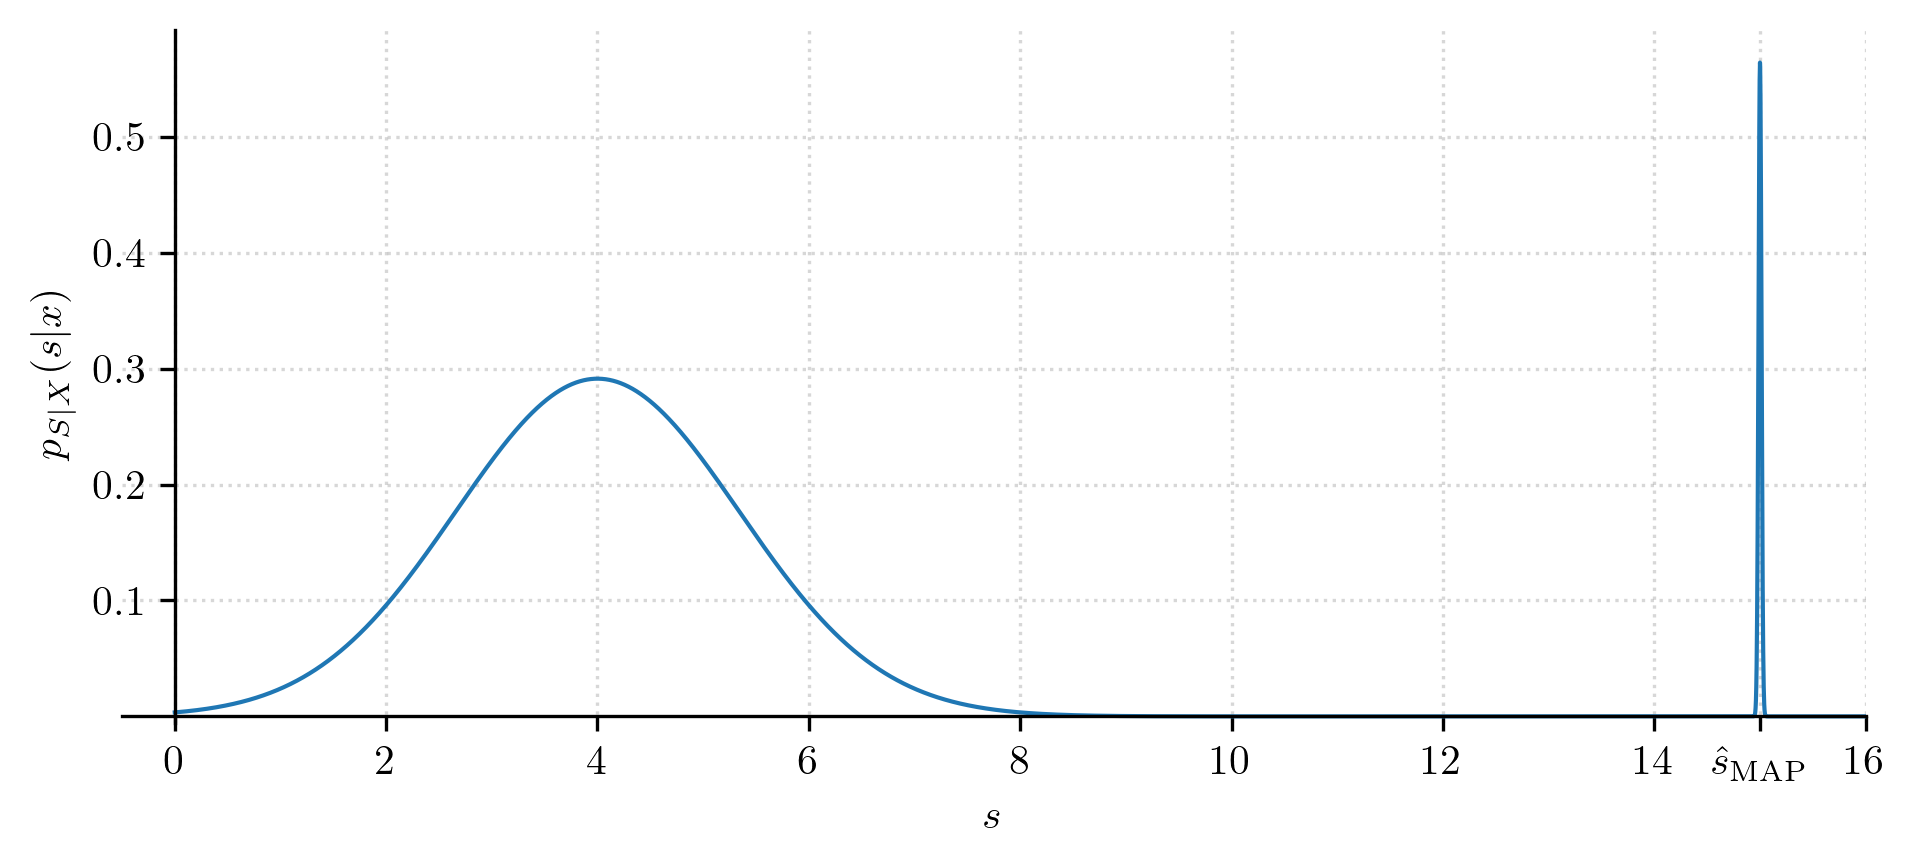
\includegraphics[width=14cm]{Figures//et_smapexample.png} 
\caption{A visual example of a posterior distribution, where the MAP estimate can be far from the true value of the target parameter with high probability.}
\label{fig:map_paradox}
\end{center}
\end{figure}
%%%%%%%%%%%%

\textcolor{blue}{The Bayesian estimator for a cost function $c(S,\hat S)$ is the one minimizing the risk \eqref{Est:risk_def}. Applying the total expectation theorem, the risk of estimator $\hat s= f({\bf x})$ can be expressed as}
\begin{align}
\label{ec:coste_medio}
R_f = \EE\{c(S,\hat S)\} 
  & = \int_{\bf x} \EE\{c(S,\hat s)|{\bf X} = {\bf x} \} 
               p_{\bf X}(\bf x) d{\bf x}
\end{align}
where $\hat s= f({\bf x})$. That is, the risk is the integral of the conditional risk, and, thus, the estimator minimizing \textcolor{blue}{$R_f$ should minimize} the conditional risk for each observation ${\bf x}$,
\begin{equation}
\label{ec:est_bayesiano}
{\hat s}^* = \argmin_{\hat s}\;\EE\{c(S,\hat s)|{\bf X} = {\bf x} \}
\end{equation}


%%%%%%%%%%%%%%%
\begin{example}[Calculation of a minimum mean square error estimator]
\label{CalculoECM2}
Following the example \ref{CalculoECM}, we can calculate the posterior distribution of $S$ through
\begin{equation}
p_{S|X}(s|x) = \frac{p_{S,X}(s,x)}{p_X(x)}. 
\end{equation}
Knowing that
\begin{equation}
p_{X}(x) = \int_0^1 p_{S,X}(s,x) ds = \int_0^x \frac{1}{x} ds = 1,   \qquad 0\le x\le 1
\end{equation}
we obtain
\begin{equation}
p_{S|X}(s|x) = \left[
\begin{array}{ll}
\frac{1}{x}, & \qquad 0<s<x<1 \\
0,           & \qquad \text{otherwise}
\end{array}
\right.
\end{equation}
The conditional risk will be given by
\begin{align}
\mathbb{E}\{c(S,\hat s)|X=x\} 
   &= \mathbb{E}\{(S-\hat s)^2|X=x\} \nonumber\\
   &= \int_0^1 (s-\hat{s})^2 p_{S|X}(s|x) ds   \nonumber\\
   &= \frac{1}{x} \int_0^x (s-\hat{s})^2 ds  
    = \frac{1}{x} \left(\frac{(x-\hat{s})^3}{3} + \frac{\hat{s}^3}{3} \right)    \nonumber\\
   &= \frac{1}{3}x^2 - \hat{s} x + \hat{s}^2. 
\label{Est:ECMsx}
\end{align}

As a function of $\hat{s}$, conditional risk is a second-degree polynomial, whose minimum can be calculated through differentiation. Since
\begin{align}
\frac{d}{d\hat{s}} \mathbb{E}\{c(S,\hat s)|X=x\} 
   &= - x + 2 \hat{s} ,
\end{align}
the Bayesian estimator associated with the \textcolor{blue}{square error} is
\begin{equation}
\label{eq:sopt_halfx}
\hat{s}^* = \frac{1}{2}x,
\end{equation}
which matches the estimator $\hat{S}_1$ from the example \ref{CalculoECM}. Therefore, $\hat{S}_1$ is the best possible estimator from the point of view of the mean square error.
\end{example}\vspace{0.4cm}
%%%%%%%%%%%%%

%\newpage

%%%%%%%%%%%%%%%%%%%%%%%%%%%%%%%%%%%%%%%%%%%%%%%%%
\section{Common Bayesian estimators}
%%%%%%%%%%%%%%%%%%%%%%%%%%%%%%%%%%%%%%%%%%%%%%%%%

\textcolor{blue}{In this section we derive some of the most widely used Bayesian estimators, starting from different choices of the loss function.}


%%%%%%%%%%%%%%%%%%%%%%%%%%%%%%%%%%%%%%%%%%%%%%%%%%%%%%%
\subsection{Minimum Mean Squared Error estimator (MSE)}

The minimum mean squared error (MSE) estimator is the Bayesian estimator associated with the cost function $c(e) = e^2 = (s-\hat s)^2$, and therefore is given by 
\begin{align}
\label{ec:coste_medio_cuadratico}
\sMSE 
  & = \argmin_{\hat s} \; \EE\{c(S,\hat s)|{\bf X} = {\bf x} \}   \nonumber\\
  & = \argmin_{\hat s} \; \EE\{(S-\hat s)^2|{\bf X} = {\bf x} \}
\end{align}

Figure \ref{fig:estimador_cuadratico} illustrates the minimum MSE estimation problem. The risk can be obtained by integrating (with respect to $s$) the product of the square error and the posterior pdf of $S$. The argument for minimization is $\hat s$, which allows shifting the graph corresponding to the cost function (represented with discontinuous stroke) so that the result of that integral is minimal.

%%%%%%%%%%%%%%
\begin{figure}[th]
  \begin{center}
    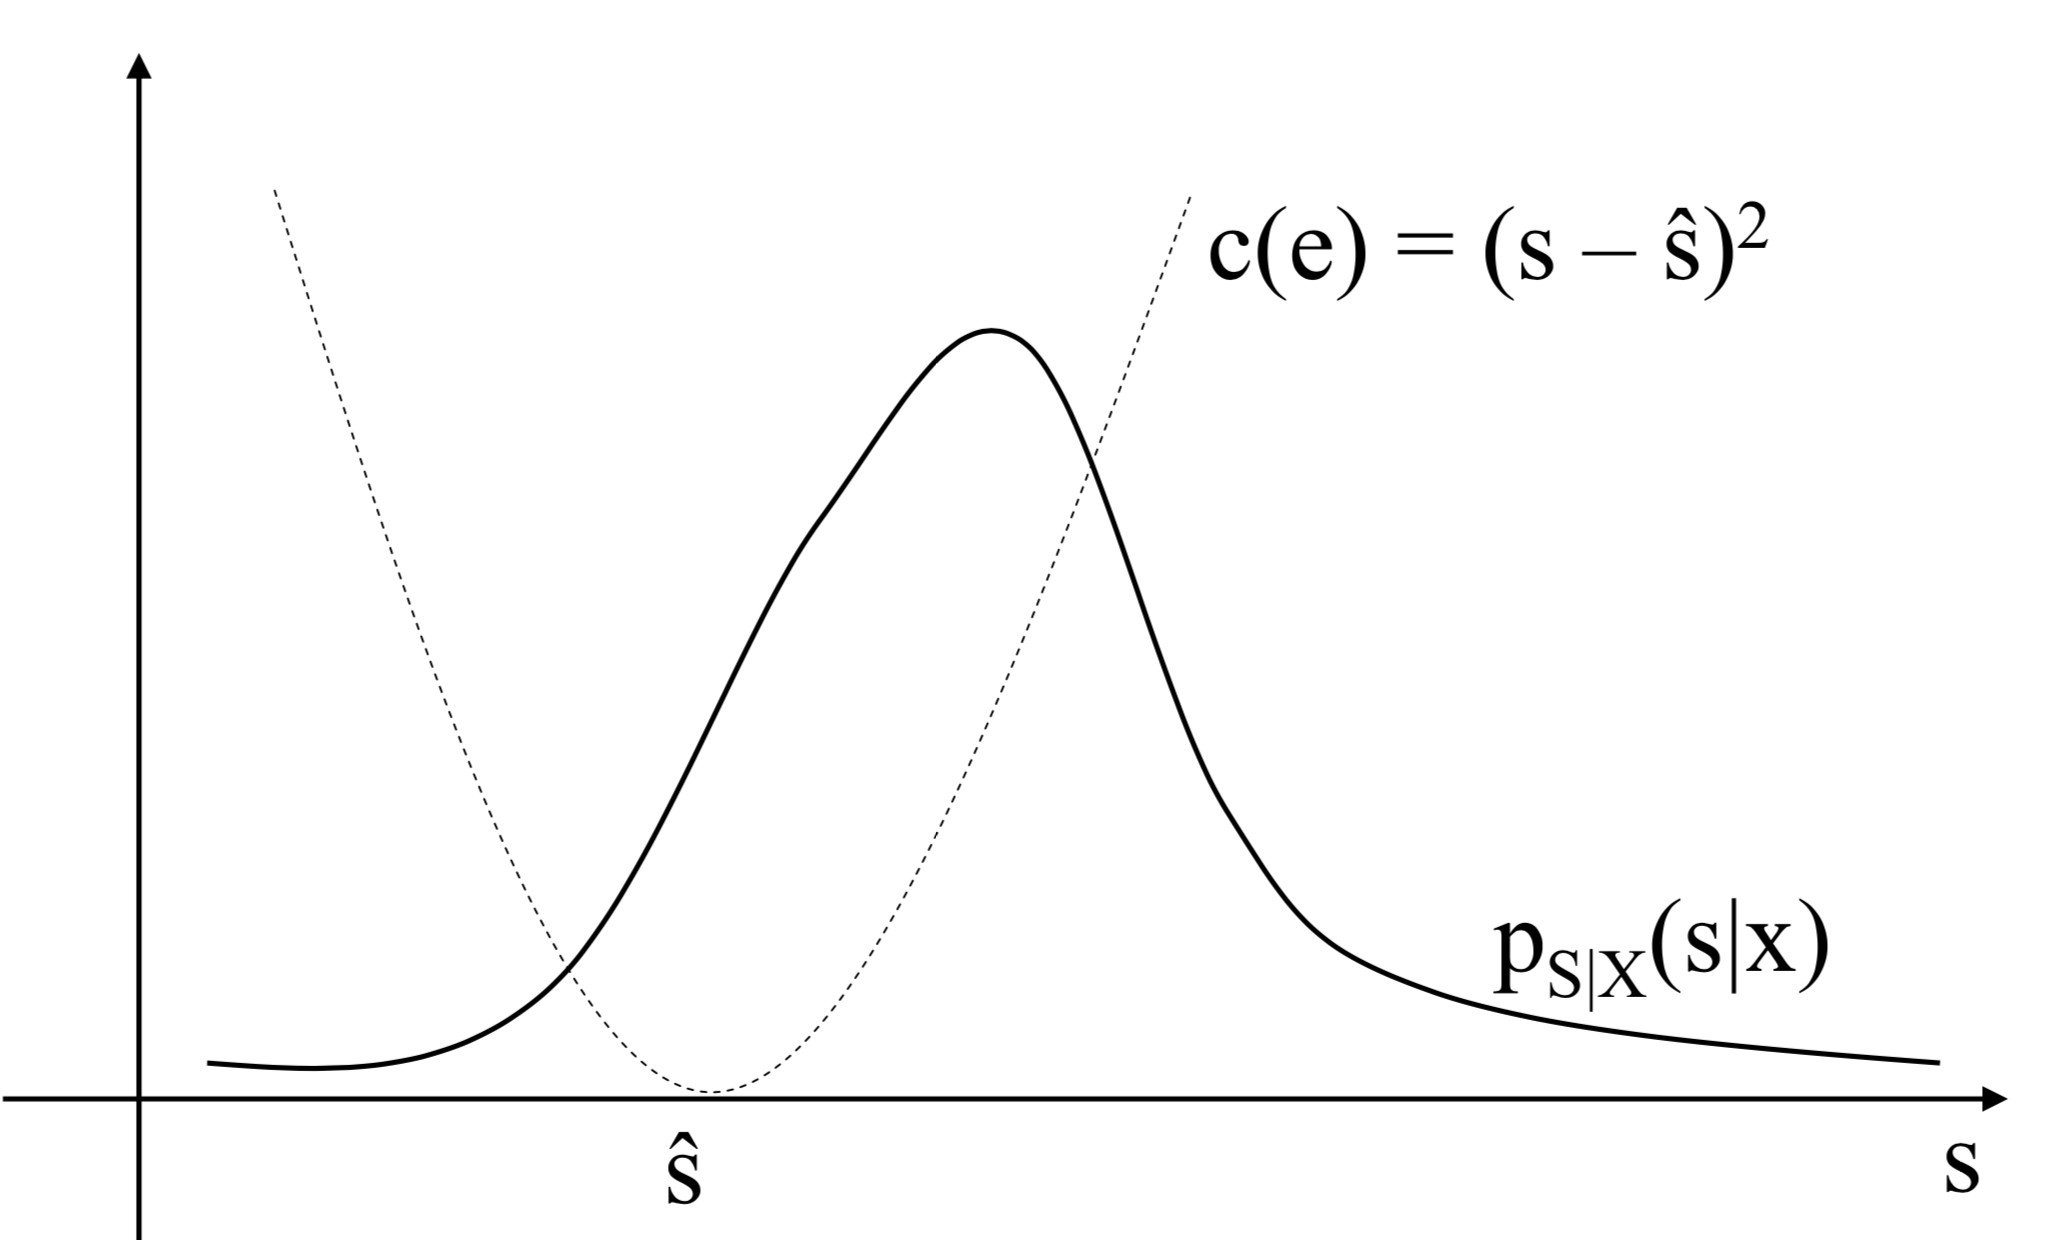
\includegraphics[width=7cm]{Figures//estimador_cuadratico.png}
    \caption{Graphical representation of the process of calculating the posterior mean for a generic value $\hat{s}$.}
    \label{fig:estimador_cuadratico}
  \end{center}
\end{figure}
%%%%%%%%%%%%

For the square error, the conditional risk in \eqref{ec:coste_medio_cuadratico} becomes
\begin{align}
\label{ec:gen_mse2}
\EE\{(S-\hat s)^2|{\bf X} = {\bf x} \}
    = \EE\{S^2|{\bf X} = {\bf x} \}
    - 2\EE\{S|{\bf X} = {\bf x} \} \hat s
    + \hat s^2
\end{align}
This is a second-degree polynomial that can be minimized by differentiation to get
\begin{framed}
\begin{equation}
\label{ec:estimador_MSE_final}
\sMSE = \EE\{S|{\bf X} ={\bf x}\} = \int s \cdot p_{S|{\bf X}}(s|x) ds
\end{equation}
\end{framed}

In other words, the minimum MSE estimator of $S$ is the posterior mean of $S$ given $\bf X$.

%%%%%%%%%%%%%%%
\begin{example}[MSE estimator]
According to \eqref{ec:estimador_MSE_final}, minimum mean squared error estimator obtained in \ref{CalculoECM} can alternatively be derived as follows

\begin{align}
\label{ec:estimador_MSE_final2}
\hat s_{\text{MSE}} = \int_0^1 s p_{S|X}(s|x) ds   
   = \int_0^x \frac{s}{x} ds 
   = \frac{1}{2} x
\end{align}
which is consistent with \eqref{eq:sopt_halfx}.
\end{example}\vspace{0.4cm}
%%%%%%%%%%%%%



%%%%%%%%%%%%%%%%%%%%%%%%%%%%%%%%%%%%%%%%%%%%%%%%%%%%%
\subsection{Minimum Mean Absolute Deviation Estimator (MAD)}

When the cost is the absolute deviation, $c(e) = |e| = |s - \hat s|$, the minimizer of the conditional risk (which we will refer to as the Mean Absolute Deviation, or MAD, estimator), is given by
\begin{align}
\label{ec:coste_MAD}
\sMAD & = \argmin_{\hat s}\; \EE\{|S - \hat s|~|{\bf X} = {\bf x} \} = \\
	  & = \argmin_{\hat s}   \int_s |s - \hat s|\;p_{S|{\bf X}}(s|{\bf x}) ds
\end{align}
\textcolor{blue}{The computation of the conditional risk is illustrated in Fig. \ref{fig:estimador_absoluto}}. This representation also suggests the convenience of splitting the integral into two parts corresponding to the two slopes of the cost function:
\begin{align}
\EE\{|S - \hat s|~|{\bf X} = {\bf x} \} 
	=& \int_{-\infty}^{\hat s} (\hat s - s) \;p_{S|{\bf X}}(s|{\bf x}) ds
		+ \int_{\hat s}^\infty (s - \hat s) \;p_{S|{\bf X}}(s|{\bf x}) ds \\
	=& \hat s \left[  \int_{-\infty}^{\hat s} p_{S|{\bf X}}(s|{\bf x}) ds 
				    - \int_{\hat s}^{\infty}  p_{S|{\bf X}}(s|{\bf x}) ds \right]  \nonumber\\
	 &  + \int_{\hat s}^{\infty}  s \; p_{S|{\bf X}}(s|{\bf x}) ds 
		- \int_{-\infty}^{\hat s} s \; p_{S|{\bf X}}(s|{\bf x}) ds
\end{align}

%%%%%%%%%%%%%%
\begin{figure}[t]
  \begin{center}
  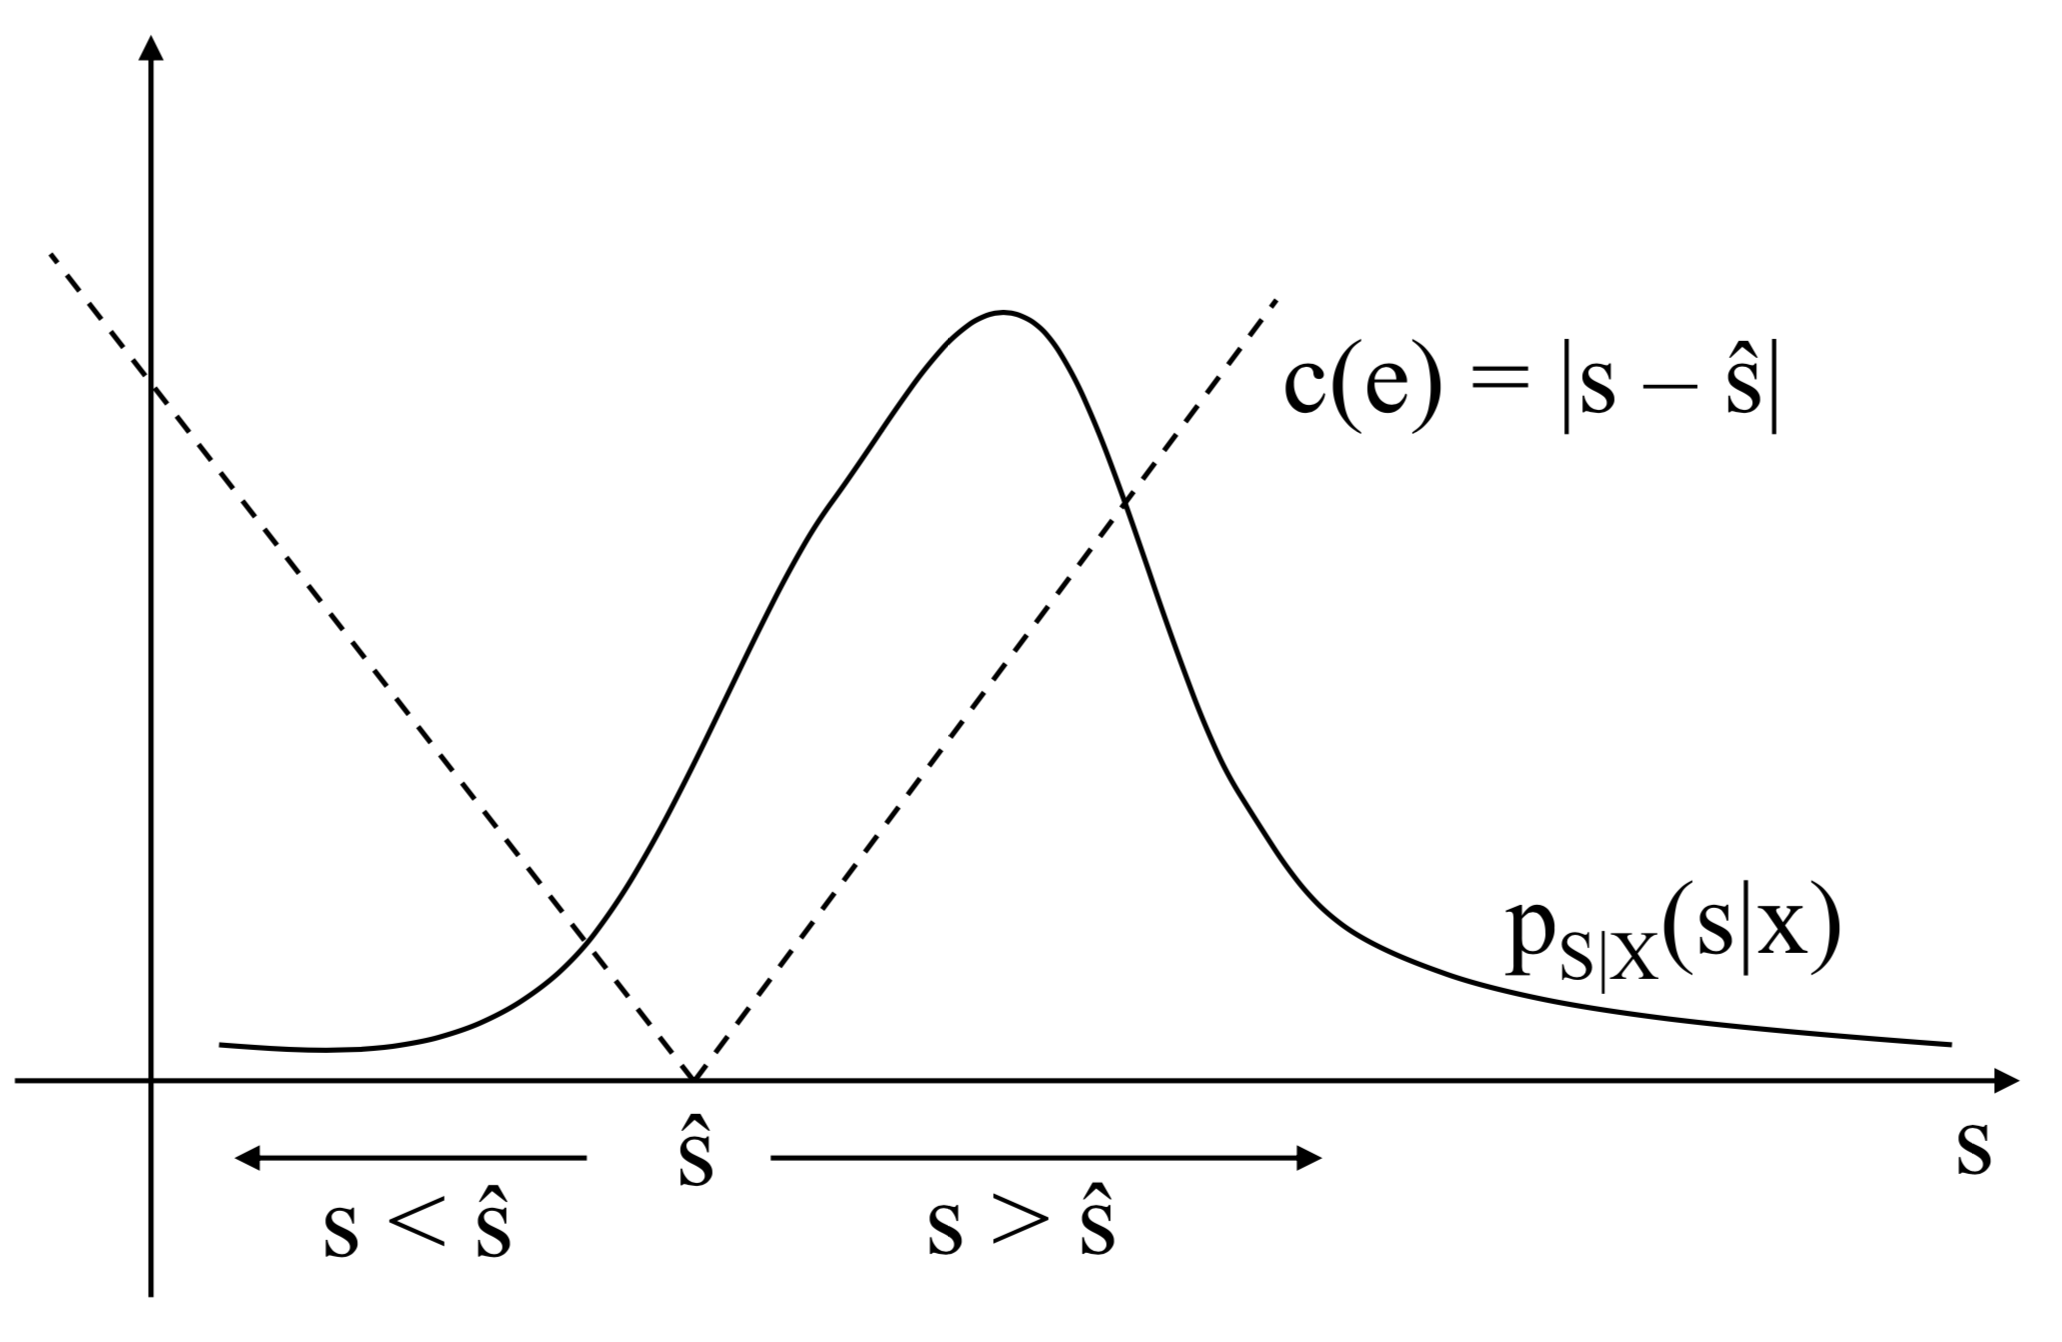
\includegraphics[width=7cm]{Figures//estimador_absoluto.png}
    \caption{Calculation of the posterior mean absolute error for a generic value $\hat s$.}
    \label{fig:estimador_absoluto}
  \end{center}
\end{figure}
%%%%%%%%%%%%

\textcolor{blue}{Applying the} fundamental theorem of calculus\footnote{$\frac{d}{d x} \int_{t_0}^x g(t) dt = g(x)$.} we can write\footnote{Strictly speaking, it is assumed here that the posterior distribution is absolutely continuous, that is, $p_{S|X}(s|x)$ does not contain singularities (i.e. points with nonzero probability mass).}
\begin{equation}
\frac{d \mathbb{E}\{|S - \hat s|~|{\bf X} = {\bf x} \}}{d \hat s} 
    = 2 F_{S|{\bf X}}(\hat s|{\bf x}) - 1
\end{equation}
where $F_{S|{\bf X}}(s|{\bf x})$ is the posterior cumulative distribution function of $S$ given ${\bf X}$. Since this derivative must vanish at the minimum, we get $F_{S|{\bf X}}(\hat s_{\text{MAD}}|{\bf x}) = 1/2$. In other words, the minimum MAD estimator is given by the median of $p_{S|{\bf X}}(s|{\bf x})$:

\begin{framed}
\begin{equation}
\label{ec:estimador_MAD_final}
\hat s_{\text{MAD}} = \text{median}\{S|{\bf X} ={\bf x}\}
\end{equation}
\end{framed}

Remember that the median of a distribution is the point that \textcolor{blue}{splits its domain} into two sets with the same probability, so the minimum MAD estimator satisfies
\begin{align}
P\{S > \sMAD |{\bf x}\} = P\{S < \sMAD |{\bf x}\}
\end{align}

In practice, this can be computed as the solution of
\begin{align}
\int_{-\infty}^{\sMAD} p_{S|{\bf X}}(s|{\bf x}) ds = \frac12
\end{align}


\begin{example}[MAD Estimator]

In the scenario of the example \ref{CalculoECM}, the posterior distribution of $S$ given $X$ is uniform between 0 and $x$, the median of which is $x/2$. Thus,
\begin{align}
\label{ec:estimador_MSE_finalej}
\sMAD = \frac{1}{2} x 
\end{align}

Note that, in this case, the MAD estimator matches the MSE obtained at \eqref{eq:sopt_halfx}. This is a consequence of the symmetry of the a posterior distribution.
\end{example}




%%%%%%%%%%%%%%%%%%%%%%%%%%%%%%%%%%%%%%
\section{Estimation with constrains}
%%%%%%%%%%%%%%%%%%%%%%%%%%%%%%%%%%%%%%


%%%%%%%%%%%%%%%%%%%%%%%%%%%%%%%%%
\subsection{General principles}

Occasionally, it might be beneficial to prescribe a specific parametric form for the estimator, denoted as $\hat S = f_{\bf w}(\bf X)$, where ${\bf w}$ represents a vector of parameters. For instance, in scenarios involving two observations, ${\bf X} = [X_1, X_2]^T$, a design constraint might necessitate limiting the search for an estimator to the family of quadratic estimators, characterized by $\hat S = w_0 + w_1 X_1^2 + w_2 X_2^2$. In such situations, the task of designing an estimator consists of identifying the optimal parameter vector ${\bf w}^*$ that minimizes the risk, while adhering to the specified constraints on the estimator structure:
\begin{align}
{\bf w}^* &= \argmin_{\bf w} \EE\{c(S,\hat S)\}
           = \argmin_{\bf w} \EE\{c(S,f_{\bf w}({\bf X}))\} \nonumber\\
          &= \argmin_{\bf w} \int_{\bf x} \int_s c(s,f_{\bf w}({\bf x})) 
                                                 p_{S,{\bf X}}(s,{\bf x}) ds d{\bf x}.
\end{align}

Restricting the estimator to a specific analytic form typically results in a higher risk than what could be achieved with a Bayesian estimator tailored to the same cost function. The exception to this rule occurs when the imposed constraints align with the optimal estimator form, essentially when the Bayesian estimator inherently fits within the specified constraints. Despite potentially incurring higher costs, practical considerations may justify opting for such constrained estimators, such as simplification in design or implementation. An exploration of this concept is presented in Section \ref{sec:est_lineal}, focusing on linear estimators that achieve minimum MSE.

%%%%%%%%%%%%%%%
\begin{example}[\textcolor{blue}{Estimator with Constraints}]
\label{CalculoECM_rest}

Continuing the example \ref{CalculoECM2}, we want to calculate the minimum MSE estimator with the form $\hat{s} = wx^2$. \textcolor{blue}{Since the conditional risk is given by \eqref{Est:ECMsx}, the risk can be computed as}
\begin{align}
\label{ec:coste_medio2}
\EE\{c(S,\hat S)\} 
   &= \int_x \EE\{c(S,\hat s)|X=x\} \;p_X(x) dx  \nonumber\\
   &= \int_x \left(\frac{1}{3}x^2 -\hat{s}x +\hat{s}^2 \right) 
                   p_X(x) dx
\end{align}
Forcing $\hat{s} = wx^2$ and taking into account that $p_X(x)=1$ for $ 0<x<1$ , we get the MSE as a function of $w$.
\begin{align}
\mathbb{E}\{c(S,wX^2)\} 
   & = \int_0^1 \left(\frac{1}{3}x^2 - wx^3 + w^2x^4 \right) dx \\
   & = \frac{1}{9} - \frac{1}{4} w + \frac{1}{5} w^2
\label{Est:ECMwx2}
\end{align}
Since the risk is a quadratic funtion of $w$, it can be optimized by differentiation, to get 
\begin{equation}
\label{eq:sopt_58}
w^* = \frac{5}{8},
\end{equation}
and therefore the estimator is $\hat{s} = \frac{5}{8}x^2$.

\end{example}\vspace{0.4cm}
%%%%%%%%%%%%%


%%%%%%%%%%%%%%%%%%%%%%%%%%%%%%%%%%%%%%%%%%%%%%%%%%%%%%%%%%%%%%%
\subsection{Linear (in the parameters) estimation of minimum MSE}
\label{sec:est_lineal}

In this section we will focus on the study of estimators that are a linear combination of variables related to the observations, using the minimization of the MSE as a design criterion. More specifically, we will consider estimators given by the general expression
{\begin{align}
\label{Est:lin_in_w}
\hat S = {\bf w}^\intercal {\bf Z}
\end{align}
where 
\begin{align}
{\bf Z}=\phi({\bf X})
\end{align}
is some known transformation of the observations. The nature of this transformation may depend on the application, but there are some cases of particular interest:
\begin{itemize}
\item \textbf{Linear estimation}: in this case, $\phi$ is the identity function, so that ${\bf Z}={\bf X}$, and the estimator a linear function of the observations
\begin{equation}
\hat S = w_0 X_0 + w_1 X_1 + \dots + w_{N-1} X_{N-1}
\end{equation}
\item \textbf{Linear estimation with independent term}: in this case, ${\bf Z}=(1, {\bf X}^\intercal)^\intercal$ and
\begin{equation}
\label{Est:blin}
\hat S = w_0 + w_1 X_0 + \dots + w_{N} X_{N-1}
\end{equation}
\item \textbf{Polynomial estimation}: the components of ${\bf Z}$ are monomials of the observational variables. For instance, for a scalar observation $X \in \mathbb{R}$, we can take ${\bf Z} = (1, X, X^2, \ldots X^M)$, for some $M>1$, and the estimation becomes an $M$-degree polynomial of the observation.
\begin{equation}
\hat S = w_0 + w_1 X + w_2 X^2 \dots + w_M X^M
\end{equation}
\end{itemize}}

{Note that in general, \textcolor{blue}{${\bf X}$ and ${\bf Z}$ may have different dimensions}. Note, also, that, despite the estimator may be a non-linear function of the observation, all estimators given by \eqref{Est:lin_in_w} are linear functions of the parameters. For this reason, we will refer to them as estimators that are \textit{linear in the parameters}.}

%where $N$ denotes the number of available observable variables, $\{X_i\}_{i=1}^N$, and $\{w_i\}_{i=0}^{N}$ are the weights that characterize the estimator. In this context, it is common to refer to the term independent of the above expression, $w_0$, as a bias term. For analytic simplicity, it is more convenient to enter the following matrix notation:
%\begin{equation}
%\hat S = w_0 + {\bf w}^T {\bf X} = {\bf w}_{\text{e}}^T {\bf X}_{\text{e}}
%\label{Est:Sestlineal}
%\end{equation}
%where ${\bf w} = [w_1,\dots,w_N]^T$ and ${\bf X} = [X_1,\dots,X_N]^T$ are the (column) vectors  of parameters and observations, respectively, and ${\bf w}_{\text{e}} = [w_0, {\bf w}^T]^T$ and ${\bf X}_{\text{e}} = [1, {\bf X}^T]^T$ are extended versions of these vectors.

By imposing a restriction on the analytic form of the estimator, linear-in-the-parameter estimators will generally obtain lower performance than the optimal Bayesian estimator. However, the interest in linear estimators is justified by their simplicity and ease of design. As we shall see, the linear estimator of minimum MSE depends exclusively on first and second-order statistical moments (means and covariances) {associated with the target variable and the transformed observation, ${\bf Z}$}.

%On the other hand, the use of linear estimators is fully justified in certain circumstances, for example when dealing with variables with Gaussian distributions, since, as we saw in the previous section, in this case the Bayesian estimator with the minimum squared mean error has a linear architecture. 


%%%%%%%%%%%%%%%%%%%%%%%%%%%%%%%%%%%%%%%%%%%%%%%%%%%%%%%%%
\subsubsection{Minimization of the {mean squared error}.}% y ecuaciones normales}

We will consider as design criteria the squared error, $c(e) = (s-\hat s)^2$, so the optimal weight vector will be the one that minimizes the MSE risk:
{\begin{equation}
{\bf w}^* 
	= \argmin_{\bf w} \; \EE\{(S - \hat S)^2\} 
    = \argmin_{\bf w}\;  \EE\{(S - {\bf w}^\intercal {\bf Z})^2\}
\end{equation}
and we will refer to the estimator associated with the weight vector as $\hat S_\text{LMSE}$: 
$$\hat S_\text{LMSE} = {{\bf w}^*}^T {\bf Z}$$}

{The MSE can be expanded as
\begin{align}
\label{Est:LMSEw}
MSE &= \EE\{(S - \hat S)^2\} = \EE\{(S - {\bf w}^\intercal {\bf Z})^2\}  \nonumber\\
    &= \EE\{S^2\} - 2 \EE\{{\bf w}^\intercal{\bf Z}S\} 
      + \EE\{\left({\bf w}^\intercal {\bf Z}\right)^2\}   \nonumber\\
    &= \EE\{S^2\} - 2 \EE\{S {\bf Z}\}^\intercal {\bf w} 
      + {\bf w}^\intercal \EE\{{\bf Z}{\bf Z}^\intercal\}{\bf w} \nonumber\\
    &= \EE\{S^2\} - 2 {\bf r}_{S{\bf Z}}^\intercal {\bf w} 
      + {\bf w}^\intercal {\bf R}_{\bf Z} {\bf w}
\end{align}
where
\begin{itemize}
\item ${\bf r}_{S{\bf Z}} = \EE\{S {\bf Z}\}$ is the \textbf{cross-correlation vector} between $S$ and ${\bf Z}$
\item ${\bf R}_{\bf Z}=\EE\{{\bf Z}{\bf Z}^\intercal\}$ is the \textbf{autocorrelation matrix} of ${\bf Z}$.
\end{itemize}
Thus, the MSE is a second-degree polynomial in ${\bf w}$}. This is illustrated in Figure \ref{fig:linear_est_error_surface}, which depicts the error surface in a case with two observations. Being the function to minimize quadratic in weights (minimization argument), the error surface will take the form of a $N$ dimensional paraboloid. 
%%%%%%%%%%%%%%
\begin{figure}[htb]
  \begin{center}
  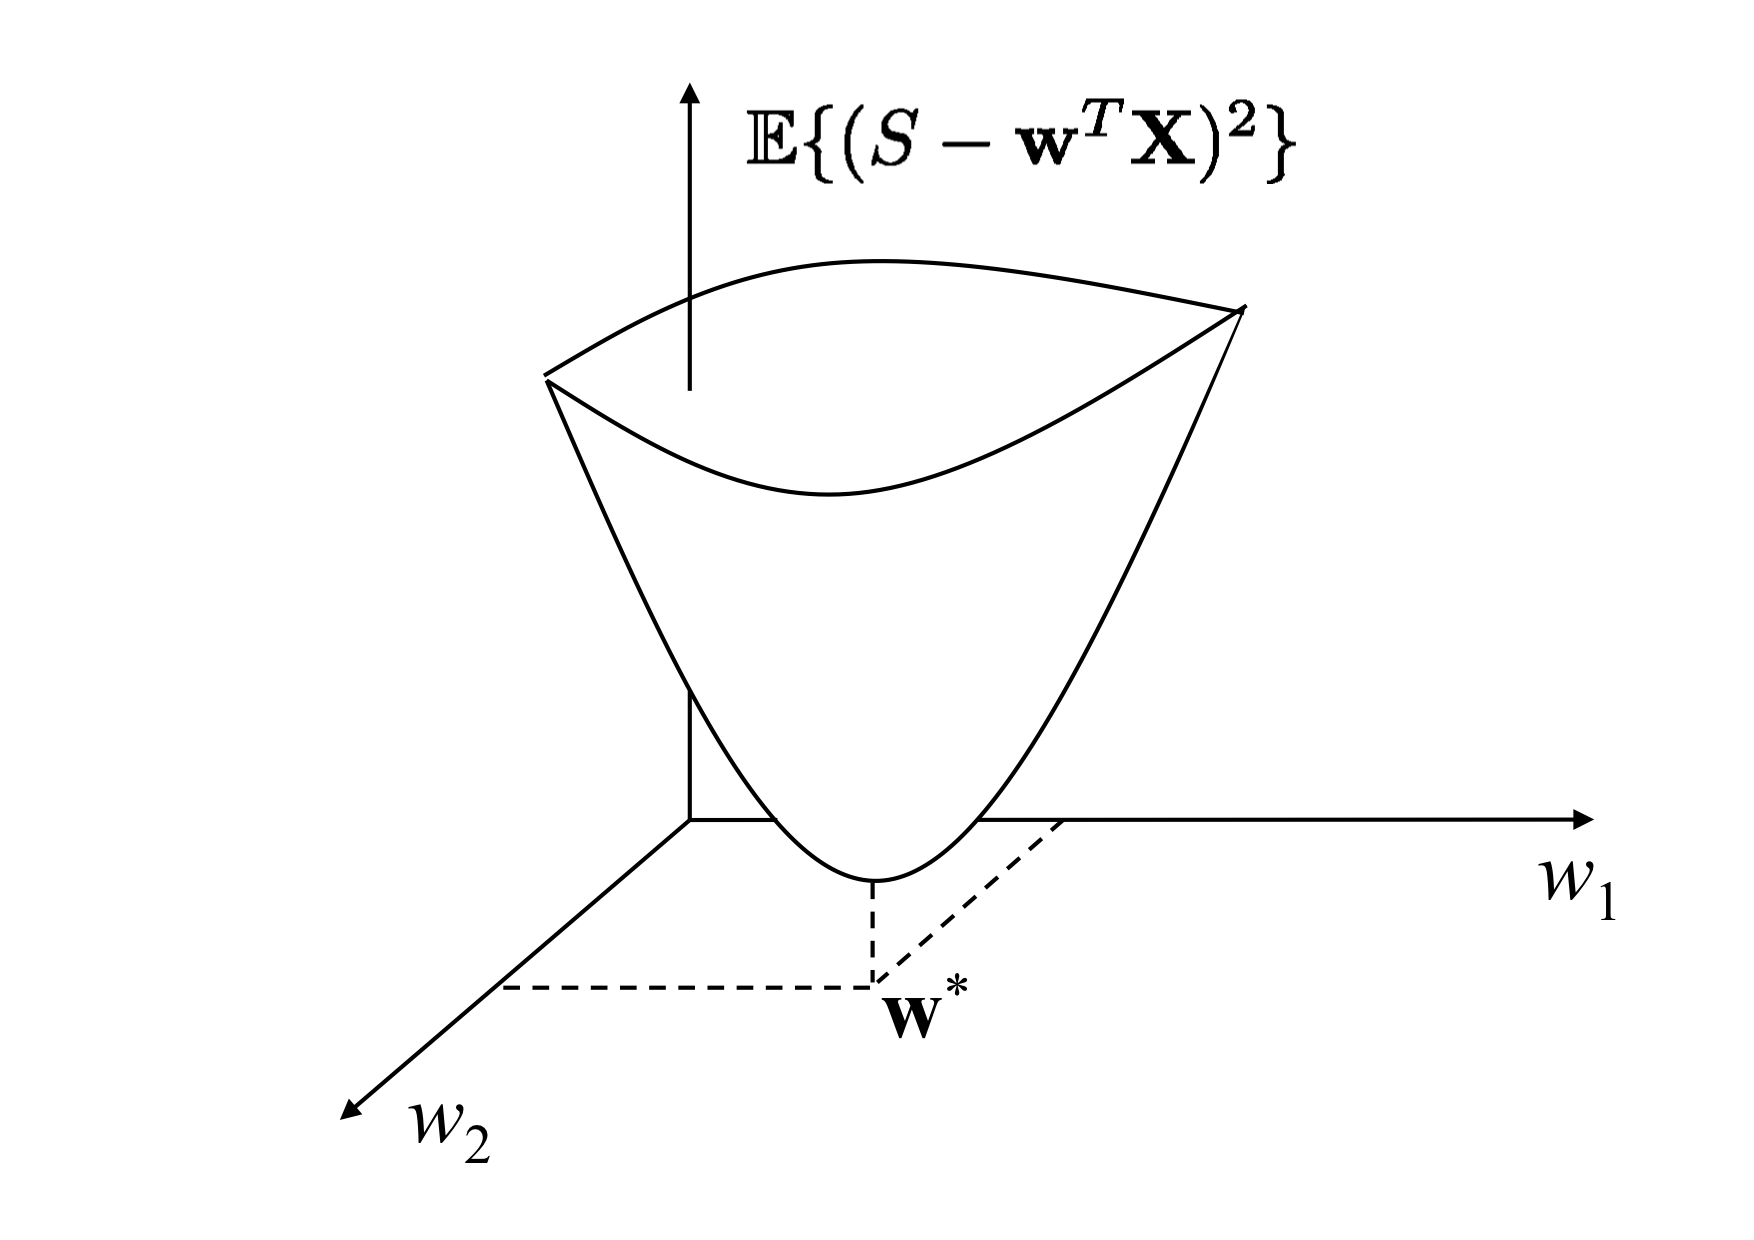
\includegraphics[width=8cm]{Figures//linear_est_error_surface.png}
    \caption{Surface of the MSE for the linear estimator with ${\bf Z}={\bf X}$, as a function of the parameters.}
    \label{fig:linear_est_error_surface}
  \end{center}
\end{figure}
%%%%%%%%%%%%

Since the MSE is non-negative, it is guaranteed to be a convex function of ${\bf w}$ and, thus, its minimum must be located at a point with zero gradient\footnote{The gradient of a function scale $f({\bf w})$ with respect to the vector ${\bf w}$ is defined as a vector formed by the derivatives of the function with respect to each one of the components of $\bf w$: $\nabla_{{\bf w}} f({\bf w}) = \left[\frac{\partial f}{\partial w_1}, \dots \frac{\partial f}{\partial w_N}\right]^T$.} (with respect to ${\bf w}$):
%\begin{align}
%\label{ec:ecs_normales_1}
%\left. \nabla_{\bf w} \EE\{(S - \hat S)^2\} \right|_{{\bf w} = {\bf w}^*} 
% & = \left. -2 \EE\{(S - {\bf w}^T {\bf Z}) {\bf Z}\} \right|_{{\bf w} = {\bf w}^*} = \\
% & = -2 \EE \{(S - {{\bf w}^*}^T {\bf Z}) {\bf Z} \} = {\bf 0}
%\end{align}
{\begin{align}
\label{ec:ecs_normales_1}
\left. \nabla_{\bf w} MSE \right|_{{\bf w} = {\bf w}^*} 
 &= -2 {\bf r}_{S{\bf Z}} + 2 {\bf R}_{\bf Z} {\bf w}^* 
  = {\bf 0}
\end{align}
%The second line of the above expression defines the conditions to be met by the optimal weight vector. Note that this equation is actually a system of $N+1$ equations (as many as dimensions have ${\bf X}_{\text{e}}$) with $N+1$ unknowns (the components of ${\bf w}_{\text{e}^*}$).
%
%In order to find the optimal {weight} vector, it is convenient to rewrite the last line of \eqref{ec:ecs_normales_1} as follows 
%
%\begin{equation}
%\mathbb{E}\{S {\bf X}_{\text{e}} \}
%    = \mathbb{E}\{ {\bf X}_\text{e} ({\bf X}_{\text{e}}^T {\bf w}_{\text{e}}^*)  \}
%\label{Est:EcDelELv}
%\end{equation}
%Defining the cross-correlation vector
%\begin{equation}
%{\bf r}_{S{\bf X}_e} = \mathbb{E}\{S{\bf X}_e\}
%\end{equation}
%and the correlation matrix 
%\begin{equation}
%{{\bf R}_{{\bf X}_e}} = \mathbb{E}\{{\bf X}_e{\bf X}_e^T\}
%\end{equation}
%(which is a symmetric matrix) ec. \eqref{Est:EcDelELv} can be written as
%\begin{equation}
%\label{Est.ec:RxWr}
%{\bf r}_{S{\bf X}_e} = {{\bf R}_{{\bf X}_e}} {\bf w}_{\text{e}}^* 
%\end{equation}
%Thus, the searched weight vector is:
therefore, the optimal weight vector is any solution of
\begin{align}
\label{ec:ecs_normales_2}
{\bf R}_{\bf Z} {\bf w}^* = {\bf r}_{S{\bf Z}}
\end{align}
If the autocorrelation matrix is invertible, we get
\begin{framed}
\begin{equation}
\label{Est.ec:weopt}
 {\bf w}^* = {{\bf R}_{\bf Z}^{-1}} {\bf r}_{S{\bf Z}} 
\end{equation}
\end{framed}}

%
%%%%%%%%%%%%%%%%%%%%%%%%%%%%%%%%%%%%%%%%%%%%%%%%%%%%%%%%
%\subsubsection{Properties of the optimal linear estimator}
%
%Equation \eqref{Est.ec:RxWr} solves the problem of calculating the weights of the estimator $\hat S_\text{LMSE}$. But it is interesting to return to the vector equation  \eqref{ec:ecs_normales_1} to analyze some of its properties. Note that the term in parentheses in this equation is the estimation error
%\begin{equation}
%E^* = S - {{\bf w}_{\text{e}}^*}^T {\bf X}_{\text{e}}
%\end{equation}
%so we can rewrite \eqref{ec:ecs_normales_1} as
%\begin{equation}
%\label{Est:SLMSinsesgado0}
%\mathbb{E}\{E^* {\bf X}_{\text{e}})\} = {\bf 0}
%\end{equation}
%Taking, on the one hand, the first component of this equation (taking into account that $X_{\text{e},1}=1$, and the rest on the other hand, two fundamental properties of the lowest quadratic mean error linear estimator are obtained:
%\begin{description}
%\item[{\bf Property 1:}] The error has zero mean:
%\begin{equation}
%\label{Est:SLMSinsesgado}
%\mathbb{E}\{E^*\} = {\bf 0}
%\end{equation}
%When an estimator has this property it is said that it is {\bf unbiased}.% {Volveremos sobre esta propiedad en la sec. \ref{Est:Sec:CaracterEstim}.}
%\item [{\bf Property 2 (Orthogonality Principle):}] the error is statistically orthogonal to the observations:
%\begin{equation}
%\label{Est:PrincipioOrtV1}
%\mathbb{E}\{E^* {\bf X}\} = {\bf 0}
%\end{equation}
%\end{description}



%%%%%%%%%%%%%%%%%%%%%%%%%%%%%%%%%%%%%%%%%%%%%%%%%%%%%%%%%%%%%%%%%%
\subsubsection{Alternative expression for the linear case}

We can obtain an alternative expression for the optimal weights in the case of the linear estimator with the independent term in \eqref{Est:blin}, \textcolor{blue}{that} can be written as
\begin{align}
\hat S = w_0 + {\bf w}_{1:}^\intercal {\bf X}
\end{align}
where ${\bf w}_{1:}$ is the weight vector after removing the first component, $w_0$. To do so, we can re-express \eqref{ec:ecs_normales_2} as the equivalent pair of equations
\begin{equation}
\label{Est:E0}
\EE\{w_0^* + {{\bf w}_{1:}^*}^\intercal {\bf X} \} = \EE\{S\}
\end{equation}
\begin{equation}
\label{Est:Ex}
\EE\{{\bf X}\} w_0^* + \EE\{{\bf X}{\bf X}^\intercal\}{\bf w}_{1:}^* = \EE\{S{\bf X}\}
\end{equation}
that is
\begin{equation}
w_0^* = m_S - {{\bf w}_{1:}^*}^\intercal{\bf m_x}
\end{equation}
\begin{align}
\label{Est:PrincipioOrtV2b}
\EE\{{\bf X} {\bf X}^\intercal \}{\bf w}_{1:}^* = \EE\{S {\bf X}\} - w_0^* {\bf m_X}  
\end{align}
where $m_S=\EE\{S\}$, $m_{\bf X} =\EE\{{\bf X}\}$. Now using the expressions that relate the correlation and covariance of two variables:
\begin{equation}
\mathbb{E}\{S {\bf X}\} = {\bf v}_{S{\bf X}} + m_S {\bf m_X}
\end{equation}
\begin{equation}
\mathbb{E}\{{\bf X}{\bf X}^\intercal\} = {\bf V_X} + {\bf m_X}{\bf m}_{\bf X}^\intercal
\end{equation}
we get 
\begin{align}
w_0^* &= m_S  - {{\bf w}_{1:}^*}^\intercal{\bf m_x}  \\
\label{Est:PrincipioOrtV2c}
{\bf v}_{S{\bf X}} + m_S {\bf m_X} 
	&= ({\bf V_X} + {\bf m_X}{\bf m}_{\bf X}^T){\bf w}_{1:}^* + w_0^* {\bf m_X}  
\end{align}

{Solving these equations for $w_0^*$ and $w_{1:}^*$ we get
%Expanding Ecs. \eqref{Est:SLMSinsesgado} and \eqref{Est:PrincipioOrtV1}, we can obtain the following explicit formulas for the coefficients $w_0^*$ and ${\bf w}^*$ of the estimator:
\begin{framed}
\begin{equation}
w_0^* = m_S - {{\bf w}_{1:}^*}^T{\bf m_x} 
\label{ec:solucionw0}
\end{equation}
\begin{equation}
\label{ec:solucionw}
{\bf w}_{1:}^* = {{\bf V}_{\bf X}^{-1}} \; {\bf v}_{S,{\bf X}}\end{equation}
\end{framed}}

{The optimal estimator is, thus,
\begin{align}
\label{Est:slmse}
\hat{S}_	\text{LMSE} 
	= m_S + {\bf v}_{S{\bf X}}^\intercal {\bf V}_{\bf X} ({\bf X}-{\bf m}_{\bf X})
\end{align}}

The bias term $w_0$ compensates for differences between the means of the target variable and the observations. Therefore, when all the variables involved have zero mean, $w_0^* = 0$, and the estimator is purely linear in the observations.


% In contrast the weight vector ${\bf w}$ minimizes the mean quadratic error of the fluctuations of $S$ around its mean, exploiting for it the existing statistical relation between $S$ and $\bf X$.

%We will dedicate this section to obtain expressions \eqref{ec:solucionw0} and \eqref{ec:solucionw}. The first is a direct consequence of \eqref{Est:SLMSinsesgado} that can be developed as 
%
%\begin{equation}
%m_S - {{\bf w}^*}^T{\bf m_x} - w_0^* =0 
%\end{equation}
%solving for $w_0^*$, we obtain \eqref{ec:solucionw0}.
%
%{We will now search for an expression for ${\bf w}^*$. From \eqref{Est:PrincipioOrtV1} results
%\begin{equation}
%\label{Est:PrincipioOrtV2}
%\mathbb{E}\{(S - {{{\bf w}^*}^T} {\bf X} - w_0^*) {\bf X}\} = {\bf 0}
%\end{equation}
%which can be rewritten as
%\begin{align}
%\label{Est:PrincipioOrtV2b}
%\mathbb{E}\{S {\bf X}\} 
%   &= \mathbb{E}\{({{\bf w}^*}^T {\bf X} + {w_0^*}) {\bf X}\}     \nonumber\\
%   &= \mathbb{E}\{{\bf X} ({{\bf X}^T{\bf w}^*}) \} {+ w_0^*} \mathbb{E}\{{\bf X} \}  \nonumber\\
%   &= \mathbb{E}\{{\bf X} {\bf X}^T \}{\bf w}^* + w_0^* {\bf m_X}  
%\end{align}
%}
%eq. \eqref{Est:PrincipioOrtV2b} becomes 
%\begin{align}
%\label{Est:PrincipioOrtV3}
%{\bf v}_{S,{\bf X}}  
%   &= {\bf V_X}{\bf w}^* + {\bf m_X}{\bf m}_{\bf X}^T{\bf w}^* + w_0^* {\bf m_X} - m_S {\bf m_X}  \nonumber\\ 
%   &= {\bf V_X}{\bf w}^* 
%    + {\bf m_X}(w_0^* + {\bf m}_{\bf X}^T{\bf w}^* - m_S) 
%     \nonumber\\ 
%   &= {\bf V_X}{\bf w}^* 
%\end{align}
%where, in the last equality, we have applied \eqref{ec:solucionw0}. So, solving for ${\bf w}^*$, we get \eqref{ec:solucionw}.



%%%%%%%%%%%%%%%%%%%%%%%%%%%%%%%%%%%%%%%%%%%%%%%%%%%%%%%%%%%%
\subsubsection{Minimum squared mean error}
 
%Here we will calculate the mean squared error associated with the linear estimator of minimum mean squared error, $\hat S_\text{LMSE}$. As commented at the beginning of this section, the mean squared  error obtained will, in general, be higher than the minimum mean squared error of the Bayesian estimator ($\hat S_\text{MMSE}$), except when this last estimator has precisely a linear structure (in this case, it would be the same).

{The minimum MSE can be computed by replacing the optimal weights \eqref{Est.ec:weopt} into
\eqref{Est:LMSEw}
\begin{align}
\label{Est:LMSEw2}
\text{MSE}^* &= \EE\{S^2\} 
     - 2 {\bf r}_{S{\bf Z}}^\intercal {{\bf R}_{\bf Z}^{-1}} {\bf r}_{S{\bf Z}}  
     + ({{\bf R}_{\bf Z}^{-1}} {\bf r}_{S{\bf Z}} )^\intercal {\bf R}_{\bf Z} 
       {{\bf R}_{\bf Z}^{-1}} {\bf r}_{S{\bf Z}}    \nonumber\\
    &= \EE\{S^2\} 
     - {\bf r}_{S{\bf Z}}^\intercal {{\bf R}_{\bf Z}^{-1}} {\bf r}_{S{\bf Z}}  
\end{align}}

For the linear estimator \eqref{Est:slmse}
%in mean squared error we only have to develop the expression of the MSE, particularizing for $\hat S_\text{LMSE}$ and leaving the result in function of the mathematical expectations of the involved random variables:
%\begin{align}
%\mathbb{E}\{(S - \hat S_\text{LMSE})^2\} 
%   & = \mathbb{E}\{E^*(S - w_0^* - {{\bf w}^*}^T {\bf X})\} \nonumber\\ 
%   & = \mathbb{E}\{E^* S\} 
%     - w_0^* \mathbb{E}\{E^*\} 
%     - {{\bf w}^*}^T \mathbb{E}\{{\bf X}E^*\}  \nonumber\\
%   & = \mathbb{E}\{E^* S\} 
%\end{align}
%where, in the last equality, we have applied the two properties of the minimum quadratic mean error estimator obtained in \eqref{Est:SLMSinsesgado} and \eqref{Est:PrincipioOrtV1}. Operating again the error term, $E^*$, results in
%\begin{align}
%\mathbb{E}\{(S - \hat S_\text{LMSE})^2\} 
%   & = \mathbb{E}\{S (S - w_0^* - {{\bf w}^*}^T {\bf X})\}  \nonumber\\
%   & = \mathbb{E}\{S^2\} 
%     - w_0^* m_S 
%     - {{\bf w}^*}^T ({\bf v}_{S{\bf X}} + m_S {\bf m}_{\bf X})\} \nonumber\\
%   & = \mathbb{E}\{S^2\} - m_S (w_0^* {+} {{\bf w}^*}^T {\bf m}_{\bf X})
%     - {{\bf w}^*}^T {\bf v}_{S{\bf X}}  \nonumber\\
%   & = v_S - {{\bf w}^*}^T {\bf v}_{S{\bf X}} 
%\end{align}
\begin{align}
\text{MSE}^* = v_S - {{\bf w}^*}^T {\bf v}_{S{\bf X}} 
\end{align}

%\begin{exercise}[Cálculo del error cuadrático medio para variables con medias nulas]
%Demuestre el resultado \eqref{ec:err_LMSE} para el caso concreto en que $\mathbb{E}\{S\} = 0$ y $\mathbb{E}\{{\bf X}\} = {\bf 0}.$
%\end{exercise}

%%%%%%%%%%%%%%%%%%%%%%%%%%%%%%%%%%%%%%
\section{Estimation with Gaussian distributions}
%%%%%%%%%%%%%%%%%%%%%%%%%%%%%%%%%%%%%%

In this section, we delve into the estimation of random variables within the context where the combined distribution of all involved variables (the target variable along with the observational variables) is a multidimensional Gaussian. This scenario is particularly significant due to the prevalent occurrence of these distributions in signal processing, communications and various other fields. 

When the joint distribution $p_{S,{\bf X}} (s, {\bf x})$ is Gaussian, all marginal and conditional distributions retain a Gaussian form. In particular, the posterior distribution, $p_{S|{\bf X}} (s|{\bf x})$ is Gaussian. Since the mean, median, and mode of the Gaussian distribution align, $\sMSE = \sMAD = \sMAP$. Thus, our discussion in this section will primarily concentrate on deriving the estimator that minimizes the MSE.

Besides, we will demonstrate that the minimum MSE estimator and, consequently, the MAP and MAD estimators are linear, which will allow us to use the results shown in the previous section for minimum MSE estimation.


%%%%%%%%%%%%%%%%%%%%%%%%%%%%%%%%%%%%%%
\subsection{One dimensional variables}

\textcolor{blue}{Assume that the joint} distribution of $X$ and $S$ is Gaussian:
\begin{equation}
p_{S,X}(s,x) \sim G\left(\begin{bmatrix} s \\ x \end{bmatrix},
                         \begin{bmatrix} v_X & \rho \\ \rho & v_S \end{bmatrix}\right)
\end{equation}
where $\rho$ is the covariance between the two random variables. From the joint distribution, we can obtain any other distribution involving the variables $S$ and $X$; specifically, the posterior distribution can be obtained as:
\begin{align}
\label{Est_psxgauss}
p_{S|X}(s|x) 
	&= \frac{p_{S,X}(s,x)}{p_X(x)} 
	 = \frac{\frac{1}{2\pi \sqrt{v_X v_S - \rho^2}}
	         \exp\left[-\dfrac{1}{2(v_X v_S - \rho^2)} 
	         			\begin{bmatrix} s \\ x \end{bmatrix}^\intercal
	                    \begin{bmatrix} v_X & -\rho \\ -\rho & v_S \end{bmatrix} 
	                    \begin{bmatrix} s \\ x \end{bmatrix}\right]}
	        {\frac{1}{\sqrt{2\pi v_X}} \exp\left[-\frac{x^2}{2 v_X}\right]}
\end{align}
where it has been necessary to calculate the inverse of the covariance matrix of $S$ and $X$. 

{Noting that, as a function of $s$, $p_{S|X}(s|x)$ differs from $p_{S,X}(s,x)$ in the scale factor $p_X(x)$, which does not depend on $s$,  $p_{S|X}(s|x)$ should be a Gaussian pdf too. Therefore, it must be writable as
\begin{align}
\label{Est_postsxgauss}
p_{S|X}(s|x) = \frac{1}{\sqrt{2\pi v_{S|X}}} \exp\left[ -\frac{(s - m_{S|X})^2}{2 v_{S|X}}\right] 
\end{align}
where $m_{S|X}$ and $v_{S|X}$ are the posterior mean and variance, respectively, to be determined.}

Joining \eqref{Est_psxgauss} and \eqref{Est_postsxgauss}, we can write
\begin{align}
\frac{2\pi \sqrt{v_X v_S - \rho^2}}{\sqrt{2\pi v_{S|X}}\sqrt{2\pi v_X}} 
\exp\left[- \frac{(s - m_{S|X})^2}{2 v_{S|X}}
          + \frac{1}{2(v_X v_S - \rho^2)} \begin{bmatrix} s \\ x \end{bmatrix}^T
	                                      \begin{bmatrix} v_X & -\rho \\ -\rho & v_S \end{bmatrix} 
	                                      \begin{bmatrix} s \\ x \end{bmatrix}    
	      - \frac{x^2}{2 v_X}
	\right] = 1
\end{align}
{which can be simplified to
\begin{align}
\frac{\sqrt{v_X v_S - \rho^2}}{\sqrt{v_{S|X} v_X}} 
\exp\left[- \frac{s^2 - 2m_{S|X} s + m_{S|X}^2}{2 v_{S|X}}
          + \frac{v_X s^2 - 2 \rho x s + v_S x^2}{2(v_X v_S - \rho^2)}     
	      - \frac{x^2}{2 v_X}
	\right] = 1
\end{align}
Note that the equation above must be satisfied for any $s\in\mathbb{R}$. Since the right-hand side is constant, and the exponent on the left-hand side is a polynomial function of $s$, the coefficients multiplying $s^2$  and $s$ must be zero. Thus}
\begin{equation}
\label{ec:gauss_iguald4}
\frac{m_{S|X}}{v_{S|X}} = \frac{\rho x}{v_X v_S - \rho^2}
\end{equation}
\begin{equation}
\label{ec:gauss_iguald5}
\frac{1}{v_{S|X}} = \frac{v_X}{v_X v_S - \rho^2}
\end{equation}
{From \eqref{ec:gauss_iguald5} we get the posterior variance
\begin{framed}
\begin{equation}
\label{Est_posterior_var_gauss}
v_{S|X} = v_S - \frac{\rho^2}{v_X}
\end{equation}
\end{framed}
\noindent and, replacing \eqref{Est_posterior_var_gauss} into \eqref{ec:gauss_iguald4} we get the posterior mean, which is the minimum MSE estimate}
\begin{framed}
\begin{equation}
\label{ec_estimador_caso_gaussiano_final}
\sMSE = \sMAD = \sMAP = m_{S|X} = \frac{\rho}{v_X} x
\end{equation}
\end{framed}
Note that the estimator is a \underline{linear} function of the observation.

%%%%%%%%%%%%%%%%
\begin{exercise}
Generalize the above result for the case where the variables $S$ and $X$ have (non-zero) means $m_S$ and $m_X$, respectively. Demonstrate that in such a case, the estimator is
\begin{equation}
\hat s_{\text{MSE}} = m_S + \frac{\rho}{v_X} (x - m_X)
\end{equation}
\end{exercise}
%%%%%%%%%%%%%%

%%%%%%%%%%%%%%%
\begin{example}[Estimation of a Gaussian signal contaminated by Gaussian noise]
\label{ex:senialenruido}

In this example, we will consider the case in which the observation is the sum of the target variable and an independent noise component: $X = S + R$. Both the target and the noise are zero-mean Gaussian random variables with variances $v_S$ and $v_R$, respectively.

Figure \eqref{fig:estimacion_caso_gauss} represents the situation described for a case with $v_S < v_R$.
%\centering
%\begin{tabular}{cc}
%\includegraphics[width=6cm]{Figures/px_s_funcionx.png} &
%\includegraphics[width=6cm]{Figures/px_s_funcions.png}\\
%   (a) & (b)
%\end{tabular}
%\captionof{figure}{Representation of the likelihood distribution of the example %\ref{ex:est_ML_varaleat} as a function of $x$ and $s$.}
%\label{fig:est_ML_caso1}

\begin{center}
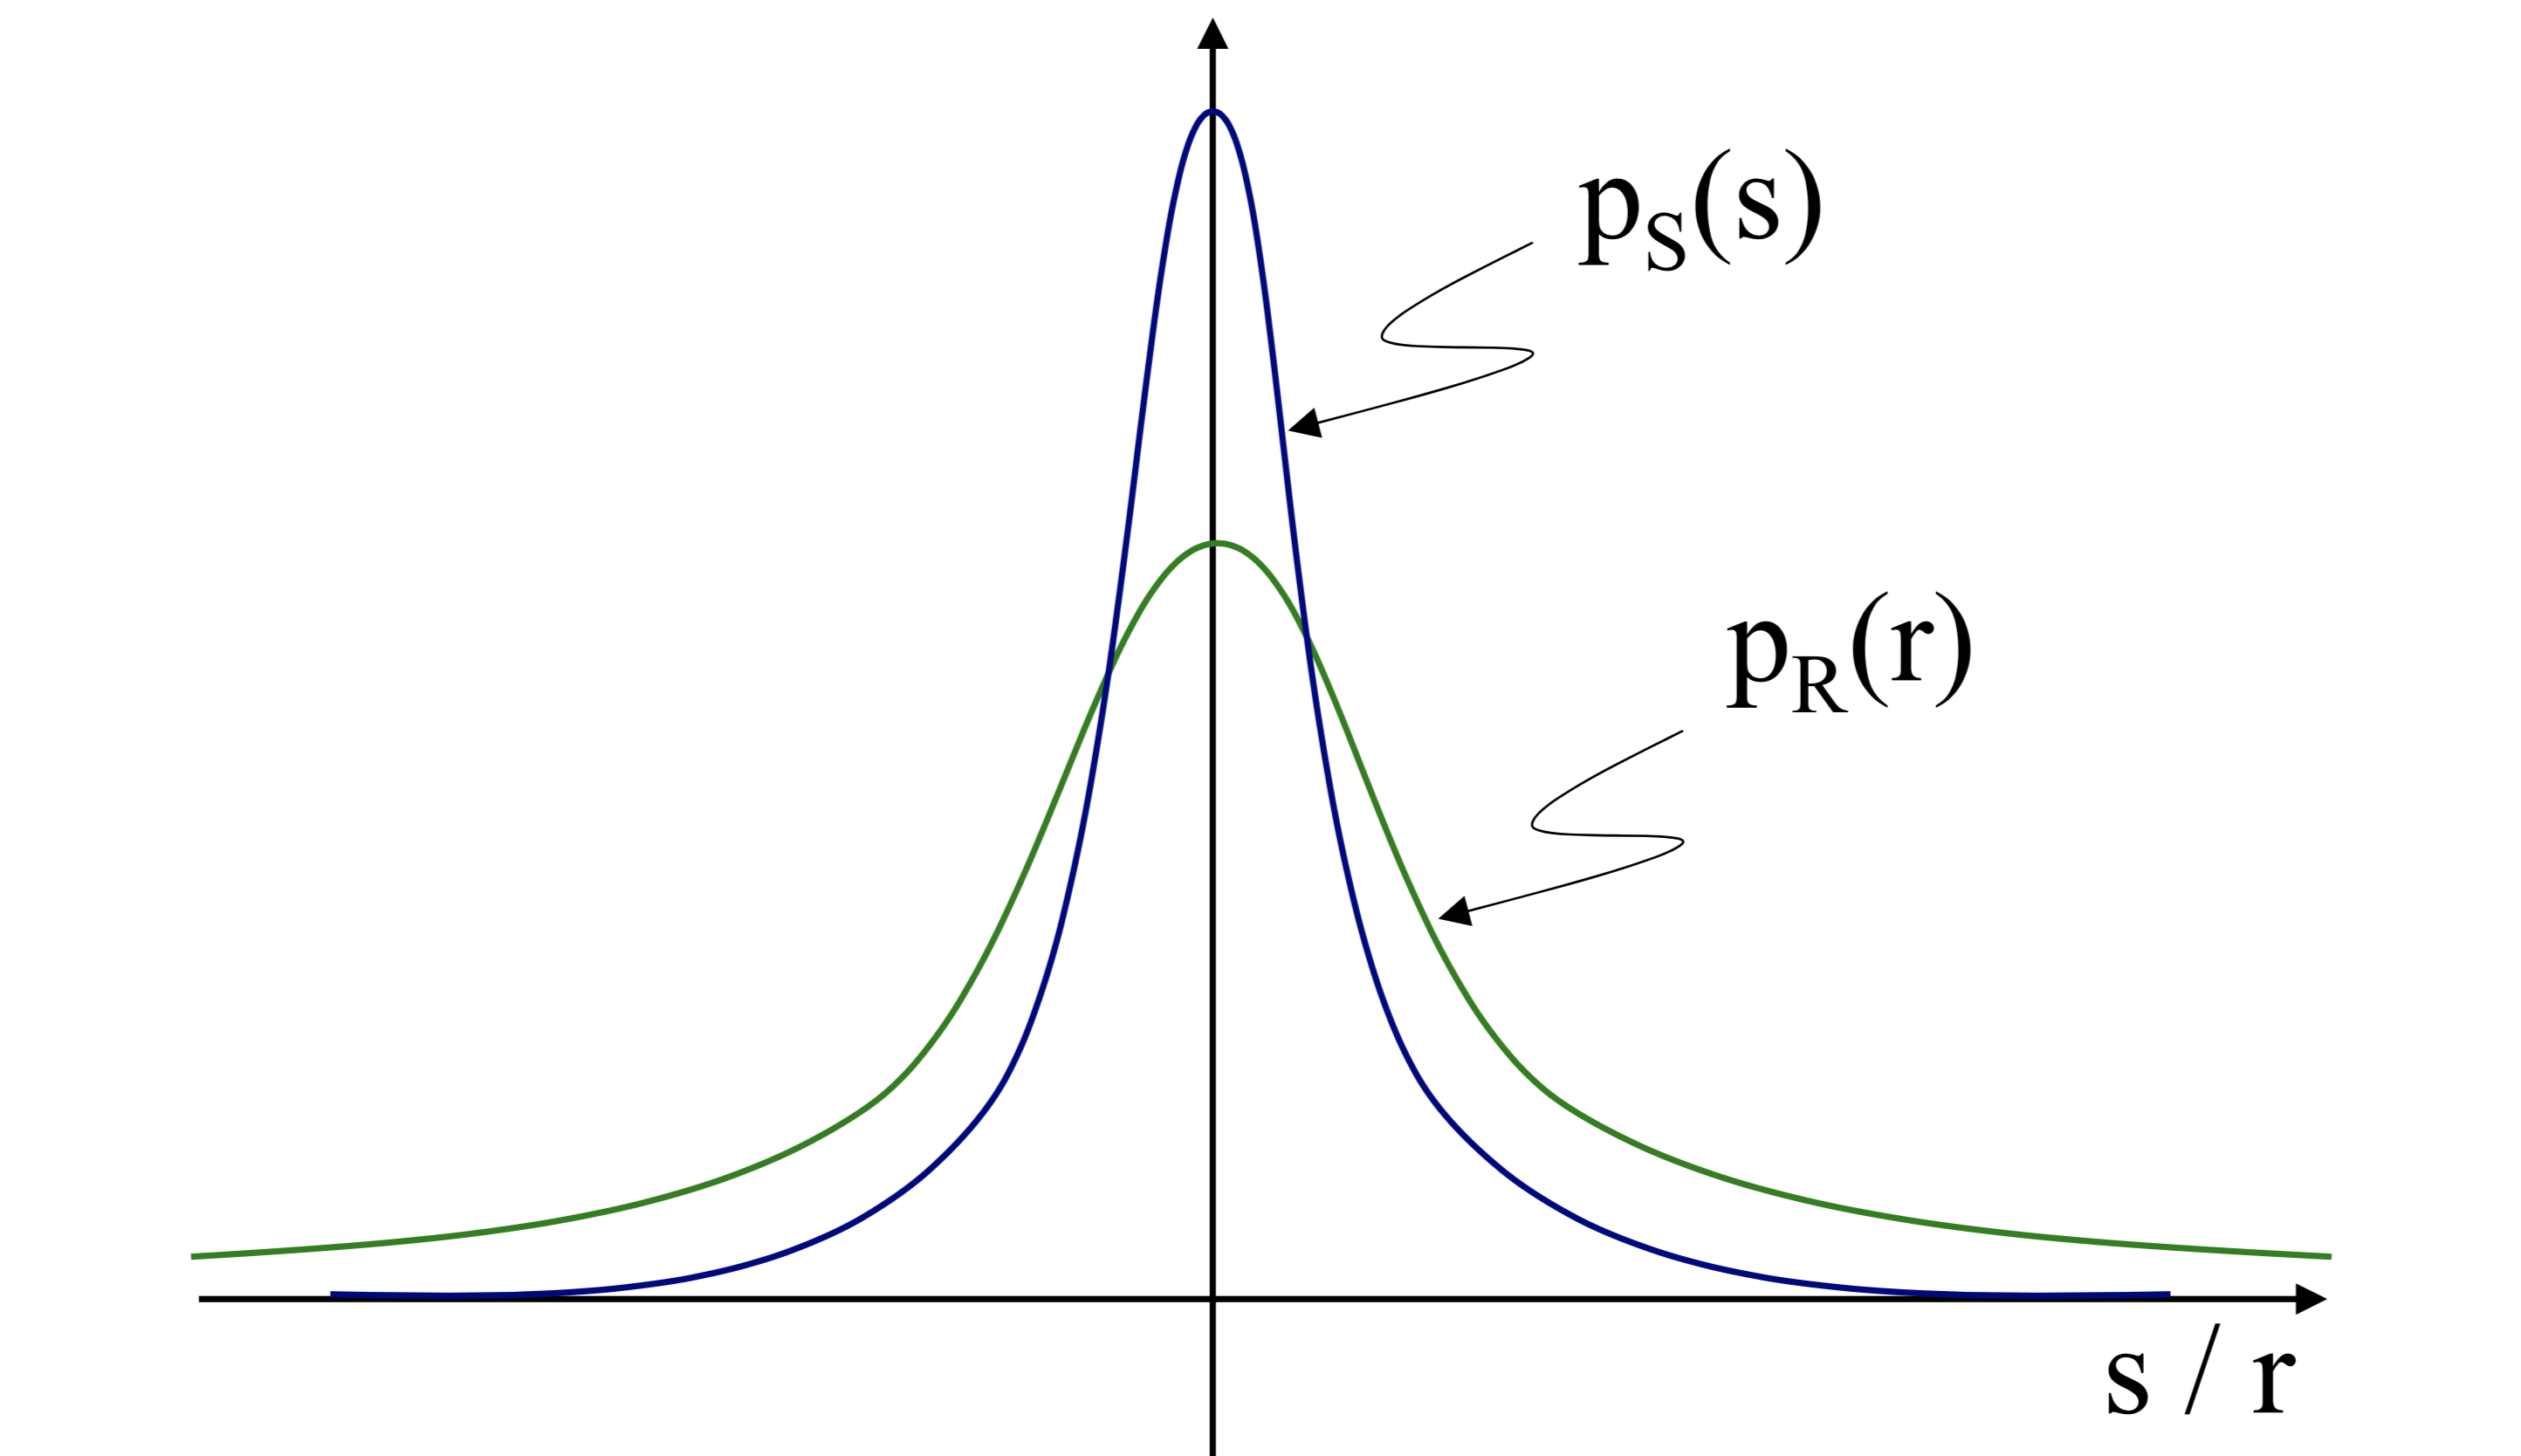
\includegraphics[width=7cm]{Figures//estimacion_caso_gauss.png}
\captionof{figure}{Estimation of Gaussian random variable $S$ contaminated by Gaussian noise $R$.}
\label{fig:estimacion_caso_gauss}
\end{center}

% \begin{figure}[htb]
%  \begin{center}
%  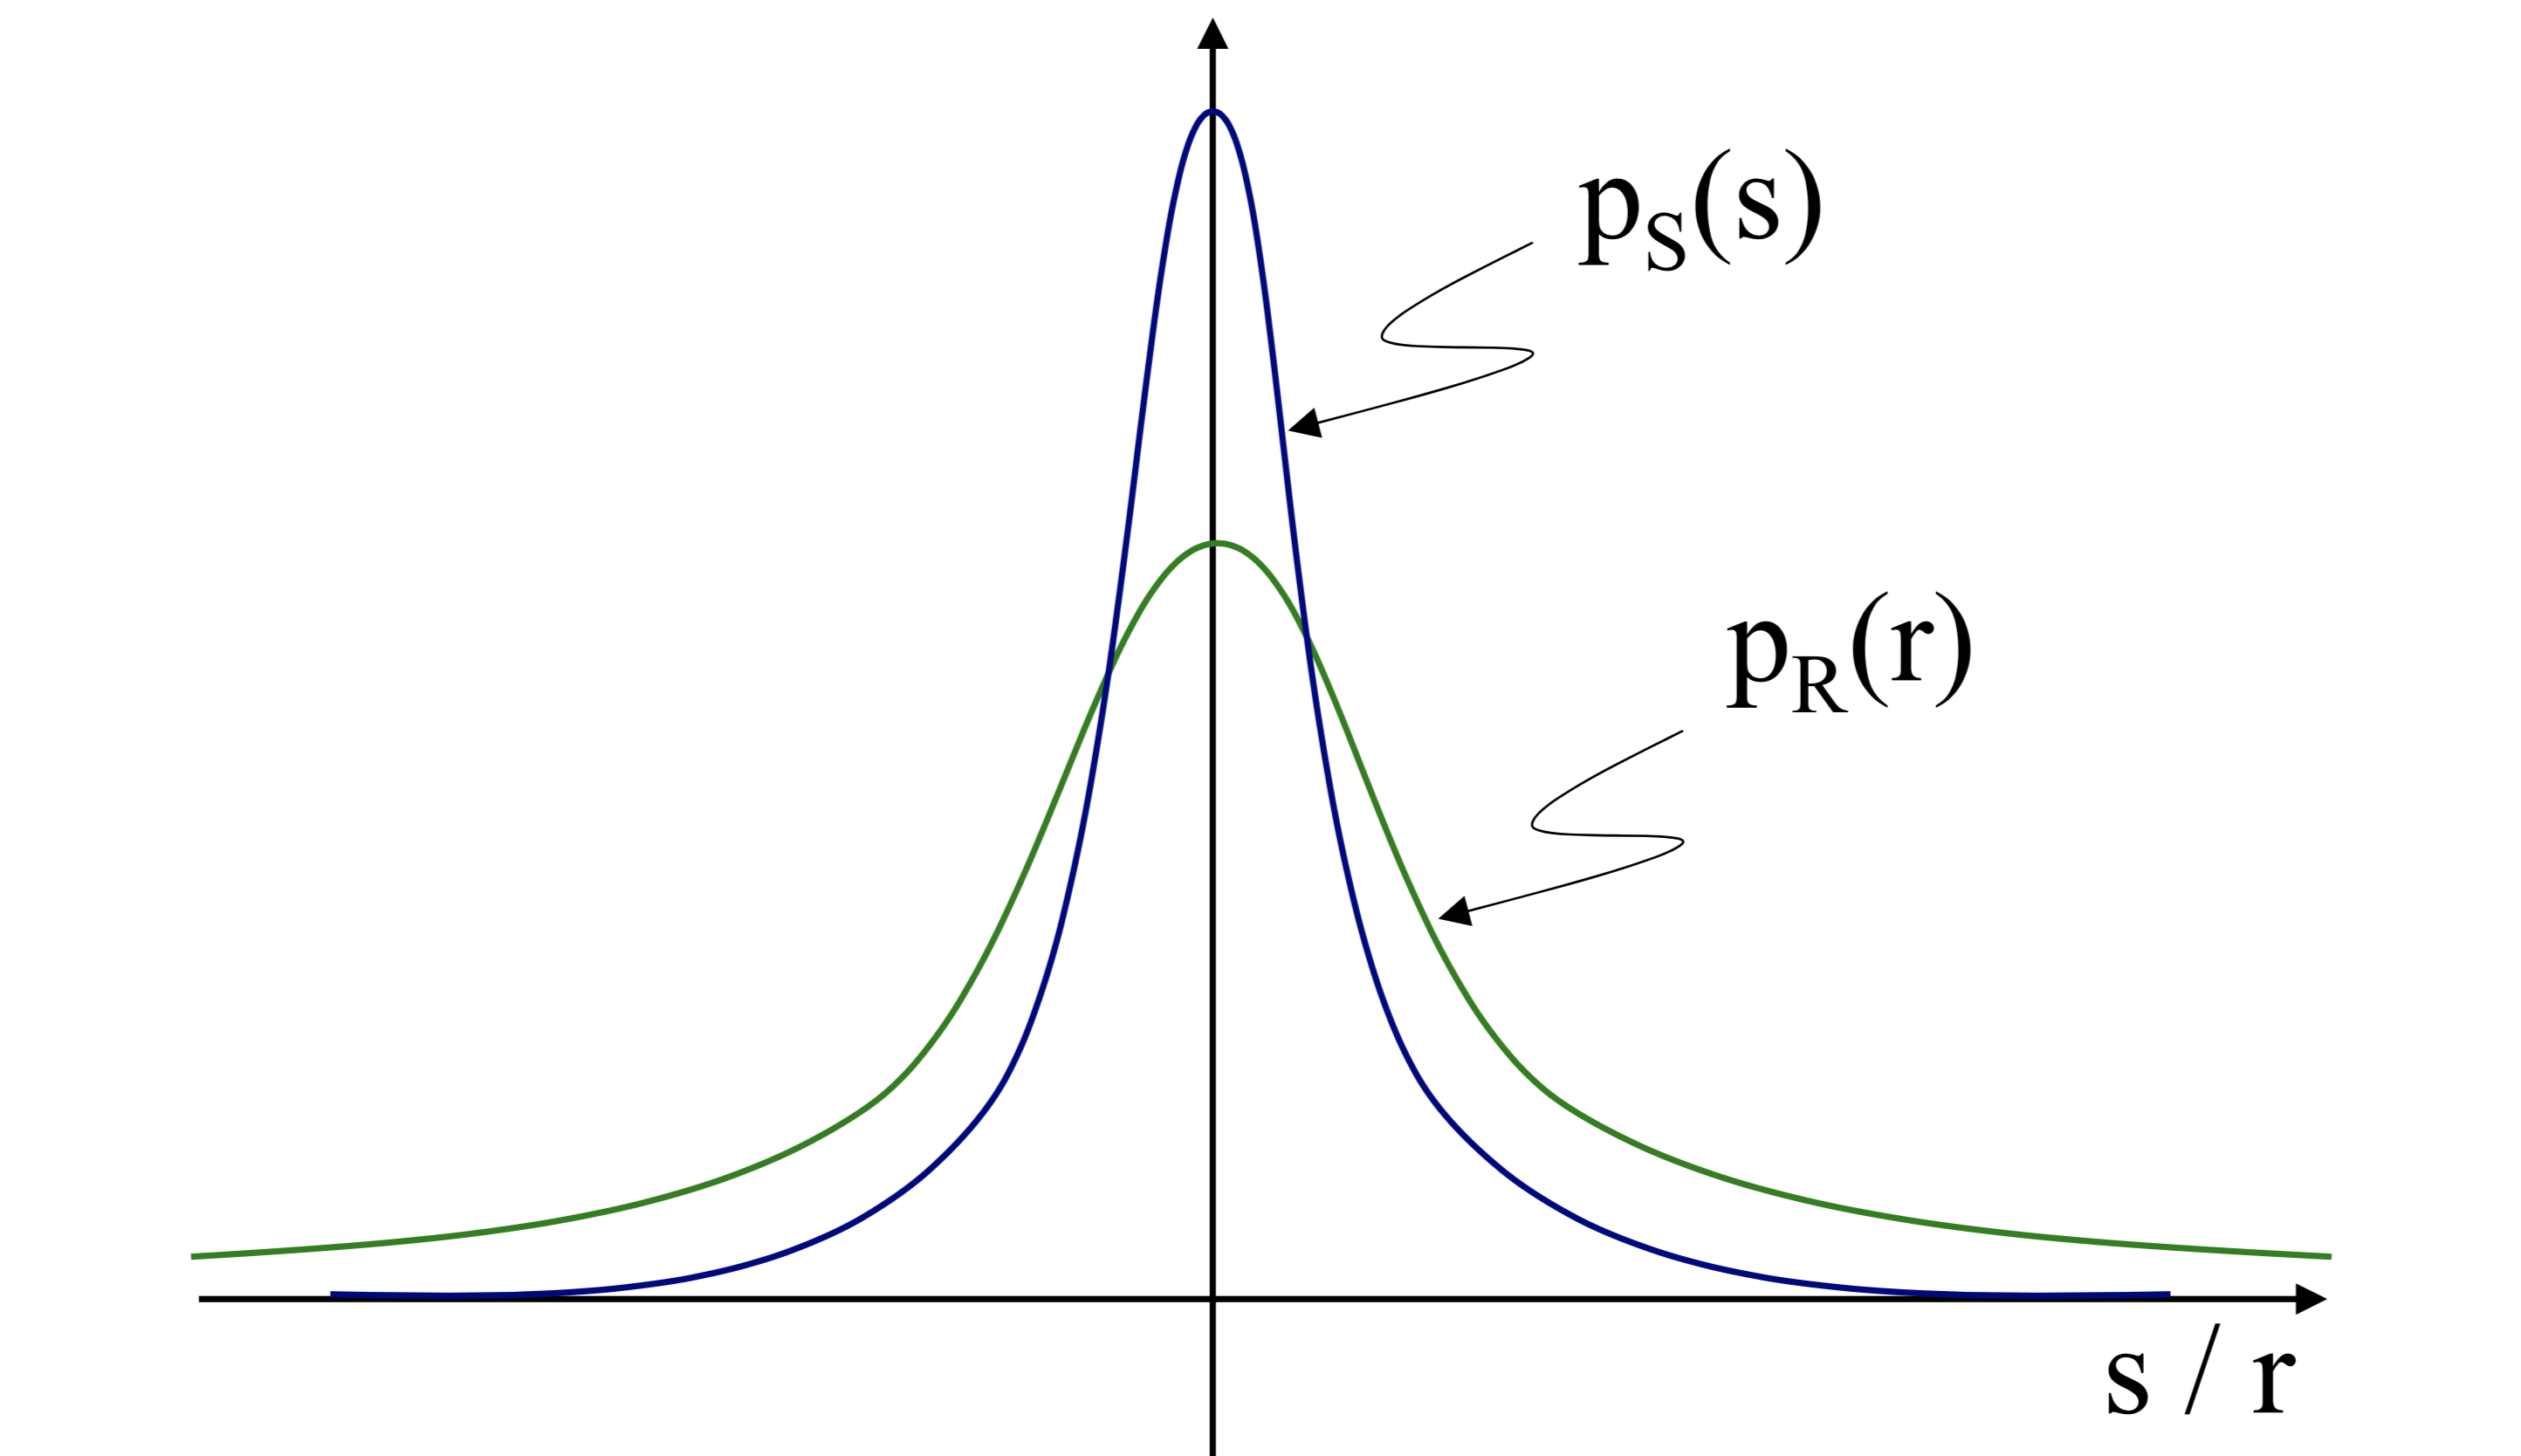
\includegraphics[width=7cm]{Figures//estimacion_caso_gauss.png}
%    \caption{Estimation of Gaussian random variable $S$ contaminated by Gaussian noise $R$.}
%    \label{fig:estimacion_caso_gauss}
%  \end{center}
% \end{figure}

According to \eqref{ec_estimador_caso_gaussiano_final}, for the resolution of the problem, we must find the variance of $X$ and the covariance between $S$ and $X$ ($\rho$). The variance $v_X$ is obtained simply as the sum of $v_S$ and $v_R$ because both are independent variables. For the covariance calculation,
\begin{equation}
\rho = \mathbb{E} \{(X-m_X)(S-m_S)\} = \mathbb{E} \{X\;S\} = \mathbb{E} \{(S + R) S\} = \mathbb{E} \{S^2\} + \mathbb{E} \{S\;R\} = v_S
\end{equation}
where independence of $S$ and $R$ has been used, and the fact that all variables (including $X$) have zero means.

Replacing these results in \eqref{ec_estimador_caso_gaussiano_final} we get
\begin{equation}
\hat s_{\text{MSE}} = \frac{v_S}{v_S + v_R} x
\end{equation}

This result can be interpreted quite intuitively: when the variance of the noise is much lower than that of the signal (high Signal to Noise Ratio (SNR), $v_S \gg v_R$) we get $\hat s_{\text{MSE}} \to x$, which makes sense since the effect of the noise component, in this case, is not very significant; on the contrary, when the SNR is very small ($v_S \ll v_R$), the observation barely provides information about the $S$ value in each experiment, so the estimator keeps the mean value of the signal component, $\sMSE \to 0$.
\end{example} %\vspace{0.4cm}
%%%%%%%%%%%%%


%%%%%%%%%%%%%%%%%%%%%%%%%%%%%%%%%%%%%%%
\subsection{Multidimensional variables}

{In a general multidimensional case, ${\bf S}$ and ${\bf X}$ can be random vectors of dimensions $N$ and $M$, respectively, with joint Gaussian distribution.
\begin{equation}
p_{{\bf S},{\bf X}}({\bf s},{\bf x}) 
   \sim G\left(\left[\begin{array}{c} {\bf m_S} \\ {\bf m_X} \end{array}\right],
               \left[\begin{array}{cc} {\bf V_S}          & {\bf V_{SX}}   \\ 
                                       {\bf V}_{\bf SX}^T & {\bf V_{X}}   
                     \end{array}\right]\right)
\end{equation}
being ${\bf m_S}$ and ${\bf m_X}$ the means of $ {\bf S}$ and $ {\bf X}$, respectively, ${\bf V_S}$ and ${\bf V_X}$ the covariance matrix of ${\bf S}$ and  ${\bf X}$, respectively, and ${\bf V_{SX}}$ the matrix of crossed covariances of ${\bf S}$ and ${\bf X}$, that is,
\begin{align}
{\bf V_S} &= \mathbb{E}\{({\bf S}-{\bf m_S})({\bf S}-{\bf m_S})^\intercal\} \\
{\bf V_X} &= \mathbb{E}\{({\bf X}-{\bf m_X})({\bf X}-{\bf m_X})^\intercal\} \\
{\bf V_{SX}} &= \mathbb{E}\{({\bf S}-{\bf m_S})({\bf X}-{\bf m_X})^\intercal\}
\end{align}
%La expresión general de la densidad de probabilidad es, por tanto
%\begin{align}
%p_{{\bf S},{\bf X}}({\bf s},{\bf x}) 
%   & = \frac{1}
%            {(2\pi)^{(M+N)/2} 
%             \left|\left[\begin{array}{cc} 
%                          {\bf V_S}    & {\bf V_{SX}}   \\ 
%                          {\bf V}_{\bf SX}^T & {\bf V_{X}} 
%                         \end{array}\right]
%             \right|^{1/2}} \times \nonumber\\
%    &  \times\exp\left[-\frac{1}{2}
%                  \left[\begin{array}{c} {\bf s}-{\bf m_S} \\ {\bf x}-{\bf m_X} \end{array}\right]^T                       
%                  \left[\begin{array}{cc} 
%                           {\bf V_S}          & {\bf V_{SX}} \\ 
%                           {\bf V}_{\bf SX}^T & {\bf V_{X}} 
%                        \end{array}\right]^{-1}
%                  \left[\begin{array}{c} {\bf s} \\ {\bf x} \end{array}\right]
%       \right]
%\end{align}
%La distribución a posteriori de $S$ se puede obtener como:
%\begin{align}
%p_{{\bf S}|{\bf X}}({\bf s}|{\bf x}) 
%   & = \frac{p_{{\bf S},{\bf X}}(s,x)}{p_{\bf X}(x)} \nonumber\\
%   & = \frac{(2\pi)^{M/2}|{\bf V}_{\bf X}|^{1/2}}
%            {(2\pi)^{(M+N)/2} 
%             \left| \left[\begin{array}{cc} 
%                             {\bf V_S}    & {\bf V_{SX}}   \\ 
%                           {\bf V}_{\bf SX}^T & {\bf V_{X}} 
%                    \end{array}\right]
%                    \right|^{1/2}} \times \nonumber\\
%    &  \times\exp\left[-\frac{1}{2}
%                  \left[\begin{array}{c} {\bf s} \\ {\bf x} \end{array}\right]^T                       
%                  \left[\begin{array}{cc} 
%                           {\bf V_S}          & {\bf V_{SX}} \\ 
%                           {\bf V}_{\bf SX}^T & {\bf V_{X}} 
%                        \end{array}\right]^{-1}
%                  \left[\begin{array}{c} {\bf s} \\ {\bf x} \end{array}\right]
%                 -\frac{1}{2} {\bf x}^T{\bf V_X}^{-1}{\bf x} \right]
%\end{align}

The calculation of the posterior distribution of ${\bf S}$ given ${\bf X}$ is more complex than in the one-dimensional case, but it follows a similar procedure, which we will omit here. It can be shown that the posterior distribution is Gaussian with mean
\begin{align}
{\bf m}_{{\bf S}|{\bf X}} 
      = {\bf m}_{\bf S} + {\bf V}_{\bf SX}{\bf V_X}^{-1}({\bf x}-{\bf m}_{\bf X}) 
\label{Est:sMMSEgaussMN}
\end{align}
and covariance
\begin{align}
{\bf V}_{{\bf S}|{\bf X}} 
      = {\bf V_S}- {\bf V}_{\bf SX}{\bf V_X}^{-1}{\bf V}_{\bf SX}^T
\end{align}
Since the minimum MSE estimator of ${\bf S}$ given ${\bf X}$ is precisely the posterior mean, we can write
\begin{framed}
\begin{align}
\hat{\bf s}_{\text{MSE}} = \hat{\bf s}_{\text{MAD}} = \hat{\bf s}_{\text{MAP}} = 
{\bf m}_{{\bf S}|{\bf X}} = {\bf m}_{\bf S} + {\bf V}_{\bf SX}{\bf V_X}^{-1}({\bf x}-{\bf m}_{\bf X}) 
\label{Est:sMMSEgaussGral}
\end{align}
\end{framed}
%This estimator expression is simplified when ${\bf S}$ and ${\bf X}$ have zero means, resulting in
%\begin{align}
%\hat{\bf s}_{\text{MSE}} = {\bf m}_{{\bf S}|{\bf X}} 
%      = {\bf V}_{\bf SX}{\bf V_X}^{-1}{\bf x} 
%      \label{Est:sMMSEgaussMN0}
%\end{align}}
%Partiendo de \eqref{Est:sMMSEgaussMN0} pueden obtenerse diversos casos particulares de interés en aplicaciones prácticas del procesado de señales. Algunos de ellos se analizan en el Apéndice \ref{Sec:Est:CasosGauss}.

%%%%%%%%%%%%%%%%%%%%%%%%%%%%%%%%%%%%%%%%%%%%%%%%%%%%%%
\subsection{Linear estimation and Gaussian estimation}

{Note that, if the target variable is scalar, \eqref{Est:sMMSEgaussGral} is identical to \eqref{Est:slmse}. This is not coincidental: if the minimum MSE estimator in the Gaussian case is linear, it must be equal to the best linear estimator, which is given by \eqref{Est:sMMSEgaussGral}.}

%Regrouping the terms of \eqref{Est:sMMSEgaussGral}, we can express $\hat{\bf s}_{\text{MSE}}$ as:
%\begin{framed}
%\begin{align}
%\hat{\bf s}_{\text{MSE}} = ({\bf m}_{\bf S} - {\bf V}_{\bf SX}{\bf V_X}^{-1}{\bf m}_{\bf X} )+ {\bf V}_{\bf SX}{\bf V_X}^{-1}{\bf x} 
%\end{align}
%\end{framed}
%and identifying these terms with the coefficients of a linear estimator, we get
%\begin{align} 
%{\bf w}^T =  {\bf V}_{\bf SX}{\bf V_X}^{-1}
%\end{align}
%\begin{align} 
%w_0 = {\bf m}_{\bf S} - {\bf w}^T {\bf m}_{\bf X}
%\end{align}
%These expressions align with the alternative solution of the linear estimation of mean squared error (equations \ref{ec:solucionw0} and  \ref{ec:solucionw}). This is not surprising: since the unrestricted MSE estimator in the Gaussian case is linear, the best linear estimator must match the one obtained for the Gaussian case.

%Obsérvese, por último, que \eqref{ec:solucionw} asume que {${\bf V}_{\bf X}$} es una matriz no singular. La invertibilidad de {${\bf V}_{\bf X}$} implica que ninguna componente de ${\bf X}$ puede obtenerse como combinación lineal del resto de componentes. Cuando esto no es así, puede comprobarse que la solución al problema de minimización no es única, y por lo tanto conviene eliminar las variables redundantes antes de proceder al diseño del estimador.


%%%%%%%%%%%%%%%%%%%%%%%%%%%%%%%%%%%%%%
\section{ML estimation of probability distributions parameters}
%%%%%%%%%%%%%%%%%%%%%%%%%%%%%%%%%%%%%%

Sometimes we may be interested in estimating the parameters of a probability distribution, such as the mean or variance of a Gaussian distribution, the decay parameter that characterizes an exponential distribution, or values $a$ and $b$ delimiting the interval in which a uniform distribution is defined.

In these cases, the prior distribution of these variables is not usually known, even more, in many cases, these parameters are said to be deterministic and are not treated as random parameters. However, if a set of observations generated from these distributions is available, we can obtain the likelihood of these variables and estimate their values with maximum likelihood criteria.

% Note that in order to use some Bayesian estimator, it would be necessary to know the posterior and without having information on the prior of these parameters we cannot know the posterior. Therefore, the only estimator we can apply in this scenario is the maximum likelihood estimator.

%%%%%%%%%%%%%%%
\begin{example}[ML estimate of the mean and variance of a one-dimensional Gaussian distribution]
\label{ex:gauss_ML}

The weight of individuals in a family of molluscs is known to obey a Gaussian distribution, but the mean and variance are unknown. The weight of $l$ individuals taken independently, $\{X^{(k)}\}_{k=1}^l$, is available.

The likelihood of the mean and the variance for a single observation $x$, in this case, is given by:
\begin{equation}
p_{X}(x) = p_{X|m,v}(x|m,v) = \frac{1}{\sqrt{2\pi v}} \exp\left[-\frac{(x-m)^2}{2 v}\right]
\end{equation}
Since we must construct the estimator based on the joint observation of $l$ observations, we will need to calculate the joint distribution of all of them which, being independent observations, is obtained as the product of individual observations:
\begin{equation}
\label{ec:conjunta_est_ML_gauss}
\begin{split}
p_{\{X^{(k)}\}|m,v}(\{x^{(k)}\}|m,v) 
	& = \prod_{k=1}^l p_{X|m,v}(x^{(k)}|m,v) \\ 
		&= \frac{1}{(2\pi v)^{l/2}} \prod_{k=1}^l \exp\left[-\frac{(x^{(k)}-m)^2}{2 v}\right]
\end{split}
\end{equation}
The ML estimators of $m$ and $v$ will be the values maximizing \eqref{ec:conjunta_est_ML_gauss}. The analytical form of this function suggests the use of the logarithm to simplify the maximization:
\begin{equation}
\label{ec:conjunta_est_ML_gauss_log}
L = \ln \left[ p_{\{X^{(k)}\}|m,v}(\{x^{(k)}\}|m,v) \right] = -\frac{l}{2} \ln(2\pi v) - \frac{1}{2v} \sum_{k=1}^l (x^{(k)}-m)^2
\end{equation}

Differentiating \eqref{ec:conjunta_est_ML_gauss_log} with respect to $m$ and $v$, we get the system of equations to solve
\begin{equation}
\begin{split}
\left.\frac{d\;L}{d\;m} \right|_{\begin{array}{l} m = \hat m_{\text{ML}} \\ v = \hat v_{\text{ML}} \end{array}} & = \left. -\frac{1}{v} \sum_{k=1}^{l} (x^{(k)} - m)\right|_{\begin{array}{l} m = \hat m_{\text{ML}} \\ v = \hat v_{\text{ML}} \end{array}}= 0\\
\left.\frac{d\;L}{d\;v} \right|_{\begin{array}{l} m = \hat m_{\text{ML}} \\ v = \hat v_{\text{ML}} \end{array}} & = \left. -\frac{l}{2v} + \frac{1}{2 v^2} \sum_{k=1}^l (x^{(k)}-m)^2 \right|_{\begin{array}{l} m = \hat m_{\text{ML}} \\ v = \hat v_{\text{ML}} \end{array}}= 0
\end{split}
\end{equation}

Solving for $m$ the first equation we get
\begin{equation}
\hat m_{\text{ML}} = \frac{1}{l} \sum_{k=1}^l x^{(k)}
\end{equation}
which is the sample average of the observations. On the other hand, we can solve the second equation for $v$ to get
\begin{equation}
\hat v_{\text{ML}} = \frac{1}{l} \sum_{k=1}^l (x^{(k)}-\hat m_{\text{ML}})^2
\end{equation}
which is the sample variance. Note that, if instead of applying the estimation function (of $m$ or $v$) on some specific observations we did it on generic values $\{X^{(k)}\}$, the estimators could be treated as random variables, i.e.,
\begin{align}
\hat M_{\text{ML}} &= \frac{1}{l} \sum_{k=1}^l X^{(k)}   \\
\hat V_{\text{ML}} &= \frac{1}{l} \sum_{k=1}^l [X^{(k)}-\hat M_{\text{ML}}]^2
\end{align}


\end{example}\vspace{0.4cm}
%%%%%%%%%%%%%


%%%%%%%%%%%%%%%%%%%%%%%%%%%%%%%%%%%%%%
\section{Some key results on Estimation Theory}
%%%%%%%%%%%%%%%%%%%%%%%%%%%%%%%%%%%%%%

\textcolor{blue}{In estimation theory, an estimator should ideally satisfy certain desirable properties to ensure its reliability and optimality. This section introduces three fundamental concepts: \textit{consistency}, the \textit{Cramér-Rao lower bound}, and \textit{efficiency}.}

\textcolor{blue}{Throughout this section, we assume that the parameter $S$ is \textbf{deterministic} (frequentist setting), meaning it is an unknown but fixed quantity that does not vary across different samples.}

%%%%%%%%%%%%%%%%%%%%%%%%
\subsection{Consistency}

\textcolor{blue}{An estimator is consistent if it converges to the true parameter as the sample size increases. This property ensures that, with enough data, the estimator provides an accurate estimate.
%%%%%%%%%%%%%%%%%%%%%%%%%%%%%%%%%%%%%%%%%%%
\begin{definition}[Mean Square Consistency]
An estimator $\hat{S}_n$ of a target variable $S$, based on a set on $n$ i.i.d. observational variables $X_0,\ldots, X_{n-1}$  is \textbf{mean square consistent} (or, simply, consistent) if
\begin{equation}
\lim_{n \to \infty} \EE\{(\hat{S}_n - S)^2 | S=s\} = 0.
\end{equation}
\end{definition}}
%%%%%%%%%%%%%%%%

\textcolor{blue}{Using the bias-variance decomposition in \eqref{eq:biasvar}, we can conclude that mean square consistency is equivalent to require the variance to vanish as $n \to \infty$, and the estimator to be asymptotically unbiased, that is:
\begin{align}
& \lim_{n \to \infty} \text{var}\{\hat{S}_n|S=s\}  = 0,   \\
& \lim_{n \to \infty} \text{bias}\{\hat{S}_n|S=s\} = 0.
\end{align}}


%%%%%%%%%%%%%%%%%%%%%%%%%%%%%%%%%%%
\subsection{Cramér-Rao Lower Bound}

\textcolor{blue}{The Cramér-Rao lower bound (CRLB) provides a fundamental limit on the variance of any unbiased estimator, establishing the best possible precision an estimator can achieve.
%%%%%%%%%%%%%%%%%%%%%%%%%%%%%%%%%%%%%%%
\begin{theorem}[Cramér-Rao Lower Bound]
Let $\hat{S}$ be an unbiased estimator of a parameter $S$ based on a sample $X_0, X_1, \dots, X_{n-1}$ with likelihood function $p_{X|S}(x|s)$. The conditional variance of any unbiased estimator satisfies:
\begin{equation}
\text{var}\{\hat{S}|S=s\} \geq \frac{1}{I(s)},
\end{equation}
where $I(s)$ is the \textbf{Fisher information}, given by:
\begin{equation}
I(s) = \EE \left\{ \left( \frac{\partial}{\partial s} \log p_{X|S}(x|s) \right)^2 \right\}.
\end{equation}
\end{theorem}
%%%%%%%%%%%%%
This result establishes a theoretical lower bound on the variance of an unbiased estimator, providing a benchmark for evaluating estimator performance.}

%%%%%%%%%%%%%%%%%%%%%%%
\subsection{Efficiency}

\textcolor{blue}{An estimator is efficient if it attains the Cramér-Rao lower bound, meaning it achieves the minimum possible variance among all unbiased estimators.
%%%%%%%%%%%%%%%%%%%%%%%
\begin{definition}[Efficiency]
An unbiased estimator $\hat{S}$ of $S$ is said to be \textbf{efficient} if it attains the Cramér-Rao lower bound:
\begin{equation}
\text{var}\{\hat{S}|S=s\} = \frac{1}{I(s)}.
\end{equation}
An estimator is \textbf{asymptotically efficient} if its variance asymptotically approaches the CRLB, i.e.,
\begin{equation}
\lim_{n \to \infty} n \cdot \text{Var}(\hat{S}_n) = \frac{1}{I(S)}.
\end{equation}
\end{definition}
%%%%%%%%%%%%%%%%%%%%%%%
Efficiency is a desirable property since it ensures that an estimator makes optimal use of the available information, achieving the lowest possible variance.
%%%%%%%%%%%%%%%%%%%%%%%
\begin{theorem}[Asymptotic Efficiency of Maximum Likelihood Estimation]
Let \( \hat{S}_{\text{ML}} \) be the maximum likelihood estimator of a deterministic parameter \( S \), based on an i.i.d. sample \( X_1, X_2, \dots, X_n \) with likelihood function $p_{X|S}(x|s)$. Under regularity\footnote{The regularity conditions are assumptions that ensure the MLE behaves well as the sample size increases. This refers to some conditions on the differentiability of the log-likelihood function, and others.} conditions, the maximum likelihood estimate is asymptotically efficient.
\end{theorem}
%%%%%%%%%%%%%%%%%%%%%%%
}


%%%%%%%%%%%%%%%%%%%
\section{Problems}
%%%%%%%%%%%%%%%%%%%

%%%%%%%%%%%%
\begin{prob}
\label{MAPmulticlas1}

The posterior distribution of $S$ given $X$ is 
\[p_{S|X}(s|x) = x^2 \exp(-x^2 s), \qquad s\ge 0
\]
Compute estimators $\hat{S}_{\text{MSE}}$, $\hat{S}_{\text{MAD}}$ y $\hat{S}_{\text{MAP}}$.

\end{prob}
%%%%%%%%%%


%%%%%%%%%%%%%
\begin{prob}
\label{ProbSexponencial}

Consider an estimation problem given by the following posterior distribution:
\begin{equation}
p_{S|{X}}(s|{x}) = x \exp({-x s}),\;\; s>0
\end{equation}
Compute estimators $\hat{S}_{\text{MSE}}$, $\hat{S}_{\text{MAD}}$ y $\hat{S}_{\text{MAP}}$.

\end{prob}
%%%%%%%%%%


%%%%%%%%%%%%
\begin{prob}
\label{ProbEstLMSE}

A r.v. $S$ must be estimated from the observation of another r.v. $X$ by means of a linear mean square error estimator given by:
\[\hat S_{\text{LMSE}} = w_0 + w_1 X \]
Knowing that $\EE \lbrace X \rbrace= 1$, $\EE \lbrace S \rbrace= 0$, $\EE \lbrace X^2 \rbrace= 2$, $\EE \lbrace S^2 \rbrace= 1$ y $\EE \lbrace SX \rbrace= 1/2$, compute:
\begin{enumerate}[a)]
\item The values for $w_0$ y $w_1$.
\item The mean square error of the estimator, $\EE \left\lbrace  \left( S-\hat S_{\text{LMSE}}\right)^2 \right\rbrace$.
\end{enumerate}

\end{prob}
%%%%%%%%%%

%%%%%%%%%%%%%%%%
\begin{prob}[Linear estimation of minimum mean squared error]
We want to construct a linear estimator of minimum mean squared error that will allow us to estimate the random variable $S$ from the random variables $X_1$ and $X_2$. Knowing that
\begin{equation}
\begin{array}{lll} \mathbb{E}\{S\} = 1/2 & \mathbb{E}\{X_1\} = 1 & \mathbb{E}\{X_2\} = 0 \\ \mathbb{E}\{S^2\} = 4 & \mathbb{E}\{X_1^2\} = 3/2 & \mathbb{E}\{X_2^2\} = 2 \\ \mathbb{E}\{S X_1\} = 1 \;\;\;\;& \mathbb{E}\{S X_2\} = 2 \;\;\;\; & \mathbb{E}\{X_1 X_2\} = 1/2 \end{array}\nonumber
\end{equation}
get the weights from the desired estimator and calculate its squared mean error. Calculate the estimated value for the observation vector: $[X_1,X_2] = [3, 1]$.
\end{prob}
%%%%%%%%%%%%%%


%%%%%%%%%%%%
\begin{prob}
\label{ProbEstMSE+Sesgo}

Let $X$ and $S$ be two random variables with joint pdf
\[
p_{X,S}(x,s) \left \{ \begin{array}{ll} 2 & 0<x<1, 0<s<x\\ 0 & \mbox{resto} \end{array} \right.
\]
\begin{enumerate}[a)]
\item Compute the minimum mean square error estimate of $S$ given $X$, $\hat S_{\text{MSE}}$.
\item Compute the risk of estimator $\hat S_\text{MSE}$.
\end{enumerate}

\end{prob}
%%%%%%%%%%


% Ejercicios ABET estimación ML de parámetros deterministas
%%%%%%%%%%%%
\begin{prob}
\label{ProbEstImagen}

A digitized image of dimensions $8x8$ is available, whose luminance values are statistically independent and evenly distributed between $0$ (white) and $1$ (black); the image has been modified by applying a transformation of the form $Y = X^r$ on each pixel; $r>0$, where $X$ is the r.v. associated with the pixels of the original image and $Y$ is associated with the transformed image. Obtain the expression that allows estimating $r$ by maximum likelihood given the $64$ pixel values of the transformed image $\{y^{(k)}\}_{k=1}^{64}$, without knowing the original image.

\end{prob}
%%%%%%%%%%


%%%%%%%%%%%%
\begin{prob}
\label{ProbEstCanal}

For the design of a communication system, it is desired to estimate the signal attenuation between the transmitter and the receiver, as well as the noise power introduced by the channel when this noise is Gaussian of zero mean and independent of the transmitted signal. For this, the transmitter sends a signal with a constant amplitude of $1$ and the receiver collects a set of $K$ observations available at its input.

\begin{enumerate}[a)]
\item Estimate the channel attenuation, $\alpha$, and the noise variance, $v_r$, by maximum likelihood, when the available observations on the receiver are
$$
\{0.55,\, 0.68,\, 0.27,\, 0.58,\, 0.53,\, 0.37,\, 0.45,\, 0.53,\, 0.86,\, 0.78 \}. 
$$
\item If the system is to be used for the transmission of digital signals with unipolar coding (a $A$ signal level is used to transmit a bit $1$ and the signal level is maintained at $0$ for the transmission of bit $0$), considering equiprobability between symbols, indicate the minimum level of signal that should be used in the coding, $A_{\min}$, to guarantee a SNR level in the receiver of $3$ dB.
\end{enumerate}

\end{prob}
%%%%%%%%%%

%%%%%%%%%%%%
\begin{prob}
\label{ProbEstLab}

Company {\em Like2Call} offers hosting services for call centers. In order to dimension the staff of operators the company is designing a statistical model to characterize the activity in the hosted call centers. One of the components of such a model relies on the well-known fact that the times between incoming calls follow an exponential distribution
$$p_{X|S}(x|s) = s \; \exp(-s\; x), \qquad x>0$$
where random variable $X$ represents the time before a new call arrives, and $S$ is \textcolor{blue}{a parameter} that depends on the time of the day and each particular call-center service (e.g., attention to the clients of an insurance company, customers of an online bank, etc). 

For random variable $S$, the following {\em a priori} model is assumed:
$$p_S(s) = \exp(-s), \qquad s>0.$$

With this information, we would like to design an estimator of S that is based on the first $K$ incoming calls for each implemented service and time interval, i.e., \textcolor{blue}{represented by a vector of i.i.d. observations} ${\bf X} = \left[X_0, X_1, \cdots, X_{K-1}\right]$,.

\begin{enumerate}[a)]
    \item Obtain the maximum likelihood estimator or $S$ based on the observation vector $\bf X$ and verify that it depends just on the sum of all observations, $z=\sum_{k=0}^{K-1} x_k$.
    
    \item Compute the posterior distribution of $S$ given $\bf X$, $p_{S|{\bf X}}(s|{\bf x})$.
    
    \item Obtain the maximum {\em a posteriori} estimator of $S$ given $\bf X$, ${\hat s}_\text{MAP}$.
    
    \item Obtain the minimum mean square error estimator of $S$ given $\bf X$, ${\hat s}_\text{MSE}$.
    
    \item Calculate the mean square error given ${\bf X}$ of a generic estimator $\hat S$, and particularize the result for estimators of the following analytical shape $\hat{s}_c = \frac{c}{z+1}$.

    \item Find expressions for $p_{Z|S}(z|s)$, $p_{Z,S}(z,s)$, and $p_{Z}(z)$.
    
    \item Calculate the mean square error of a generic estimator $\hat{s}_c = \frac{c}{z+1}$. Study how the result changes with $c$ and $K$.
    
%    \item Repeat the two previous sections for an estimator of shape $\hat{s}_c = \frac{c}{z}$.
    
\end{enumerate}

You can use the following results:
\begin{enumerate}[i.]
%    \item[i.] The distribution of $Z$ given $S$ can be shown to be
%    $$p_{Z|S}(z|s) = \frac{s^{K}\;z^{K-1}}{K-1 !} \exp(-s \; z), \qquad z>0$$
    \item $$\int_{0}^{\infty} x^N \exp(-x) dx = N!$$
    \item If $f(x) = a\;exp(-a\;x), \;x>0$ then 
    $$\underbrace{f(x)\ast f(x) \ast \cdots \ast f(x)}_\text{$N$ times} = \displaystyle\frac{a^N \; x^{N-1}}{(N-1)!} exp(-a\;x), \; x>0$$
    \item For $K$ an integer
    $$\int_0^\infty \frac{K\;x^{K-1}}{(x+1)^{K+3}} dx = \displaystyle\frac{2}{(K+2)(K+1)}  $$
\end{enumerate} 

\end{prob}
%%%%%%%%%%


\begin{solution}[\textcolor{blue}{Solution to problem 2.8}]

\begin{enumerate}[a)]
\item Since $p_{{\bf X}|S}({\bf x}|s) = s^K \; \exp(-s\; z)$, with $z>0$, we have $\ln{p_{{\bf X}|S}({\bf x}|s)} = K \ln{s} - s\; z$ and, thus,
\begin{align*}
\frac{d}{ds} \ln{p_{{\bf X}|S}({\bf x}|s)} = \frac{K}{s} - z
\end{align*}
Therefore,
\begin{align*}
\hat{s}_\text{ML} = \frac{K}{z}
\end{align*}

\item The joint distribution of $S$ and $X$ is
\begin{align*}
p_{{\bf X},S}({\bf x},s) = p_{{\bf X}|S}({\bf x}|s) p_S(s) = s^K \; \exp[-s(z+1)]
\end{align*}
therefore
\begin{align*}
p_{\bf X}({\bf x}) = \int p_{{\bf X},S}({\bf x},s)\; ds = \int_0^\infty s^K \; \exp[-s(z+1)]\;ds 
\end{align*}
With the change of variable $s' = s(z+1)$ the integral can be simplified using expression (i), and we get
\begin{align*}
p_{S|{\bf X}}(s|{\bf x}) 
	= \frac{p_{{\bf X},S}({\bf x},s)}{p_{\bf X}({\bf x})} 
	= \frac{(z+1)^{K+1}\;p_{{\bf X},S}({\bf x},s)}{K !} 
	= \frac{s^K(z+1)^{K+1}\; \exp[-s(z+1)]}{K !}
\end{align*}

\item The MAP estimate is
    \begin{align}
        & {\hat s}_\text{MAP} = \arg\max_s p_{S|{\bf X}}(s|{\bf x}) = \arg\max_s p_{{\bf X},S}({\bf x},s) \nonumber \\
        & \ln{p_{{\bf X},S}({\bf x},s)} = K \ln{s} - s\;(z+1) \nonumber \\
        & \frac{d}{ds} \ln{p_{{\bf X},S}({\bf x},s)} = \frac{K}{s} - (z+1) \nonumber\\
    & {\hat s}_\text{MAP} = \frac{K}{z+1} \nonumber
    \end{align}
    
\item The minimum MSE estimate is
    \begin{align}
        \hat{s}_\text{MSE} = & \mathbb{E}\left\{ S | {\bf x}\right\} = \int s\; p_{S|{\bf X}}(s|{\bf x})\; ds = \displaystyle\frac{(z+1)^{K+1}}{K!} \int_{0}^{\infty} s^{K+1} \; \exp[-s(z+1)]\; ds \nonumber
    \end{align}
    Replacing again $s' = s(z+1)$ and using expression (i), we get $$\hat{s}_\text{MSE} = \frac{K+1}{z+1}$$
    
    \item The calculation is somehow tedious, but can be summarized as follows:
    \begin{align}
        \mathbb{E}\left\{ (S-\hat{s})^2|X\right\} & = \int_0^\infty (s-\hat{s})^2 \; p_{S|X}(s|x) ds \nonumber \\
        & = \frac{(z+1)^{K+1}}{K!}\left[ \frac{(K+2) !}{(z+1)^{K+3}} + \hat{s}^2 \frac{K!}{(z+1)^{K+1}} - 2\hat{s} \frac{(K+1) !}{(z+1)^{K+2}}\right] \nonumber \\
        & = \frac{(K+2)(K+1) + c^2 - 2 c(K+1)}{(z+1)^2} \nonumber
    \end{align}
    
    For the MAP and MSE estimators, the expressions are substantially simplified:
    \begin{align}
        \mathbb{E}\left\{ (S-\hat{s}_{MAP})^2|z\right\} & = \displaystyle\frac{K+2}{(z+1)^2} \nonumber \\
        {E}\left\{(S-\hat{s}_{MSE})^2|z\right\} & = \displaystyle\frac{K+1}{(z+1)^2} \nonumber 
    \end{align}
    
    \item Using the fact that $Z$ is the sum of $K$ i.i.d. variables (given $S$):
    $$p_{Z|S}(z|s) = \underbrace{[s\; \exp(-s\;z)]\ast \cdots \ast[s\; \exp(-s\;z)]}_\text{$K$ times} = \frac{s^{K}\;z^{K-1}}{(K-1)!} \exp(-s \; z), \qquad z>0$$
    
    The joint pdf of $Z$ and $S$ can now be obtained as
    $$p_{Z,S}(z,s) = p_{Z|S}(z|s)p_S(s) = \frac{s^{K}\;z^{K-1}}{(K-1) !} \exp[-s \; (z+1)], \qquad s,z>0$$
    
    Finally, integrating $s$ out, we have
    $$p_Z(z) = \int p_{Z,S}(z,s) ds = \frac{z^{K-1}}{(K-1) !}\int_0^\infty s^K \exp[-s \; (z+1)] = \frac{K\;z^{K-1}}{(z+1)^{K+1}},\;\; z>0$$
    
    \item
    $$\mathbb{E}\left\{ (S-\hat{S}_c)^2\right\} = \int \mathbb{E}\left\{ (S-\hat{s}_c)^2|z\right\} \; p_Z(z) dz$$
    
    Using the results from the previous two sections we can obtain
    
    $$\mathbb{E}\left\{ (S-\hat{S}_c)^2\right\} = \left[(K+2)(K+1) + c^2 - 2 c(K+1)\right] \int_0^\infty \frac{K\;z^{K-1}}{(z+1)^{K+3}} dz$$
    
%    The integral can be evaluated numerically in python using the following code fragment:
    
%    \begin{lstlisting}
%        from scipy.integrate import quad
%        import numpy as np
%        
%        # Define function to integrate
%        f = lambda z,K : K*z**(K-1)/(z+1)**(K+3)
        
%        # Evaluation of the integral for different
%        # values of K
%        for idx in np.arange(5)+1:
%            value, err = quad(f, 0, np.inf, args=(idx,))
%            print(idx, value)
%    \end{lstlisting}
    
    The value of the integral is given in (iii). Simplifying also for the MAP and MSE estimators:
\begin{align}
\mathbb{E}\left\{ (S-\hat{S}_{MAP})^2\right\} & = \displaystyle\frac{2}{K+1}  \nonumber \\
{E}\left\{(S-\hat{S}_{MSE})^2\right\} & = \displaystyle\frac{2}{K+2}  \nonumber 
\end{align}

\end{enumerate}
\end{solution}








%%%%%%%%%%%%%%%%%%%%%%%%%%%
% Chapter: Detection theory
\chapter{Statistical Decision Theory}
\label{ch:SDT}

\localtableofcontents
%\newpage
%%%%%%%%%%%%%%%%%%%%%%%%%%%%%%%%%%%%%%%%%%
\section{Introduction to Decision Theory}
\label{sec:SDT}
%%%%%%%%%%%%%%%%%%%%%%%%%%%%%%%%%%%%%%%%%%

In this section we provide a formal presentation of decision theory. 
% Appendix \ref{introB} provides some introductory examples.

\textbf{Decision theory} (also named \textbf{detection theory} or \textbf{hypothesis testing}) is a mathematical framework used to make optimal choices under conditions of uncertainty. It employs models and statistical analysis to evaluate and compare the outcomes of different decisions, aiming to identify the most advantageous option based on established criteria. This field utilizes concepts from statistics and economics to aid in strategic planning and risk management by calculating the probabilities and impacts of potential scenarios. Decision theory focuses on maximizing benefits and minimizing costs or risks, providing a structured approach to rational decision-making. Through precise quantitative methods, it guides individuals and organizations in policy formulation and decision implementation.


%%%%%%%%%%%%%%%%%%%%%%%%%%%%%%%%%%%%%%
\subsection{Hypotheses-based problems}
\label{subsec:hypotheses_problems}

In this course, we will only cover a particular class of detection or classification problems to which we will refer as {\em hypotheses-based problems}. The goal is to infer the true hypothesis, which cannot be directly observed, from a set of measurements or observations.  Thus, we consider a scenario with $M$ hypotheses, and denote the random variable that identifies the hypothesis as $H$. This is depicted in Fig. \ref{fig:clas_overview}, where $H \in \{0, 1, \ldots, M-1\}$. We also assume that we have access to an observation vector $\bf x$, which can be considered as the realization of a random variable $\bf X$ lying in the observation space $\cal X$. We assume also that there is a certain statistical relationship between $H$ and $\bf X$. Otherwise, i.e., if $H$ and $\bf X$ were independent, it would make no sense to use $\bf x$ to make an informed inference about the value of $H$.

\begin{figure}
\begin{center}
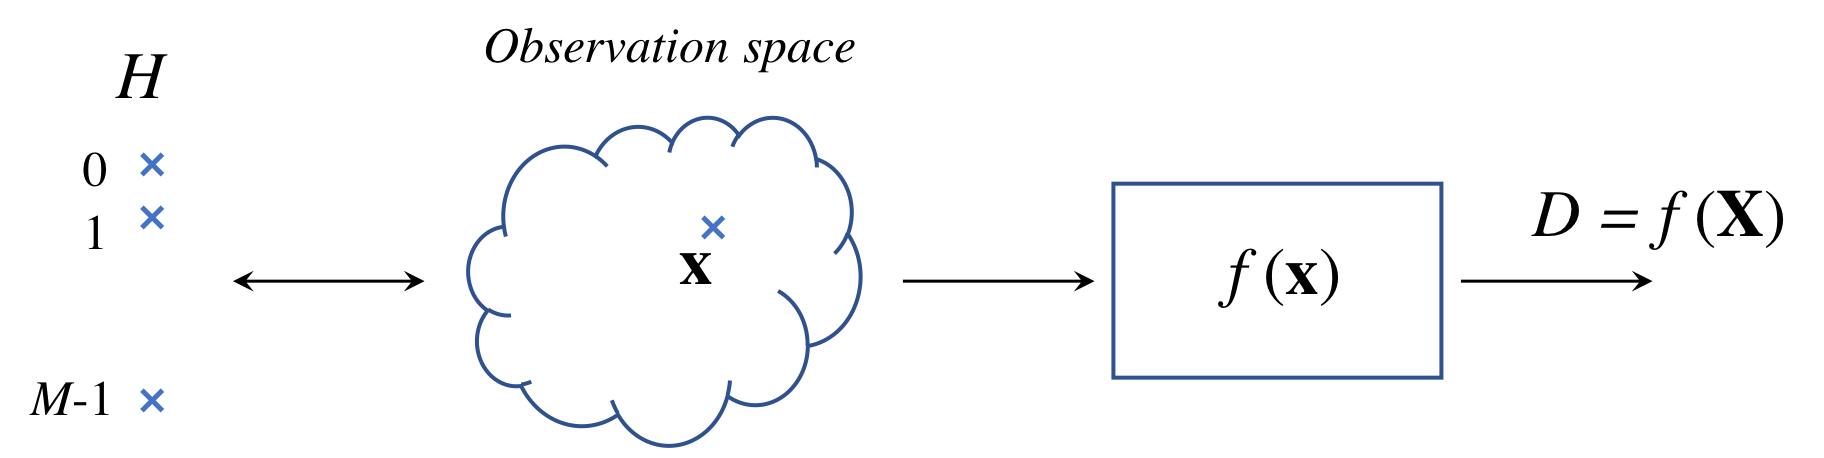
\includegraphics[width=10cm]{Figures//classification_overview.png}
\end{center}
\caption{Diagram block of hypothesis testing problems.\label{fig:clas_overview}}
\end{figure}

In this context, a \textbf{detector} is a function that, for any input $\mathbf{x}\in \mathcal{X}$, outputs a \emph{decision} $d=f(\mathbf{x})\in \{0, 1, \ldots M-1\}$, i.e., it makes a guess on the value of the true hypothesis. Depending on the application scenario, the detector receives another names, like \textbf{decision-maker} or \textbf{classifier}. In this chapter we will take these terms as synonymous.

We should make a few considerations about the functions $f({\bf x})$ that we admit as valid detectors in this course:

\begin{itemize}
\item Funcion $f(\cdot)$ is \emph{deterministic}. This implies that if the same vector is presented several times, the function will output the same value each time. Irrespective of this, when the input is a random vector, $D=f(\bf X)$ is a random variable.
\item The function is surjective, that is, every input ${\bf x}$ generates one and only one output, but different inputs can generate the same output. Hence, the function divides the observation space into $M$ non-overlapping regions, ${\cal X}_d$, $d = 0, 1, \ldots M-1$, i.e., one region per hypotheses. The boundaries between regions are known as \textit{decision boundaries}.
\end{itemize}

\begin{example}
The detector $f(x) = u(x^2 -1)$, where $u(\cdot)$ is the step function, is defined for any $x$ on the real line, and is characterized by the following decision regions:
\begin{align}{\cal X}_0 & = \left\{ x \in \Re | x^2-1 < 0\right\} = (-1,1), \nonumber\\
{\cal X}_1 & = \left\{ x \in \Re | x^2-1 \geq 0\right\} = (-\infty,-1] \cup [1,\infty). \nonumber
\end{align}
where we have assumed $u(0)=1$. In this example, the regions are connected and non-empty.
\end{example}

\begin{example}
\label{ex:decisionregions}
The detector $f({\bf x}) = \arg\min_i y_i({\bf x})$ defined over ${\cal X} = [0,1]^2$, with
\begin{align}
y_0({\bf x}) & = \|{\bf x}\|^2, \nonumber \\
y_1({\bf x}) & = x_1 - x_0 +1, \nonumber \\
y_2({\bf x}) & = x_0 - x_1 + 1, \nonumber 
\end{align}
is characterized by the decision regions depicted in Fig. \ref{fig:decisionregions}.

%\begin{figure}
\begin{center}
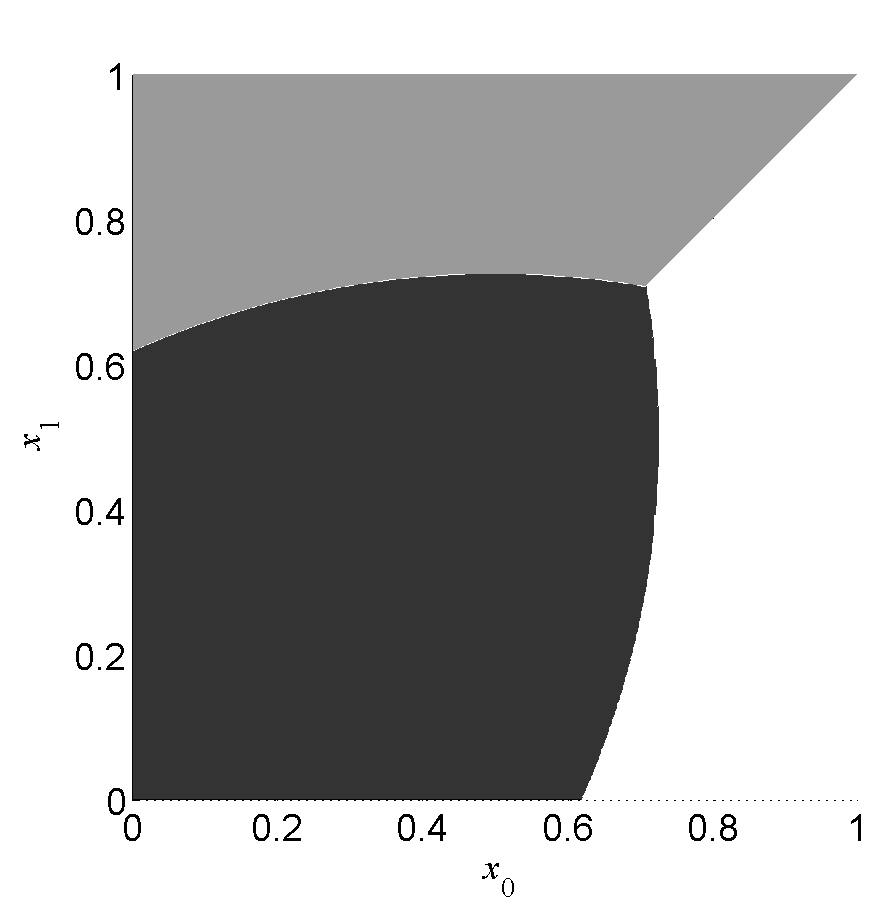
\includegraphics[width=6cm]{Figures//DecRegEx.pdf}
\end{center}
\captionof{figure}{Decision regions for the detector given in Example \ref{ex:decisionregions}: ${\cal X}_0$ (black), ${\cal X}_1$ (grey), and ${\cal X}_2$ (white).\label{fig:decisionregions}}
%\end{figure}
    
\end{example}

%%%%%%%%%%%%%%%%%%%%%%%%%%%%%%%%%
\subsection{Modeling uncertainty}
\label{subsec:statistical_info}

We review now the main distributions that will be employed in detection problems:
\begin{itemize}
\item {\em A priori} probability distribution of the hypotheses: This is a discrete distribution that quantifies the probability of each hypothesis independently of the observations. If we did not have access to any observation, the decision-maker should rely entirely on these probabilities.  %, (see example in Section \ref{subsec:example1}),
$$P_H(h), \qquad \text{ for } \quad h = 0, 1, \ldots,\;M-1.$$
    
\item Likelihood of the hypotheses: \textcolor{blue}{the conditional distribution of the observation, given the hypothesis. For a continuous observation variable, it is given by a probability density function, $$p_{{\bf X}|H}({\bf x}|h) \qquad \text{ for } \quad {\bf x} \in {\cal X},$$
for each hypothesis $h = 0, 1, \ldots,\; M-1$. Note that the domain of each distribution may depend on the hypothesis}.
    
\item {\em A posteriori} distribution of the hypotheses:
$$P_{H|{\bf X}}(h|{\bf x}), \qquad \text{ for } \quad h = 0, 1, \ldots,\; M-1.$$
\textcolor{blue}{It is a probability measure of the uncertainty about the hypothesis after the observation ${\bf X}={\bf x}$. This distribution plays a fundamental role for the statistical design of detectors.}
\end{itemize}

{\em A priori} and {\em a posteriori} probabilities are related by Bayes' Theorem, which states
    $$P_{H|{\bf X}}(h|{\bf x}) = \frac{p_{{\bf  X} | H}({\bf x}|h) P_H(h)}{p_{\bf X}({\bf x})}.$$
Bayes' Theorem shows how \textcolor{blue}{to update the probabilities of the hypotheses in light of the observation ${\bf X}={\bf x}$.} Note that if we know both the {\em a priori} probabilities of the hypothesis and their likelihoods, the joint distribution of $\bf X$ and $H$ can be calculated. The joint distribution is the most complete characterization of the random variables, and from it any other probability function can be calculated as well.

In the following, we consider two different kinds of problems involving $M$-ary hypothesis testing problems:
\begin{itemize}
\item Analysis of detectors: Here, the detector is given, and the objective is to analyze its performance with respect to certain performance metrics.
\item Detector design: The goal is to build a function $f(\bf x)$ to optimize a desired performance metric.
\end{itemize}

%%%%%%%%%%%%%%%%%%%%%%%%%%%%%%%%%%%%%%%%%%%%%%%
\section{Performance metrics}
\label{subsec:analysis}
%%%%%%%%%%%%%%%%%%%%%%%%%%%%%%%%%%%%%%%%%%%%%%%

The first problem that we consider is the evaluation of the performance of a given detector. In this section, we review different metrics that can be used to assess performance. In all cases, we consider first the multiple hypothesis test scenario, and afterwards we specialize it to the binary case.

%%%%%%%%%%%%%%%%%%%%%%%%%%%%%%%%%
\subsection{Probability of error}

The probability of error is the probability of a wrong decision, i.e., the output of the detector is not equal to the true hypothesis. Under a frequentist approach, it can be interpreted as the average number of \textcolor{blue}{decision errors after a infinite sequence of independent observations. It can be computed from the likelihood functions and the prior probabilities as}
\begin{align}
    P_e = \{D\neq H\} & = 1 - P\{D=H\} \nonumber \\
    & = 1 - \sum_{h=0}^{M-1} P\{D=h, H=h\} \nonumber \\
    & = 1 - \sum_{h=0}^{M-1} P\{D=h| H=h\} P_H(h) \nonumber \\
    & = 1 - \sum_{h=0}^{M-1} P_H(h) \int_{{\cal X}_h} p_{{\bf X}|H}({\bf x}|h) d{\bf x},\nonumber
\end{align}
where we have exploited that the probability of error is one minus the probability of correct decision, or \textbf{accuracy}. This is, in most cases, more convenient since the number of combinations where $D$ and $H$ are equal is (much) smaller than the number of combinations where they differ. Moreover, the last line of the previous expression follows from
$$P(D=h| H=h) = P({\bf x}\in {\cal X}_d| H=h) = \int_{{\cal X}_h} p_{{\bf X}|H}({\bf x}|h) d{\bf x},$$
which states that, conditioned on $H=h$, the probability of $D=h$ is precisely the integral of the likelihood of that hypothesis in the region where the given detector decides in favor of hypothesis $h$, i.e., ${\cal X}_h$.

The \emph{conditional} probability of error for a particular observation vector ${\bf x} \in {\cal X}_d$ can be computed as
\begin{equation}
P\{H\neq d|{\bf x}\} = 1 - P\{H = d|{\bf x}\} = 1 - P_{H|{\bf X}}(d|{\bf x}) 
                     = \sum_{\substack{l = 0 \\ l \neq d}}^{M-1} P_{H|{\bf X}}(l|{\bf x})
\label{eq:Pe_x}
\end{equation}
In other words, the probability of error at a particular ${\bf x} \in {\cal X}_d$ is the sum of the {\em a posteriori} probabilities of hypothesis different from $d$ conditioned on this particular observation. 
%For instance, imagine that in a three-hypothesis testing problem for a given ${\bf x}_o$ a detector selects hypothesis $0$. Then, the probability of error for  ${\bf x}_o$ is the sum of the probabilities of hypothesis $1$ and $2$ conditioned on ${\bf X} = {\bf x}_o$, i.e., the sum of {\em a posteriori} probabilities $P_{H|{\bf X}}(1|{\bf x}_o)$ and $P_{H|{\bf X}}(2|{\bf x}_o)$.

%%%%%%%%%%%%%%
\subsubsection{Binary case: $P_e$, $\pfa$, $\pmis$ and $\pdet$}
For the binary case, contrary to the multiple hypotheses test, computing the probability of error  involves as many terms as the probability of a correct decision since
\begin{align}
P_e & = P\{D=0, H=1\} + P\{D=1, H=0\} \nonumber \\
    & = P\{D=0|H=1\} P_H(1) + P\{D=1|H=0\} P_H(0). \nonumber
\end{align}
In the expression above we find two terms that are normally referred to as the \textbf{probability of false alarm} (also known as probability of \emph{Type I error} or \emph{significance level}) and the \textbf{probability of missing} (or probability of \emph{Type II} error):
\begin{align}
\pfa  & = P\{D=1|H=0\} = \int_{{\cal X}_1} p_{{\bf X}|H}({\bf x}|0) d{\bf x}, \nonumber \\
\pmis & = P\{D=0|H=1\} = \int_{{\cal X}_0} p_{{\bf X}|H}({\bf x}|1) d{\bf x}. \nonumber
\end{align}
Similarly, the \textbf{probability of detection} (\emph{power} or \emph{sensitivity}) is defined as
$$P_\text{D} = P\{D=1|H=1\} = 1 - P_\text{M},$$
and
$$P\{D=0|H=0\} = 1 - \pfa,$$
is the \textbf{specificity}. Using these definitions, the probability of error can now be expressed more compactly as
$$P_e = P_\text{M} P_H(1) + P_\text{FA} P_H(0).$$
Interestingly, for the computation of $P_\text{FA}$ and $P_\text{M}$, only likelihoods are required. However, in order to compute the overall probability of error, we also need to know the {\em a priori} probabilities of the hypothesis.

%%%%%%%%%%%%%%%%%%%%%%%%%%%%%%%%%%%%%%%%%%%%%%%%%%%%
\subsection{Receiver Operating Characteristic (ROC)}

We also introduce here an important concept for the analysis of binary hypothesis tests: the receiver operating characteristic (ROC) curve. The ROC curve plots the probability of false alarm, $P_\text{FA}$, against the probability of detection, $P_\text{D}$ for different values of some parameter. Figure \ref{fig:ROC} shows the ROC curves of two different detectors, Detector 1 and Detector 2. As can be seen in this figure, the performance of Detector 2 is clearly better than that of Detector 1, since for each $P_\text{FA}$, the $P_\text{D}$ of Detector 2 is equal or larger than that of Detector 1. Moreover, both detectors perform better than a random decision whose ROC curve is also shown in the figure. One final comment is in order. For almost all detectors it is not possible to increase the probability of detection without increasing the probability of false alarm.

\begin{figure}
\begin{center}
\includestandalone{Figures/ROC}
\end{center}
\caption{ROC curves for two different detectors.\label{fig:ROC}}
\end{figure}

%%%%%%%%%%%%%%%%%
\subsection{Risk}

In scenarios where the consequences of each type of error are different, the probability of error is not an adequate performance measure. Imagine, for instance, a detector that discriminates whether there are or not suspicious tumor masses in a medical image. Such detector is used as a pre-diagnosis system, so that patients that can have a tumor are then explored with more accurate (but also invasive) techniques. In this case, there is a clear asymmetry between both kinds of errors: The incorrect decision that tumor masses are present would result in an unnecessary biopsy and inconvenience for the patient, but the opposite error could delay the diagnosis until a time when the process is irreversible.

To assign a penalty to different kinds of errors, we can define a cost function \textcolor{blue}{$c(d, h)$, or 
$$c_{dh}, \qquad d,h = 0, \ldots, M-1,$$
whose value is the cost of deciding $D=d$ when the true hypothesis is $H=h$}. In general, we will assume that the cost for each particular $d$ and $h$ is deterministic. However, the cost $c_{DH}$, as a function of the random variables $D$ and $H$, is a random variable, too. 
Given a detector $D = \phi({\bf X})$, we define the \textbf{risk} $R_\phi$ as the expected value of the cost,
\begin{align}
\label{eq:def_Drisk}
R_\phi = \EE\left\{c_{DH}\right\} = \sum_{h=0}^{M-1} \sum_{d=0}^{M-1} c_{dh} P_H(h) P_{D|H}(d|h).
\end{align}

Since $\phi(\mathbf{x})=d$ when the observation belongs to the decision region of $D=d$, that is, $\mathbf{x} \in \mathcal{X}_d$, the conditional probabilities $P_{D|H}(d|h)$ can be calculated as
\begin{align}
\label{eq:PDgivenH}
P_{D|H}(d|h) = P\{X \in \mathcal{X}_d | H=h \}
             = \int_{\mathcal{X}_d} p_{\mathbf{X}|H}(\mathbf{x}|h) d\mathbf{x}
\end{align}
therefore
\begin{align}
R_\phi 
	& = \sum_{h=0}^{M-1} P_H(h) \sum_{d=0}^{M-1} c_{dh} 
	                     \int_{{\bf x}\in {\cal X}_d} p_{{\bf X}|H}({\bf x}|h) d{\bf x}.
\end{align}

%%%%%%%%%%%%%%%
\begin{example} \label{ex_dec1}
Consider a multiclass decision problem with three hypotheses whose likelihoods are:
$$\begin{array}{lll}
p_{X|H}(x|0)= & 1 &  \quad 0<x<1 \\ 
p_{X|H}(x|1)= & 2(1-x)  &  \quad 0<x<1 \\ 
p_{X|H}(x|2)= & 2x & \quad 0<x<1 
\end{array} $$
knowing that the prior probabilities of the hypotheses are: $P_H(0)=0.4$ and $P_H(1)=P_H(2)=0.3$, and the cost policy is given by $c_{hh}=0, \; h=0,1,2$ and $c_{hd}=1, \; h \neq d$. Obtain the risk of the decision-maker:
$$ \phi (x) = \left\lbrace  \begin{array}{ll}    
1, & \quad x<0.5 \\
2, & \quad x>0.5 
\end{array} 
\right. $$

Applying the expression \eqref{eq:def_Drisk} to this problem we have:
$$\begin{array}{rl}
R_\phi = &  c_{10} P_H(0) P_{D|H}(1|0) + c_{20} P_H(0) P_{D|H}(2|0) + c_{01} P_H(1) P_{D|H}(0|1) \\
& +  c_{21} P_H(1) P_{D|H}(2|1) +  c_{02} P_H(2) P_{D|H}(0|2) +   c_{12} P_H(2) P_{D|H}(1|2) 
\end{array} $$
where the terms $P_{D|H}(d|h)$ can be calculated using \eqref{eq:PDgivenH}
$$\begin{array}{ll}
P_{D|H}(0|1) &=P_{D|H}(0|2)= 0  \\
P_{D|H}(1|0) &= \int_{{\cal X}_1} p_{{X}|H}({x}|0) \;d{x} = \int_{0}^{0.5} 1 \;d{x} = 0.5 \\ 
P_{D|H}(2|0) &= \int_{{\cal X}_2} p_{{X}|H}({x}|0)\; d{x} = \int_{0.5}^{1} 1 \;d{x} = 0.5 \\
P_{D|H}(1|2) &=\int_{{\cal X}_1} p_{{X}|H}({x}|2) \;d{x} = \int_{0}^{0.5} 2x \;d{x} = 0.25 \\
P_{D|H}(2|1) &=\int_{{\cal X}_2} p_{{X}|H}({x}|1) \;d{x} = \int_{0.5}^{1} 2(1-x) \;d{x} = 0.25 
\end{array} $$
and substituting these, we arrive at
$$\begin{array}{rl}
R_\phi = &  0.4 \cdot 0.5  + 0.4 \cdot 0.5 + 0.3 \cdot 0.25 + 0.3 \cdot 0.25 = 0.55
\end{array} $$
\end{example}
\vspace{0.2cm}
%%%%%%%%%%%%%%

Finally, we define the \textbf{conditional risk} as the expected cost conditioned on a given value of ${\bf x}$, $\EE\left\{c_{dH}\right|{\bf x}\}$. Taking into account that, for a given ${\bf x}$ and a given detector, the decision value is fixed, it is only required to take expectations with respect to such hypothesis. The conditional risk for a given observation ${\bf x} \in {\cal X}_d$ is given by
\begin{equation}
\EE\left\{ c_{dH}\right|{\bf x}\} = \sum_{h=0}^{M-1} c_{dh} P_{H|X}(h|{\bf x}).
\label{eq:cost_x}
\end{equation}

%%%%%%%%%%%%%%%
\begin{example} \label{ex_dec2}
Continuing with Example \ref{ex_dec1}, the conditional risk of each decision can be calculated as:
$$\EE\{c(d,H)|x\}=  c_{d0} P_{H|X}(0|x) +  c_{d1} P_{H|X}(1|x) + c_{d2} P_{H|X}(2|x) $$
where the posterior distributions can be obtained by applying Bayes' Theorem:
\begin{align*} 
P_{H|X}(0|x) =& \frac{p_{X|H}(x|0) P_H(0)}{\sum_{h=0}^2 p_{X|H}(x|h) P_H(h) } 
             =  \frac{1 \cdot 0.4} { 1 \cdot 0.4 + 2(1-x) \cdot 0.3 + 2x \cdot 0.3} 
             =  0.4 \\ 
P_{H|X}(1|x) =& \frac{p_{X|H}(x|1) P_H(1)}{\sum_{h=0}^2 p_{X|H}(x|h) P_H(h) } 
             =  \frac{2(1-x)\cdot 0.3} { 1 } =0.6(1-x) \\ 
P_{H|X}(2|x) =& \frac{p_{X|H}(x|2) P_H(2)}{\sum_{h=0}^2 p_{X|H}(x|h) P_H(h) } = \frac{2x\cdot 0.3} {1} =0.6x 
\end{align*}

This leads to:
\begin{itemize}
\item if $d=0$:
$$\begin{array}{rl} 
\EE\{c_{0,H}|x\} =& c_{00} P_{H|X}(0|x) +  c_{01} P_{H|X}(1|x) + c_{02} P_{H|X}(2|x) \\
                 =& 0 \cdot 0.4+ 1 \cdot 0.6(1-x) + 1 \cdot 0.6x= 0.6 
\end{array}$$
\item if $d=1$:
$$\begin{array}{rl} 
\EE\{c_{1,H}|x\} =& c_{10} P_{H|X}(0|x) +  c_{11} P_{H|X}(1|x) + c_{12} P_{H|X}(2|x) \\
                 =& 1 \cdot 0.4+ 0 \cdot 0.6(1-x) + 1 \cdot 0.6x= 0.4+0.6x 
\end{array}$$
\item if  $d=2$:
$$\begin{array}{rl} 
\EE\{c_{2,H}|x\} =& c_{20} P_{H|X}(0|x) +  c_{21} P_{H|X}(1|x) + c_{22} P_{H|X}(2|x) \\
                 =& 1 \cdot 0.4+ 1 \cdot 0.6(1-x) + 0 \cdot 0.6x=  1-0.6x 
\end{array}$$
\end{itemize} 
\end{example}
%%%%%%%%%%%%%

%%%%%%%%%%%%%%
\subsubsection{Binary case: risk}

For the binary case, a simpler expression can be obtained in terms of $\pfa$, $\pmis,$ and $\pdet$ as follows
\begin{align}
\label{eq:bin_risk}
R_\phi 
    &= c_{00} P(D=0, H=0) + c_{01} P(D=0,H=1)                    \nonumber\\
    %& \;\;\;\;\;\; + c_{10} P(D=1, H=0) + c_{11} P(D=1,H=1)        \nonumber\\
    &= c_{00} P(D=0|H=0) P_H(0) + c_{01} \pmis P_H(1) + c_{10} \pfa P_H(0) + c_{11} \pdet P_H(1) .      \nonumber\\
    &= c_{00} (1-\pfa) P_H(0) + c_{01} \pmis P_H(1) + c_{10} \pfa P_H(0) + c_{11} (1-\pmis) P_H(1) .\nonumber\\
    &= \left(c_{00} P_H(0) + c_{11} P_H(1)\right) + (c_{01}- c_{11}) \pmis P_H(1) + (c_{10}-c_{00}) \pfa P_H(0) 
\end{align}
The previous expression shows that the risk of a decision-maker is the sum of three components:
\begin{itemize}
\item $(c_{00} P_H(0) + c_{11} P_H(1))$ is the minimum risk of the ideal decision-maker, the one with $\pmis=0$ and $\pfa=0$ who succeeds with probability 1.
\item $(c_{01}-c_{11}) P_H(1) \pmis$ is the increase in risk caused by miss errors.
\item $(c_{10}-c_{00}) P_H(0) \pfa$ is the increase in risk caused by false alarms.
\end{itemize}
Note that the ideal decision-maker is, in general, unachievable, because if the likelihoods of the hypotheses overlap, it is not possible to avoid errors. The optimal decision-maker will be the one who finds a good compromise between miss errors and false alarms, such that the risk in (\ref{eq:bin_risk}) is minimized.


%%%%%%%%%%%%%%%%%%%%%%%%%
\section{Detector design}
\label{subsec:design}
%%%%%%%%%%%%%%%%%%%%%%%%%

Once we have studied different ways of analyzing the performance of a given detector, we turn our attention to the problem of designing detectors that maximize one of these performance metrics.

%%%%%%%%%%%%%%%%%%%%%%%%%%%%%%%%%%%%%%%%%%%%%%%%%%%%%%%%%%%%%%%%%%%%%%%%%
\subsection{Maximum likelihood and maximum \emph{a posteriori} detectors}

A first possibility would be to rely directly on the maximization of the available probability density functions:

\begin{itemize}
\item The detector that maximizes the likelihood is known as the {\em maximum likelihood} (ML) detector:
    $$d_{ML} = \arg\max_h p_{{\bf X}|H}({\bf x}|h).$$
\item The detector that selects the hypothesis with maximum {\em a posteriori} probability is known as the  maximum {\em a posteriori} (MAP) detector:
    $$d_{MAP} = \arg\max_h P_{H|{\bf X}}(h|{\bf x}).$$
\end{itemize}

Finally, there are two properties that are worth considering with respect to these detectors:
\begin{enumerate}
    \item When the {\em a priori} probabilities of the hypothesis are the same, i.e., $P_H(h) = 1/M$, the ML and MAP detectors are identical. This can be shown from the Bayes' Theorem, since in this case
    $$d_{MAP} = \arg\max_h P_{H|{\bf X}}(h|{\bf x}) = \arg\max_h \frac{p_{{\bf X}|H}({\bf x}|h) P_H(h)}{p_{\bf X}(\bf x)} = \arg\max_h p_{{\bf X}|H}({\bf x}|h) = d_{ML}.$$
    
    \item The MAP detector minimizes the probability of error. Note that according to \eqref{eq:Pe_x} the probability of error for a given $\bf x$ can be expressed as
    $$P(D\neq H|{\bf x}) = 1 - P_{ H|{\bf X}}(h|{\bf x}).$$
    Since the MAP detector selects, for every $\mathbf{x}$, the hypothesis maximizing $P_{H|{\bf X}}(h|{\bf x})$, it minimizes the conditional error probability $P(D\neq H|{\bf x})$. Since the overall error probability is an integral over the conditional error probabilities, i.e.,
    $$P(D\neq H) = \int_{\mathcal{X}} P(D\neq H|{\bf x}) p_{\bf X}(\bf x) d{\bf x},$$
the MAP detector minimizes the overal probability of error, too.
    
\end{enumerate}

%%%%%%%%%%%%%%%%%%%%%%%%%%%%%%%%%%%%%%%%%%%%%%%%%
\subsubsection{Binary case: ML and MAP detectors}

The expressions of the ML and MAP detectors become fairly simple for the binary case:
\begin{itemize}
\item Maximum likelihood detector:
$$p_{{\bf X}|H}({\bf x}|1) \dunodcero p_{{\bf X}|H}({\bf x}|0),$$
which can be expressed as a {\em likelihood ratio test} (LRT)
\begin{align*}
\label{eq:ML_LRT}
\frac{p_{{\bf X}|H}({\bf x}|1)}{p_{{\bf X}|H}({\bf x}|0)} \dunodcero 1,
\end{align*}
where we have taken into account that the likelihoods are non-negative. Sometimes, it will be more convenient to work with the {\em log-likelihood ratio test} (LLRT)
\begin{equation}
\label{eq:LLRT}
\log \left[ \frac{p_{{\bf X}|H}({\bf x}|1)}{p_{{\bf X}|H}({\bf x}|0)} \right] 
	= \log p_{{\bf X}|H}({\bf x}|1) - \log p_{{\bf X}|H}({\bf x}|0) \dunodcero 0,
\end{equation}
which can be done because the logarithm is a monotonically increasing function.
\item Maximum \emph{a posteriori} detector:
$$p_{H|{\bf X}}(1|{\bf x}) \dunodcero p_{H|{\bf X}}(0|{\bf x}),$$
which can also be expressed as a LRT as
\begin{align} 
\frac{p_{{\bf X}|H}({\bf x}|1)}{p_{{\bf X}|H}({\bf x}|0)} 
	\dunodcero \frac{P_H(0)}{P_H(1)}.
\end{align}
\end{itemize}

As in the general case with $M$ hypothesis, the MAP detector minimizes the probability of error and the ML and MAP detectors are the same if $P_H(0)=P_H(1)=0.5$. Moreover, we can see that both detectors can be expressed as a LRT
\begin{align} 
\label{eq:def_LRT}
\frac{p_{{\bf X}|H}({\bf x}|1)}{p_{{\bf X}|H}({\bf x}|0)} \dunodcero \eta,
\end{align}
where $\eta$ is a threshold. When this threshold is $1$, the LRT is the ML detector and for $\eta = P_H(0)/P_H(1)$, the LRT becomes the MAP detector, that is, minimum $P_e$ detector. Hence, we get two different points in the ROC curve. Actually, sweeping the value of the threshold generates the complete ROC curves in Figure \ref{fig:ROC}.\footnote{This actually applies to all detectors that can be written as $\phi({\bf x}) \dunodcero \eta$. That is, comparing a function of the observations with a threshold achieves a given $(P_\text{FA},P_\text{D})$ point in the ROC curve. These detectors are known as threshold detectors.}



%%%%%%%%%%%%%%%%%%%%%%%%%%%%%%%%%%%%%%%%%%%%%%%%%%%%%%%%%%%%%%%%
\subsection{Bayesian decision-making: the minimum risk detector}

As we have already studied, sometimes it makes more sense to measure the performance of a detector in terms of the expected cost. Therefore, it is important to tackle the problem of designing a detector that is optimum with respect to the expected cost.

Remember that the expected cost of a detector deciding $d$ for an observation ${\bf x}$ is given by Equation \eqref{eq:cost_x}, which we reproduce here for convenience:
\begin{equation}
   \EE\left\{ c_{dH}\right|{\bf x}\} = \sum_{h=0}^{M-1} c_{dh} P_{H|\bf X}(h|{\bf x}) \label{eq:mean_x_2}.
\end{equation}
Minimizing the expected cost over the whole observation space requires that decisions for each observation minimize the conditional expected cost. That is, for each ${\bf x}$ the above expression should be minimized, and the expression of the minimum mean cost detector can be stated as follows:
$$d^\star = \arg\min_{d} \sum_{h=0}^{M-1} c_{dh} P_{H|\bf X}(h|{\bf x}).$$
Hence, when designing the detector, we need to evaluate the cost of the different decisions for each observation vector, and select the decision for which the expected cost is minimized.

%%%%%%%%%%%%%%%
\begin{example} \label{ex_dec2}
Continuing with Example \ref{ex_dec2}, since
\begin{align*}
\EE\{c_{0,H}|x\} =& 0.6   \\
\EE\{c_{1,H}|x\} =& 0.4+0.6x  \\
\EE\{c_{2,H}|x\} =& 1-0.6x 
\end{align*}
(as shown in the figure), the Bayesian detector is
\begin{align*}
D = \begin{cases}
	1 & 0       \le X \le \frac13 \\
	0 & \frac13 \le X \le \frac23 \\
	2 & \frac23 \le X \le 1 
	\end{cases}
\end{align*}
% Requires in the preamble:
% \usepackage{pgfplots}
% \pgfplotsset{compat=1.18}

\begin{center}
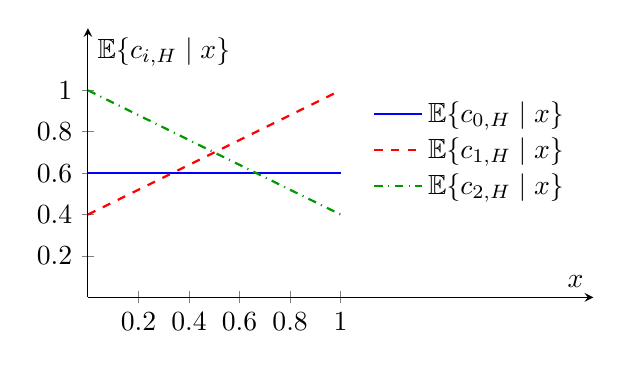
\begin{tikzpicture}
\begin{axis}[
    width=8cm,
    height=5cm,
    domain=0:1,
    samples=200,
    axis lines=middle,     % only horizontal and vertical axes
    xmin=0, xmax=2,
    ymin=0, ymax=1.3,
    xlabel={$x$},
    ylabel={$\EE\{c_{i,H}\mid x\}$},
    xtick={0,0.2,0.4,0.6,0.8,1},
    ytick={0,0.2,0.4,0.6,0.8,1},
    enlargelimits=false,
    clip=false,
    legend style={
        at={(0.97,0.77)},
        anchor=north east,
        draw=none,
        fill=white
    }
]
\addplot[blue, solid, thick] {0.6};
\addlegendentry{$\mathbb{E}\{c_{0,H}\mid x\}$}
\addplot[red, dashed, thick] {0.4 + 0.6*x};
\addlegendentry{$\mathbb{E}\{c_{1,H}\mid x\}$}
\addplot[green!60!black, dashdotted, thick] {1 - 0.6*x};
\addlegendentry{$\mathbb{E}\{c_{2,H}\mid x\}$}

\end{axis}
\end{tikzpicture}
\end{center}
\end{example}
%%%%%%%%%%%%%

It is interesting to point out that when the cost function penalizes equally all kinds of errors, i.e.,
$$c_{dh} = \left\{\begin{array}{ll} 0, & \;\;\;\;d=h \\ c, & \;\;\;\;d\neq h\end{array}\right.$$
the detector with minimum risk is MAP. This is easily proved by replacing these costs into the expression for the minimum expected cost detector
\begin{align*}
d^\star & = \arg\min_{d} \sum_{h=0}^{M-1} c_{dh} P_{H|\bf X}(h|{\bf x})  \\
        & = \arg\min_{d} \ c \sum_{h\neq d} P_{H|\bf X}(h|{\bf x})       \\
        % & = \arg\min_{d} \sum_{h\neq d} P_{H|\bf X}(h|{\bf x})         \\
        & = \arg\min_{d} \left\{1 - P_{H|\bf X}(d|{\bf x})\right\}       \\
        & = \arg\max_{d} P_{H|\bf X}(d|{\bf x})                          \\
        & = d_{MAP}.
\end{align*}


%%%%%%%%%%%%%%%
\subsubsection{Binary case: Minimum risk detector}

In the binary case, we can also express the optimum detector with respect to a cost function as a LRT. Let us start by particularizing \eqref{eq:mean_x_2} for $d=0$ and $d=1$, and then follow the criterion of deciding in favor of the minimum cost, i.e.,
$$\mathbb{E}\left\{ c_{0H}\right|{\bf x}\} \dunodcero \mathbb{E}\left\{ c_{1H}\right|{\bf x}\}.$$
Now, using the definition of expectation, the criterion becomes
$$c_{00}P_{H|{\bf X}}(0|{\bf x}) + c_{01} P_{H|{\bf X}}(1|{\bf x})\dunodcero c_{10}P_{H|{\bf X}}(0|{\bf x}) + c_{11} P_{H|{\bf X}}(1|{\bf x}),$$
which after some algebra can be rewritten as
$$\displaystyle\frac{P_{H|{\bf X}}(1|{\bf x})}{P_{H|{\bf X}}(0|{\bf x})}\dunodcero \displaystyle\frac{c_{10}-c_{00}}{c_{01}-c_{11}}.$$
Finally, using Bayes' Theorem, we may rewrite the \emph{a posteriori} probabilities in terms of the likelihoods and the \emph{a priori} probabilities, which finally yields
$$\displaystyle\frac{P_{{\bf X}|H}({\bf x}|1)}{P_{{\bf X}|H}({\bf x}|0)}\dunodcero \displaystyle\frac{c_{10}-c_{00}}{c_{01}-c_{11}} \displaystyle\frac{P_H(0)}{P_H(1)},$$
and corresponds to yet another point of the ROC curve of the LRT.


%%%%%%%%%%%%%%%%%%%%%%%%%%%%%%%%%%%
\subsection{Non-Bayesian detectors}

Non-Bayesian detectors are those that do not ground on a probability model for the hypothesis. Their design depends on the likelihood functions only. This is the case, for instance, of the ML detector. Other non-Bayesian detectors, in the binary case can be expressed as the LRT in \eqref{eq:def_LRT} for different valures of $\eta$. The Neyman-Pearson detector is a classical example.


%%%%%%%%%%%%%%
\subsubsection{Binary case: Neyman-Pearson detector}

The Neyman-Pearson (NP) detector is a well known detector for binary problems which maximizes the probability of detection while it provides a bound on the probability of false alarm. Before proceeding with the derivation, let us recall the definitions of probability of false alarm and detection
\begin{align}
\pfa  & = \int_{{\cal X}_1} p_{{\bf X}|H}({\bf x}|0) d{\bf x}, \nonumber \\
\pdet & = \int_{{\cal X}_1} p_{{\bf X}|H}({\bf x}|1) d{\bf x}. \nonumber
\end{align}
The NP detector can be derived as the solution of the following constrained optimization problem:
\begin{equation*}
\text{maximize } P_\text{D}, \quad \text{subject to } P_\text{FA} \le \alpha,
\end{equation*}
The solution to this kind of problems is obtained from the Lagrangian, $\mathcal{L}(\mathcal{X}_1, \eta)$, defined as:
\begin{align}
\mathcal{L}(\mathcal{X}_1, \eta) 
	&= \pdet - \eta (\pfa - \alpha) \nonumber \\
    &= \int_{\mathcal{X}_1} p_{\X|H}(\x |1) d\x 
     - \eta \left( \int_{\mathcal{X}_1} p_{\X|H}(\x |0) d\x - \alpha \right)    
    \nonumber \\
    &= \int_{\mathcal{X}_1} \left(p_{\X|H}(\x|1) - \eta p_{\X|H}(\x|0) \right) d\x 
     + \eta \alpha.
\end{align}
Note that the optimization variable is the decision region $\mathcal{X}_1$ (the set of observations where we decide $D=1$). To maximize the Lagrangian, we must choose $\mathcal{X}_1$ such that we include all points $\mathbf{x}$ where the integrand is non-negative:
\begin{equation*}
\mathcal{X}_1 
	= \{ \x \mid p_{\X|H}(\x|1) - \eta p_{\X|H}(\x|0) \geq 0 \}.
\end{equation*}

This result leads directly to the Likelihood Ratio Test (LRT):
\begin{equation*}
\Lambda(\mathbf{x}) 
	= \frac{p_{\X|H}(\x|1)}{p_{\X|H}(\x|0)} \dunodcero \eta,
\end{equation*}
where the threshold $\eta$ is selected to achieve the desired probability of false alarm $\alpha$.

In practice, when the ROC of the LRT is a continuous function, the NP detector can be computed in two steps:
\begin{enumerate}
\item Express $\pfa$ as a function of $\eta$ for the LRT
\item Find $\eta$ such that $\pfa(\eta)=\alpha$.
\end{enumerate}


%%%%%%%%%%%%%%
\subsubsection{Minimax classifiers}

The decision rule of the MAP detector depends on the prior probability $P_H(1)$. In many practical scenarios, however, this prior is unknown or may vary, leading to a mismatch between the design prior and the true operating conditions. The minimax classifier provides a robust strategy by minimizing the maximum possible error probability.

Let $P=P_H(1)$ be the true (unknown) prior probability, and let $Q$ be the design prior used to construct the MAP detector. The resulting probability of error, $P_{\rm{e}}(P, Q)$, is a function of both. The minimax detector is found by solving:

\begin{equation}
Q^* = \argmin_{Q} \max_{P} \left[P \cdot P_\text{M}(Q) + (1-P) \cdot P_\text{FA}(Q) \right].
\end{equation}

This formulation implies that we seek a design prior $Q$ such that the detector performs well even for the "least favorable" true prior $P$. Since the error probability $P_{\rm{e}}(P, Q)$ is a linear function of $P$, the maximum error occurs at the boundaries ($P=0$ or $P=1$) unless the slope of the error function is zero. 

Therefore, the minimax solution is achieved when the error probability is independent of the true prior $P$. For binary problems, this occurs when the Likelihood Ratio Test (LRT) threshold, $\eta$ is chosen such that:
\begin{align}
\boxed{
\pfa(\eta) = \pmis(\eta)}
\end{align}
In this state, the classifier is robust: no matter how the true prior $P$ fluctuates, the error probability remains constant and equal to $\pfa$.


%%%%%%%%%%%%%%%%%%%%%%%%%%%%%%%
\section{Gaussian models}

In this section, we will derive the likelihood ratio test for Gaussian observations under several assumptions. Then, depending on the threshold, we would obtain the different detectors: NP, ML, MAP, and minimum cost.

Before proceeding, we introduce the multivariate real Gaussian probability density function (PDF), which is given by
\begin{equation*}
P_{{\bf X}}({\bf x}) = \frac{1}{(2\pi)^{N/2} |{\bf V}|^{1/2}}
\exp\left(-\frac{1}{2}({\bf x}-{\bf m})^T {\bf V}^{-1}({\bf x}-{\bf m})\right),
\label{pXGauss}
\end{equation*}
where ${\bf x}$ is an $N$-dimensional vector, ${\bf m}$ is the mean vector, and ${\bf V}$ is the cross-covariance matrix. Then, under hypothesis $h = 0$, the likelihood is
\begin{equation*}
P_{{\bf X}|H}({\bf x}|0) = \frac{1}{(2\pi)^{N/2} |{\bf V}_0|^{1/2}}
\exp\left(-\frac{1}{2}({\bf x}-{\bf m}_0)^T {\bf V}_0^{-1}({\bf x}-{\bf m}_0)\right),
\end{equation*}
whereas it is
\begin{equation*}
P_{{\bf X}|H}({\bf x}|1) = \frac{1}{(2\pi)^{N/2} |{\bf V}_1|^{1/2}}
\exp\left(-\frac{1}{2}({\bf x}-{\bf m}_1)^T {\bf V}_1^{-1}({\bf x}-{\bf m}_1)\right),
\end{equation*}
under hypothesis $h = 1$. For this hypothesis test, the LLRT in \eqref{eq:LLRT} becomes
\begin{multline*}
- \frac{1}{2}\log\left|{\bf V}_1 \right| 
- \frac{1}{2}({\bf x}-{\bf m}_1)^T {\bf V}_1^{-1}({\bf x}-{\bf m}_1) \\
+ \frac{1}{2}\log\left|{\bf V}_0 \right| 
+ \frac{1}{2}({\bf x}-{\bf m}_0)^T {\bf V}_0^{-1}({\bf x}-{\bf m}_0) 
\dunodcero \log(\eta) 
\end{multline*}
or, equivalently,
\begin{align}
({\bf x}-{\bf m}_0)^T {\bf V}_0^{-1}({\bf x}-{\bf m}_0) 
- ({\bf x}-{\bf m}_1)^T {\bf V}_1^{-1}({\bf x}-{\bf m}_1)
\dunodcero \mu
\label{eq:logLRTGauss}
\end{align}
where
\begin{equation*}
\mu = 2 \log(\eta) + \log\left|{\bf V}_1 \right| - \log\left|{\bf V}_0 \right|,
\end{equation*}
with $\eta$ being a threshold selected according to the performance criterion.

After a careful look at \eqref{eq:logLRTGauss}, it can be shown that the optimal detector in the Gaussian case is given by a second-order polynomial function. Hence, the decision boundaries\footnote{We obtain the decision boundaries for the equality in \eqref{eq:logLRTGauss}.} are quadratic surfaces. For instance, for 2D problems ($N = 2$), these boundaries are hyperbolas, parabolas, ellipses or straight lines.

In the following sections, we consider a few particular cases, and we conclude this section with two examples.

\begin{example}
	Figure \ref{fig:DecGauss2Dhip} shows the decision boundaries for the ML detector ($\eta = 1$ in \eqref{eq:logLRTGauss}), for a detection problem with 2D Gaussian observations with the following means and cross-covariance matrices:
	\begin{equation*}
	{\bf m}_0 =  \left(\begin{array}{l}  1 \\ 1 \end{array}\right), {\bf V}_0 = 
	\left(\begin{array}{ll} 1.2 & 0.43 \\ 0.43 & 1.75 \end{array} \right),
	\end{equation*}
	and
	\begin{equation*}
	{\bf m}_1 = \left(\begin{array}{l}  3 \\ 3 \end{array}\right), {\bf V}_1 = 
	\left(\begin{array}{ll} 2 & 0 \\ 0 & 1 \end{array} \right).
	\end{equation*}
	In this figure, the gray color gradient  represents the value of the likelihoods $P_{{\bf X}|H}({\bf x}|0)$ and $P_{{\bf X}|H}({\bf x}|1)$, where darker colors denote larger values. Moreover, the white curves are the iso-probability lines and the black curve is the decision boundary, which in this case is a hyperbola (the symmetric part is not shown in this figure).
	
	%\begin{figure}[htb]
		\begin{center}
			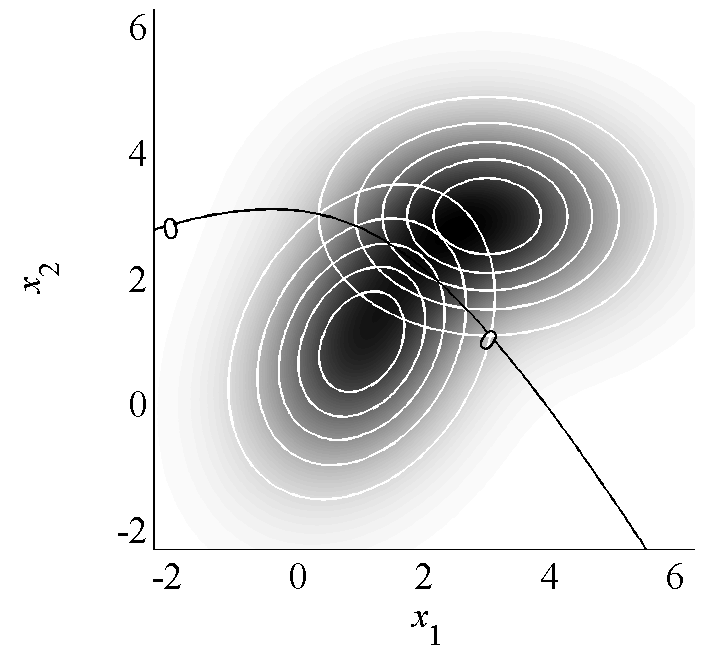
\includegraphics[width=6cm]{Figures/DecGauss2Dhip}
			\captionof{figure}{Hyperbolic decision boundary of the ML detector and likelihoods for a Gaussian detection problem with 2D observations.}
			\label{fig:DecGauss2Dhip}
		\end{center}
	%\end{figure}
\end{example}

\begin{example}
	Figure \ref{fig:DecGauss2Delip} shows an equivalent figure to that of the previous example, but for a problem with the following means and cross-covariance matrices:
		\begin{equation*}
	{\bf m}_0 =  \left(\begin{array}{l}  0\\0  \end{array}\right), {\bf V}_0 = 
	\left(\begin{array}{ll} 0.7 & 0 \\ 0 & 0.7 \end{array} \right),
	\end{equation*}
	and
	\begin{equation*}
	{\bf m}_1 = \left(\begin{array}{l}  0.2 \\ 0.4 \end{array}\right), {\bf V}_1 = 
	\left(\begin{array}{ll} 0.5 & 0 \\ 0 & 0.2 \end{array} \right).
	\end{equation*}
	In this case, the decision boundary is an ellipse.
	%\begin{figure}[htb]
		\begin{center}
			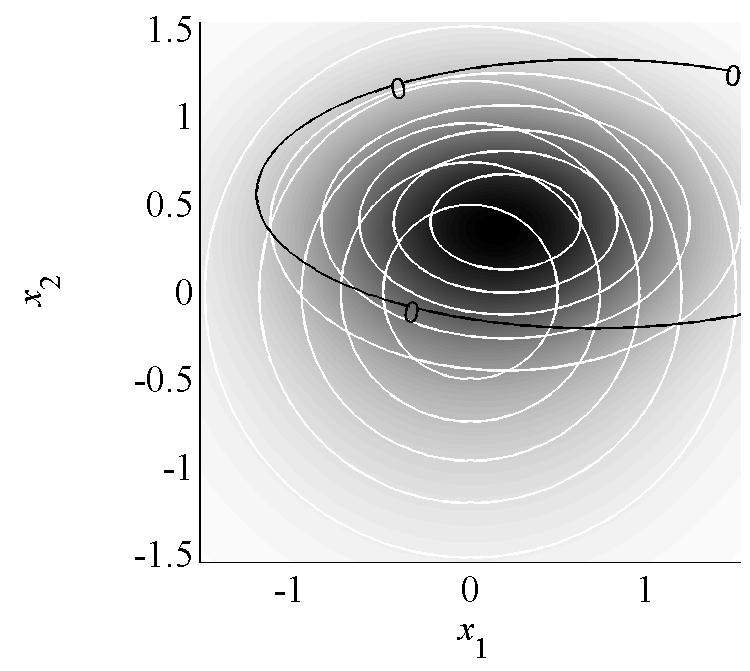
\includegraphics[width=6cm]{Figures/DecGauss2Delip.pdf}
			\captionof{figure}{Elliptic decision boundary of the ML detectors and likelihoods for a Gaussian detection problem with 2D observations.}
			\label{fig:DecGauss2Delip}
		\end{center}
	%\end{figure}
\end{example}

\subsection{Identical cross-covariance matrices}

This section considers the case of ${\bf V}_1 = {\bf V}_0 = {\bf V}$. Then, the LLRT becomes
\begin{equation*}
({\bf x}-{\bf m}_0)^T {\bf V}^{-1}({\bf x}-{\bf m}_0) 
- ({\bf x}-{\bf m}_1)^T {\bf V}^{-1}({\bf x}-{\bf m}_1)
\dunodcero \mu.
\end{equation*}
Now, expanding the quadratic forms, the above expression simplifies to
\begin{equation}
 ({\bf m}_1-{\bf m}_0)^T {\bf V}^{-1}{\bf x} \dunodcero \tilde{\mu},
 \label{eq:LLRT_Gaussian_same_Vs}
\end{equation}
where $\tilde{\mu} = \mu/2 + {\bf m}_1^T {\bf V}^{-1}{\bf m}_1/2 - {\bf m}_0^T {\bf V}^{-1}{\bf m}_0/2$. In this particular case, the LLRT in \eqref{eq:LLRT_Gaussian_same_Vs} is a linear function of the observation vector ${\bf x}$.

\begin{example}
	Figure \ref{Dec:DecGauss2Deqv} shows three decision boundaries for an example with
		\begin{equation*}
			{\bf m}_0 =  \left(\begin{array}{l}  1\\1  \end{array}\right), {\bf V}_0 = 
			\left(\begin{array}{ll} 0.44 & 0.32 \\ 0.32 & 0.81 \end{array} \right)
\end{equation*}
and
\begin{equation*}
{\bf m}_1 = \left(\begin{array}{l}  3\\3 \end{array}\right), {\bf V}_1 = 
\left(\begin{array}{ll} 0.44 & 0.32 \\ 0.32 & 0.81 \end{array} \right).
\end{equation*}
The label of each decision boundary is $\log(\eta)$. Then, $\log(\eta) = 0$ corresponds to the ML detector.
	%\begin{figure}[htb]
		\begin{center}
			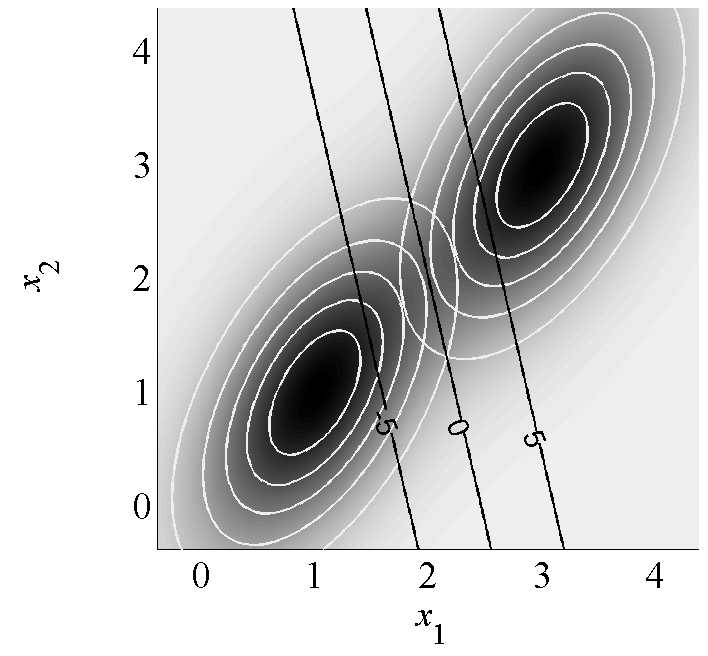
\includegraphics[width=6cm]{Figures/DecGauss2Deqv.pdf}
			\captionof{figure}{Decision boundaries of the LLRT and likelihoods for a Gaussian detection problem with 2D observations and identical covariance matrices.}
			\label{Dec:DecGauss2Deqv}
		\end{center}
	%\end{figure}
\end{example}

\begin{example}[Matched filter]
	In this example, we derive one of the most well-known detectors, the matched filter (MF). The MF is the LLRT to the detection of a known signal contaminated by zero-mean Gaussian noise. Concretely, under hypothesis $h=0$, the observations are given by noise only:
	\begin{equation*}
	x[n] = w[n], \quad n = 0, \ldots, N-1,
	\end{equation*}
	and under  hypothesis $h=1$, the observations are
	\begin{equation*}
	x[n] = s[n] + w[n], \quad n = 0, \ldots, N-1,
	\end{equation*}
	where $s[n]$ is a known signal and $w[n]$ is additive white Gaussian noise with zero mean and variance $\sigma^2$, i.e., $w[n] \sim \Normal(0,\sigma^2)$. To use the LLRT already derived in this section, we must first define the vector
	\begin{equation*}
	{\bf x} = \begin{pmatrix} x[0] & x[1] & \cdots & x[N-1] \end{pmatrix}^T = {\bf s} + {\bf w},
	\end{equation*}
	with ${\bf s} = \begin{pmatrix} s[0] & s[1] & \cdots & s[N-1] \end{pmatrix}^T $ and ${\bf w} = \begin{pmatrix} w[0] & w[1] & \cdots & w[N-1] \end{pmatrix}^T$, and obtain the distributions of ${\bf x}$ under both hypothesis. Under hypothesis $h=0$, the observation vector ${\bf x}$ collects samples of a Gaussian process, which makes it also Gaussian. Hence, only the mean and cross-covariance matrices are required:
	\begin{equation*}
	{\bf m}_0 = \mathbb{E}\{{\bf x}|0\} = \mathbb{E}\{{\bf w}\} = \begin{pmatrix} \mathbb{E}\{w[0]\}  & \mathbb{E}\{w[1]\} & \cdots & \mathbb{E}\{w[N-1]\} \end{pmatrix}^T = \mathbf{0},
	\end{equation*}
    and
	\begin{align*}
		{\bf V}_0 &= \mathbb{E}\left\{({\bf x} - {\bf m}_0) ({\bf x} - {\bf m}_0)^T|0\right\} = \mathbb{E}\left\{{\bf w} {\bf w}^T\right\} \\ &= \mathbb{E}\left\{\begin{pmatrix} w[0] & w[1] & \cdots & w[N-1] \end{pmatrix}^T \begin{pmatrix} w[0] & w[1] & \cdots & w[N-1] \end{pmatrix}\right\} \\
		&= \begin{pmatrix} \mathbb{E}\left\{w^2[0]\right\}  & \mathbb{E}\left\{w[0]w[1] \right\}& \cdots & \mathbb{E}\left\{w[0]w[N-1]\right\} \\ \mathbb{E}\left\{w[1] w[0]\right\} & \mathbb{E}\left\{w^2[1]\right\} & \cdots & \mathbb{E}\left\{w[1]w[N-1]\right\} \\ \vdots & \vdots & \ddots & \vdots   \\ \mathbb{E}\left\{w[N-1] w[0]\right\} & \mathbb{E}\left\{w[N-1] w[1]\right\} & \cdots & \mathbb{E}\left\{w^2[N-1] \right\} \end{pmatrix}.
 	\end{align*}
	The cross-covariance matrix ${\bf V}_0$ can be simplified taking into account that the noise is white, i.e., $\mathbb{E}\{w[n] w[n-m]\} = \sigma^2 \delta[m]$, which yields 
	\begin{equation*}
		{\bf V}_0 = \begin{pmatrix} \sigma^2  & 0 & \cdots & 0 \\ 0 & \sigma^2 & \cdots & 0 \\ \vdots & \vdots & \ddots & \vdots   \\ 0 & 0 & \cdots & \sigma^2 \end{pmatrix} = \sigma^2 \mathbf{I}.
\end{equation*}
Similarly, under hypothesis $h=1$, the observations are Gaussian with mean
\begin{equation*}
	{\bf m}_1 = \mathbb{E}\{{\bf x}|1\} = \mathbb{E}\{{\bf s} + {\bf w}\} = \mathbb{E}\{{\bf s}\} + \mathbb{E}\{{\bf w}\} = {\bf s},
\end{equation*}
since ${\bf s}$ is deterministic, and cross-covariance matrix
	\begin{equation*}
{\bf V}_1 = \mathbb{E}\left\{({\bf x} - {\bf m}_1) ({\bf x} - {\bf m}_1)^T|1\right\} = \mathbb{E}\left\{({\bf s} + {\bf w} - {\bf s}) ({\bf s} + {\bf w} - {\bf s})^T\right\} = \mathbb{E}\left\{{\bf w} {\bf w}^T\right\} = \sigma^2 \mathbf{I}.
\end{equation*}
Hence, the detection problem is that of Gaussian observations with identical covariance matrices, for which the LLRT is
\begin{equation*}
({\bf m}_1-{\bf m}_0)^T {\bf V}^{-1}{\bf x} = \frac{1}{\sigma^2} {\bf s}^T {\bf x} \dunodcero \tilde{\mu} \Rightarrow \underbrace{\sum_{n = 0}^{N-1} s[n]x[n]}_{MF} \ \dunodcero \sigma^2 \tilde{\mu}.
\end{equation*}
Alternatively, and the motivation for the term matched filter, is because the above detector can be rewritten as a filtering of the signal $x[n]$ with the filter $h[n] = s[N-1 - n]$, followed by sampling every $N$ samples. Finally, we also would like to point out that the matched filter is a filter that maximizes the signal-to-noise ratio.

\end{example}

\subsection{Zero means}

We consider now that ${\bf m}_0 = {\bf m}_1 = \mathbf{0}$, which yields
\begin{equation*}
{\bf x}^T \left({\bf V}_0^{-1}-{\bf V}_1^{-1}\right){\bf x} \dunodcero \mu.
\label{eq:logLRTGauss2m0}
\end{equation*}

\begin{example}
	Figure \ref{fig:DecGauss2Deqm} shows the ML decision boundary for 2D Gaussian observations with
		\begin{equation*}
{\bf m}_0 =  \left(\begin{array}{l}  0\\0   \end{array}\right), {\bf V}_0 = 
\left(\begin{array}{ll} 0.62 & -0.22 \\ -0.22 & 0.37 \end{array} \right),
\end{equation*}
and
\begin{equation*}
{\bf m}_1 = \left(\begin{array}{l}  0\\0  \end{array}\right), {\bf V}_1 = 
\left(\begin{array}{ll} 1 & 0 \\ 0 & 2 \end{array} \right).
\end{equation*}
	The region ${\cal X}_0$ is given by the interior of the ellipse. Moreover, since the variance of the observations in every direction is larger under hypothesis $h=1$, points further away from the origin should be assigned $d=1$.
	%\begin{figure}[htb]
		\begin{center}
			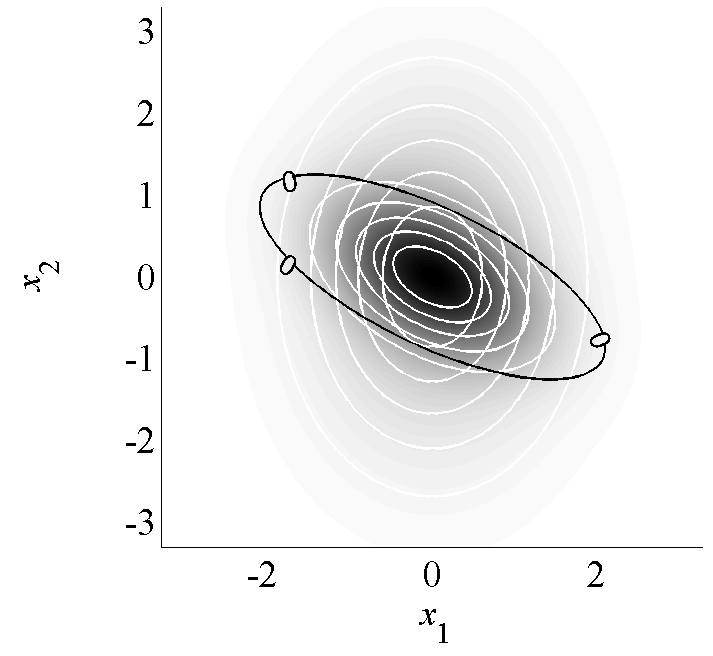
\includegraphics[width=6cm]{Figures/DecGauss2Deqm.pdf}
			\captionof{figure}{Elliptic decision boundary for a 2D Gaussian problem with zero means.}
			\label{fig:DecGauss2Deqm}
		\end{center}
	%\end{figure}
\end{example}

\begin{example}
	Figure \ref{fig:DecGauss2Deqm2} shows the ML decision boundary for 2D Gaussian observations with
	\begin{equation*}
	{\bf m}_0 =  \left(\begin{array}{l}  0\\0   \end{array}\right), {\bf V}_0 = 
	\left(\begin{array}{ll} 0.33 & 0.39 \\ 0.39 & 0.77  \end{array} \right)
	\end{equation*}
	and
	\begin{equation*}
	{\bf m}_1 = \left(\begin{array}{l}  0\\0  \end{array}\right), {\bf V}_1 = 
	\left(\begin{array}{ll} 0.39 &-0.19 \\ -0.19 & 0.16\end{array} \right).
	\end{equation*}
	In this example, the variance under hypothesis $h=1$ is larger only along dimension 1, whereas it is smaller along dimension 2. Hence, as a consequence, the boundary is a hyperbola.
	%\begin{figure}[htb]
		\begin{center}
			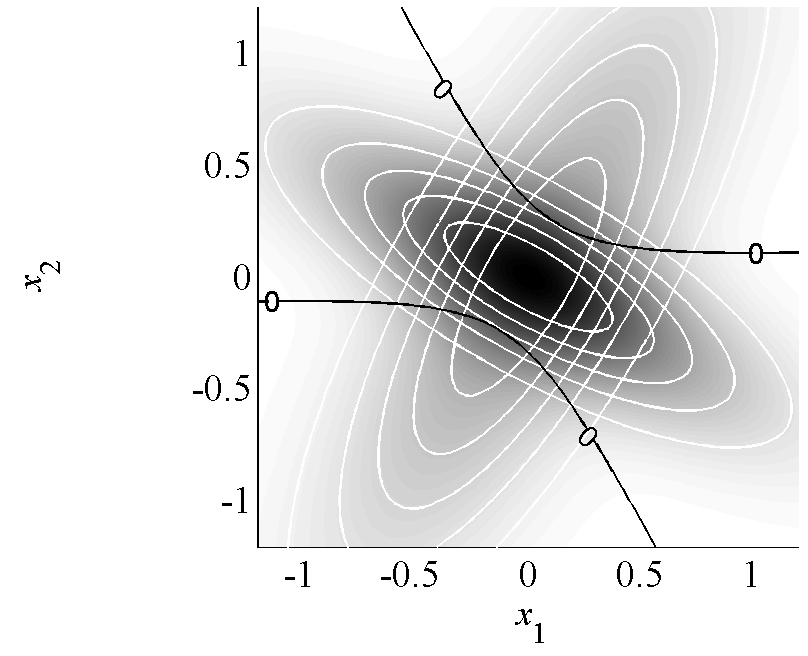
\includegraphics[width=6cm]{Figures/DecGauss2Deqm2.pdf}
			\captionof{figure}{Hyperbolic decision boundary for a 2D Gaussian problem with zero means.}
			\label{fig:DecGauss2Deqm2}
		\end{center}
	%\end{figure}
\end{example}

%\subsection{Summary of most relevant expressions}
%\subsubsection{General case}
%\begin{itemize}
%    \item Probability of error
%    $$P_e = P(D\neq H) = 1 - P(D=H)$$
%    \item Probability of error given ${\bf x}$
%    $$P(d\neq H|{\bf x}) = 1 - P(d = H|{\bf x}) = 1 - P_{H|{\bf X}}(d|{\bf x})$$
%    \item Mean cost
%    $$\mathbb{E}\left\{ c_{DH}\right\} = \sum_{h=0}^{M-1} \sum_{d=0}^{M-1} c_{dh} P(D=d, H=h)$$
%    \item Mean cost given $\bf x$
%    $$\mathbb{E}\left\{ c_{dH}\right|{\bf x}\} = \sum_{h=0}^{M-1} c_{dh} P_{H|X}(h|{\bf x})$$
%    \item ML classifier
%    $$d_{ML} = \arg\max_h p_{{\bf X}|H}({\bf x}|h)$$
%    \item MAP classifier
%    $$d_{MAP} = \arg\max_h P_{H|{\bf X}}(h|{\bf x})$$
%    \item Minimum mean cost classifier
%    $$d^\star = \arg\min_{d} \sum_{h=0}^{M-1} c_{dh} P_{H|X}(h|{\bf x})$$
%\end{itemize}
%
%\subsubsection{Binary case}
%\begin{itemize}
%    \item Probability of error
%    $$P_e = P_\text{M} P_H(1) + P_\text{FA} P_H(0)$$
%    \item Probability of False Alarm, Missing and Detection
%    \begin{align}
%        P_\text{FA} & = P(D=1|H=0) = \int_{{\cal X}_1} p_{\bf X|H}({\bf x}|0) d{\bf x} \nonumber \\
%        P_\text{M} & = P(D=0|H=1) = \int_{{\cal X}_0} p_{\bf X|H}({\bf x}|1) d{\bf x} \nonumber \\
%        P_\text{D} & = P(D=1|H=1) = 1 - P_\text{M} \nonumber
%    \end{align}
%    \item Likelihood ratio test:
%    $$\displaystyle\frac{p_{{\bf X}|H}({\bf x}|1)}{p_{{\bf X}|H}({\bf x}|0)} \dunodcero \eta$$
%    Some particular cases are:
%    \begin{itemize}
%        \item ML classifier: $\eta_{ML} = 1$
%        \item MAP classifier: $\eta_{MAP} = \displaystyle\frac{P_H(0)}{P_H(1)}$
%        \item Minimum mean cost classifier: $\eta^\star = \displaystyle\frac{c_{10}-c_{00}}{c_{01}-c_{11}} \displaystyle\frac{P_H(0)}{P_H(1)}$
%    \end{itemize}
%
%\end{itemize}



%%%%%%%%%%%%%%%%%%%
\section{Problems}
%%%%%%%%%%%%%%%%%%%

%
%%%%%%%%%%%%
\begin{prob}
\label{MAPmulticlas}

Consider the decision problem with three hypotheses given by the observation ${\bf x}=(x_1,x_2) \in [0,1]^2$ and likelihoods:
\begin{equation}
p_{{\bf X}|H}({\bf x}|0) = 2(1-x_1)
\end{equation}
\begin{equation}
p_{{\bf X}|H}({\bf x}|1) = 2 x_1
\end{equation}
\begin{equation}
p_{{\bf X}|H}({\bf x}|2) = 2 x_2
\end{equation}

\begin{enumerate}[a)]
\item Determine the ML (Maximum Likelihood) classifier
\item Represent the decision regions.
\end{enumerate}
\end{prob}
%%%%%%%%%%


%%%%%%%%%%%%
\begin{prob}
\label{PFAPMPE}

Consider the decision problem given by the observation $x \in [0,1]$, likelihoods:
\begin{equation}
p_{X|H}(x|0) = 2(1-x)
\end{equation}
\begin{equation}
p_{X|H}(x|1) = 1
\end{equation}
and prior probability $P_H(1)=1/4$.

\begin{enumerate}[a)]
\item Determine the ML classifier.
\item Determine the MAP (Maximum A Posteriori) classifier.
\item Given that $c_{01}=2$, $c_{10}=1$, $c_{11}=c_{00}=0$, determine the decision-maker of minimum risk.
\item Consider a threshold detector over $x$ in the form:
\begin{equation}
x \dunodcero \eta
\end{equation}
Calculate the probabilities of false alarm, miss and error, as a function of $\eta$.
\item Apply the result to the previous three decision-makers. Verify that the MAP classifier obtains the minimum probability of error.
\item Determine the risk for the previous three decision-makers, using the cost parameters from part (c), and verify that the decision-maker obtained in said part achieves the lowest risk.
\end{enumerate}

\end{prob}
%%%%%%%%%%



%%%%%%%%%%%%
\begin{prob}
\label{ProbDecMLbin}

Consider a one-dimensional binary decision problem with equiprobable hypotheses, defined by the likelihoods:
\begin{align}
p_{X|H}(x|0) = & \frac{1}{6},    \ \ \ |x| \leq 3,  \nonumber \\
p_{X|H}(x|1) = & \frac{3}{2} x^2,\ \ \ |x| \leq 1   \nonumber                         
\end{align}

\begin{enumerate}[a)]
\item Determine the ML (Maximum Likelihood) classifier.
\item Determine the values of $\pfa$ (false alarm probability), $\pmis$ (miss probability), and $P_{\text{e}}$ (error probability) for the above classifier.
\end{enumerate}

\end{prob}
%%%%%%%%%%


%%%%%%%%%%%%
\begin{prob}
\label{ROCexp}

Consider the decision problem defined by the observation $x \ge 0$ and likelihoods:
\begin{equation}
p_{X|H}(x|0) = \exp(-x);
\end{equation}
\begin{equation}
p_{X|H}(x|1) = 2 \exp(-2x);
\end{equation}

\begin{enumerate}[a)]
\item Determine the LRT (Likelihood Ratio Test) decision rule.
\item Determine the ROC (Receiver Operating Characteristic).
\end{enumerate}

\end{prob}
%%%%%%%%%%


%%%%%%%%%%%%
\begin{prob}
\label{ProbDecLRTUnifPoison}

Consider a binary decision problem where the likelihood for hypothesis $H = 0$ is uniform over the interval $0 < x < 1$, while $p_{X|H}(x|1) = 2 x$, $0 < x < 1$.

\begin{enumerate}[a)]
\item Obtain the general expression for a Likelihood Ratio Test with parameter $\eta$. Graphically represent both likelihoods on the same axes, indicating the decision regions for the ML case.
\item Obtain the analytic expression of the ROC curve for the LRT. Plot this curve indicating the operating points for the ML classifier and the Neyman-Pearson detector with parameter $\alpha = 0.1$ (i.e., $\pfa \leq \alpha = 0.1$).
\end{enumerate}

\end{prob}
%%%%%%%%%%%



%%%%%%%%%%%%
\begin{prob}
\label{RealProb}

Company E manufactures 10,000 units of a product daily. It has been estimated that:
\begin{itemize}
\item The sale of a unit in good condition nets a profit of 3 Euros.
\item Placing a defective unit on the market causes (on average) a loss of 81 Euros.
\item The withdrawal of a unit (whether defective or not) results in a loss of 1 Euro.
\end{itemize}

An automatic inspection system is available that obtains, for each unit, an observation $x_1$. Defining $H=0$ as the hypothesis "the unit is not defective" and $H=1$ as "the unit is defective",
\begin{equation}
p_{X_1|H}(x_1|0) = \exp(-x_1)u(x_1)
\end{equation}
\begin{equation}
p_{X_1|H}(x_1|1) = \lambda_1 \exp(-\lambda_1 x_1)u(x_1)
\end{equation}
where $\lambda_1=1/2$. Additionally, the assembly line produces, on average, one defective unit for every 100 non-defective ones.
    
The aim is to incorporate an automatic mechanism for withdrawing defective units based on the observation of $x_1$.

\begin{enumerate}[a)]
\item Design the detector that provides Company E with the highest expected profit.
\item Determine the maximum expected daily profit that can be achieved.
\item A company offers Company E an innovative inspection device that provides, for each product, in addition to $x_1$, a new observation $x_2$, statistically independent from $x_1$, such that
\begin{equation}
p_{X_2|H}(x_2|0) = \exp(-x_2)u(x_2)
\end{equation}
\begin{equation}
p_{X_2|H}(x_2|1) = \lambda_2 \exp(-\lambda_2 x_2)u(x_2)
\end{equation}
where $\lambda_2 = 1/4$. The cost of this machine is 6000 Euros. Determine an expression for the {average time} it would take Company E to amortize this machine.
\end{enumerate}
\end{prob}
%%%%%%%%%%
%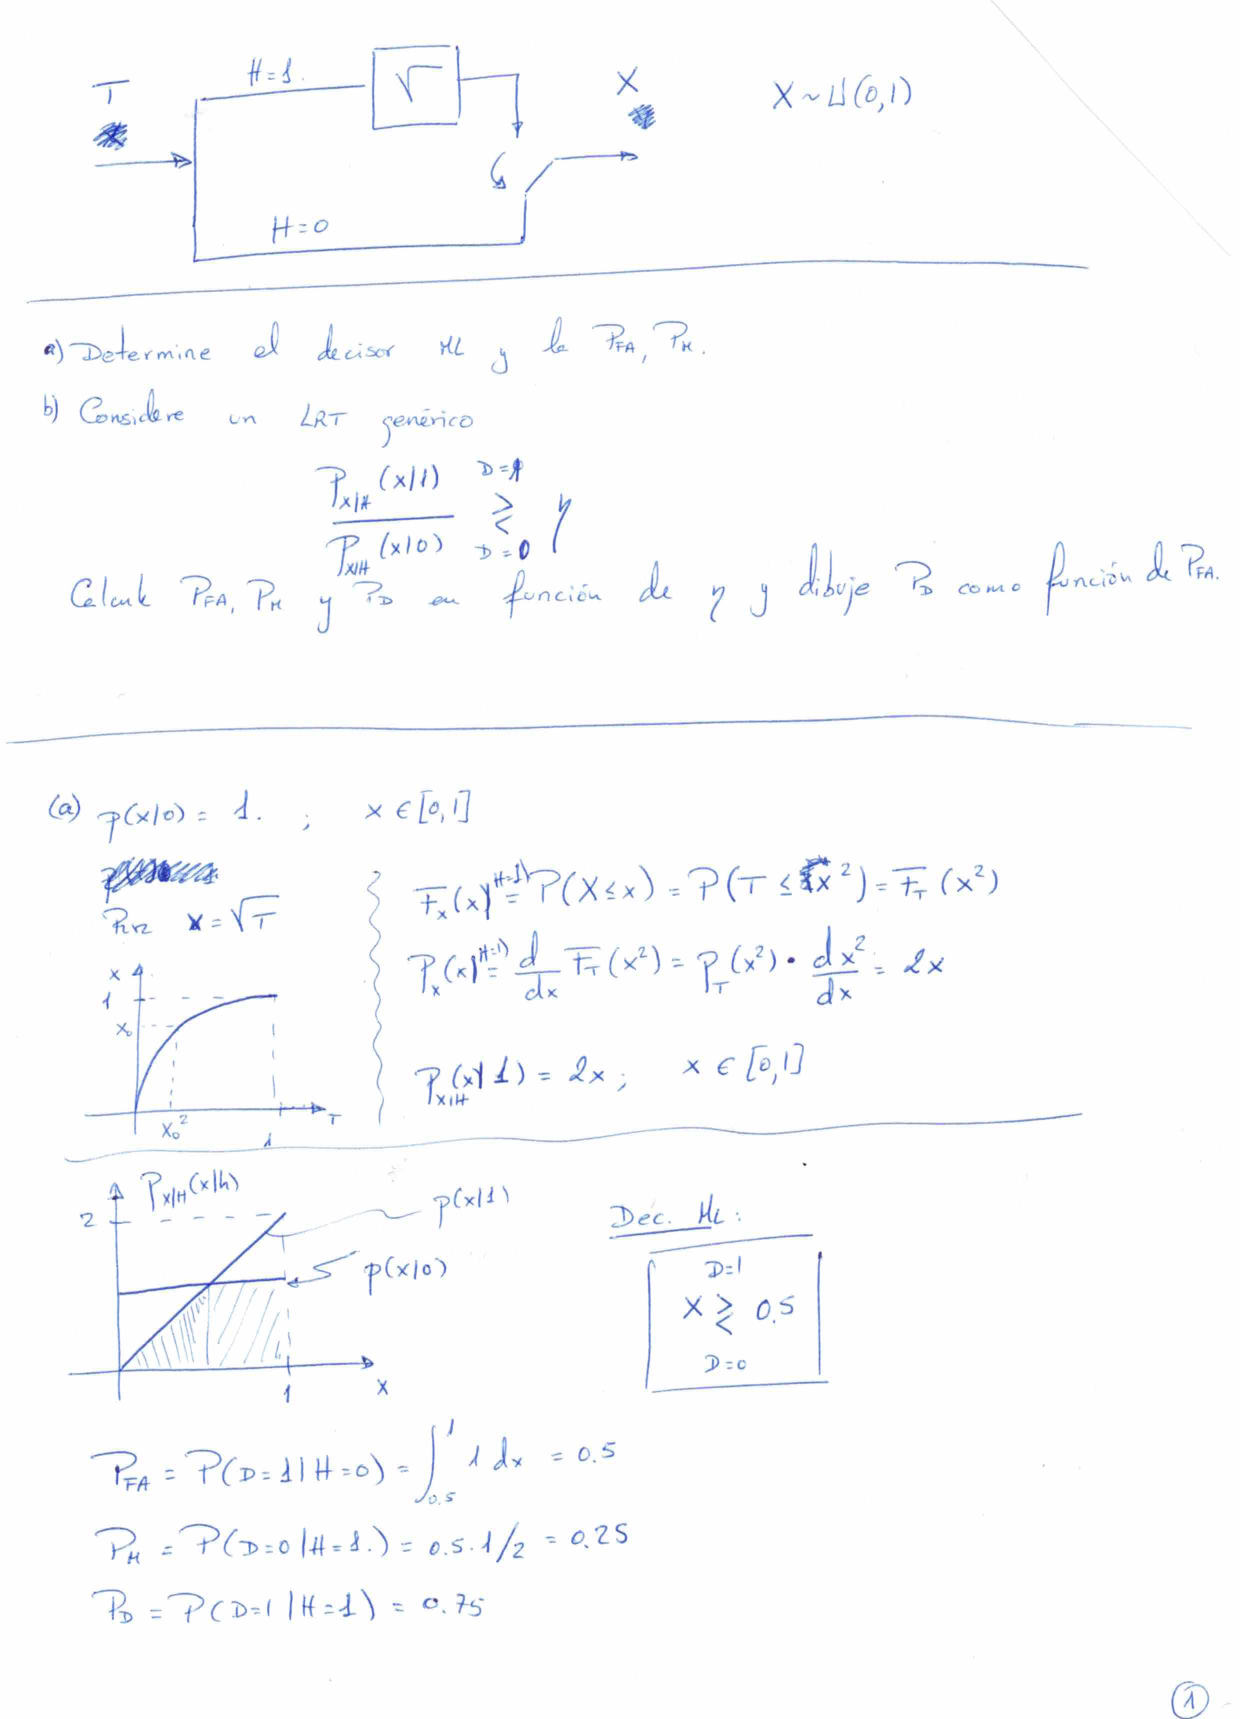
\includepdf[pages=-]{Contents/decision/LRT_Labo_Clas_problem}

\backmatter
\printindex
%%%%%%%%%%%%%%%%%%%%%%%%%%%%%%%%%%%%%%%%%%%%%%%%%%%%%%%%%%%%%%%%%%%%%%

\end{document}

\end{thebibliography}

\end{document}



























